%%%%%%%%%%%%%%%%%%%%%%%%%%%%%%%%%%%%%%%%%%%%%%%%%%%%%%%%%%%%%%%%%%%%%%
% Template for a UBC-compliant dissertation
% At the minimum, you will need to change the information found
% after the "Document meta-data"
%
%!TEX TS-program = pdflatex
%!TEX encoding = UTF-8 Unicode

%% The ubcdiss class provides several options:
%%   fogscopy
%%       set parameters to exactly how FoGS specifies
%%         * single-sided
%%         * page-numbering starts from title page
%%         * the lists of figures and tables have each entry prefixed
%%           with 'Figure' or 'Table'
%%       This can be tested by `\iffogscopy ... \else ... \fi'
%%   10pt, 11pt, 12pt
%%       set default font size
%%   oneside, twoside
%%       whether to format for single-sided or double-sided printing
%%   balanced
%%       when double-sided, ensure page content is centred
%%       rather than slightly offset (the default)
%%   singlespacing, onehalfspacing, doublespacing
%%       set default inter-line text spacing; the ubcdiss class
%%       provides \textspacing to revert to this configured spacing
%%   draft
%%       disable more intensive processing, such as including
%%       graphics, etc.
%%

% For submission to FoGS
\documentclass[fogscopy,onehalfspacing,11pt]{ubcdiss}

% For your own copies (looks nicer)
% \documentclass[balanced,twoside,11pt]{ubcdiss}

%%%%%%%%%%%%%%%%%%%%%%%%%%%%%%%%%%%%%%%%%%%%%%%%%%%%%%%%%%%%%%%%%%%%%%
%%%%%%%%%%%%%%%%%%%%%%%%%%%%%%%%%%%%%%%%%%%%%%%%%%%%%%%%%%%%%%%%%%%%%%
%%
%% FONTS:
%% 
%% The defaults below configures Times Roman for the serif font,
%% Helvetica for the sans serif font, and Courier for the
%% typewriter-style font.  Configuring fonts can be time
%% consuming; we recommend skipping to END FONTS!
%% 
%% If you're feeling brave, have lots of time, and wish to use one
%% your platform's native fonts, see the commented out bits below for
%% XeTeX/XeLaTeX.  This is not for the faint at heart. 
%% (And shouldn't you be writing? :-)
%%

%% NFSS font specification (New Font Selection Scheme)
\usepackage{times,mathptmx,courier}
\usepackage[scaled=.92]{helvet}

%% Math or theory people may want to include the handy AMS macros
\usepackage{amssymb}
\usepackage{amsmath}
\usepackage{amsfonts}
\usepackage{bm} %bold math

%% The pifont package provides access to the elements in the dingbat font.   
%% Use \ding{##} for a particular dingbat (see p7 of psnfss2e.pdf)
%%   Useful:
%%     51,52 different forms of a checkmark
%%     54,55,56 different forms of a cross (saltyre)
%%     172-181 are 1-10 in open circle (serif)
%%     182-191 are 1-10 black circle (serif)
%%     192-201 are 1-10 in open circle (sans serif)
%%     202-211 are 1-10 in black circle (sans serif)
%% \begin{dinglist}{##}\item... or dingautolist (which auto-increments)
%% to create a bullet list with the provided character.
\usepackage{pifont}

%%%%%%%%%%%%%%%%%%%%%%%%%%%%%%%%%%%%%%%%%%%%%%%%%%%%%%%%%%%%%%%%%%%%%%
%% Configure fonts for XeTeX / XeLaTeX using the fontspec package.
%% Be sure to check out the fontspec documentation.
%\usepackage{fontspec,xltxtra,xunicode}	% required
%\defaultfontfeatures{Mapping=tex-text}	% recommended
%% Minion Pro and Myriad Pro are shipped with some versions of
%% Adobe Reader.  Adobe representatives have commented that these
%% fonts can be used outside of Adobe Reader.
%\setromanfont[Numbers=OldStyle]{Minion Pro}
%\setsansfont[Numbers=OldStyle,Scale=MatchLowercase]{Myriad Pro}
%\setmonofont[Scale=MatchLowercase]{Andale Mono}

%% Other alternatives:
%\setromanfont[Mapping=tex-text]{Adobe Caslon}
%\setsansfont[Scale=MatchLowercase]{Gill Sans}
%\setsansfont[Scale=MatchLowercase,Mapping=tex-text]{Futura}
%\setmonofont[Scale=MatchLowercase]{Andale Mono}
%\newfontfamily{\SYM}[Scale=0.9]{Zapf Dingbats}
%% END FONTS
%%%%%%%%%%%%%%%%%%%%%%%%%%%%%%%%%%%%%%%%%%%%%%%%%%%%%%%%%%%%%%%%%%%%%%
%%%%%%%%%%%%%%%%%%%%%%%%%%%%%%%%%%%%%%%%%%%%%%%%%%%%%%%%%%%%%%%%%%%%%%



%%%%%%%%%%%%%%%%%%%%%%%%%%%%%%%%%%%%%%%%%%%%%%%%%%%%%%%%%%%%%%%%%%%%%%
%%%%%%%%%%%%%%%%%%%%%%%%%%%%%%%%%%%%%%%%%%%%%%%%%%%%%%%%%%%%%%%%%%%%%%
%%
%% Recommended packages
%%
\usepackage{checkend}	% better error messages on left-open environments
\usepackage{graphicx}	% for incorporating external images

%% booktabs: provides some special commands for typesetting tables as used
%% in excellent journals.  Ignore the examples in the Lamport book!
\usepackage{booktabs}

%% listings: useful support for including source code listings, with
%% optional special keyword formatting.  The \lstset{} causes
%% the text to be typeset in a smaller sans serif font, with
%% proportional spacing.
\usepackage{listings}
\lstset{basicstyle=\sffamily\scriptsize,showstringspaces=false,fontadjust}

%% The acronym package provides support for defining acronyms, providing
%% their expansion when first used, and building glossaries.  See the
%% example in glossary.tex and the example usage throughout the example
%% document.
%% NOTE: to use \MakeTextLowercase in the \acsfont command below,
%%   we *must* use the `nohyperlinks' option -- it causes errors with
%%   hyperref otherwise.  See Section 5.2 in the ``LaTeX 2e for Class
%%   and Package Writers Guide'' (clsguide.pdf) for details.
\usepackage[printonlyused,nohyperlinks]{acronym}
%% The ubcdiss.cls loads the `textcase' package which provides commands
%% for upper-casing and lower-casing text.  The following causes
%% the acronym package to typeset acronyms in small-caps
%% as recommended by Bringhurst.
\renewcommand{\acsfont}[1]{{\scshape \MakeTextLowercase{#1}}}

%% color: add support for expressing colour models.  Grey can be used
%% to great effect to emphasize other parts of a graphic or text.
%% For an excellent set of examples, see Tufte's "Visual Display of
%% Quantitative Information" or "Envisioning Information".
\usepackage{color}
\definecolor{greytext}{gray}{0.5}

%% comment: provides a new {comment} environment: all text inside the
%% environment is ignored.
%%   \begin{comment} ignored text ... \end{comment}
\usepackage{comment}

%% The natbib package provides more sophisticated citing commands
%% such as \citeauthor{} to provide the author names of a work,
%% \citet{} to produce an author-and-reference citation,
%% \citep{} to produce a parenthetical citation.
%% We use \citeeg{} to provide examples
\usepackage[numbers,sort&compress]{natbib}
\newcommand{\citeeg}[1]{\citep[e.g.,][]{#1}}

%drawing circle around the number
\usepackage{tikz}
\usepackage{pifont}
%\ding{192} for 1

%% The titlesec package provides commands to vary how chapter and
%% section titles are typeset.  The following uses more compact
%% spacings above and below the title.  The titleformat that follow
%% ensure chapter/section titles are set in singlespace.
\usepackage[compact]{titlesec}
\titleformat*{\section}{\singlespacing\raggedright\bfseries\Large}
\titleformat*{\subsection}{\singlespacing\raggedright\bfseries\large}
\titleformat*{\subsubsection}{\singlespacing\raggedright\bfseries}
\titleformat*{\paragraph}{\singlespacing\raggedright\itshape}

%% The caption package provides support for varying how table and
%% figure captions are typeset.
\usepackage[format=hang,indention=-1cm,labelfont={bf},margin=1em]{caption}

%% url: for typesetting URLs and smart(er) hyphenation.
%% \url{http://...} 
\usepackage{url}
\urlstyle{sf}	% typeset urls in sans-serif



%%%%%%%%%%%%%%%%%%%%%%%%%%%%%%%%%%%%%%%%%%%%%%%%%%%%%%%%%%%%%%%%%%%%%%
%%%%%%%%%%%%%%%%%%%%%%%%%%%%%%%%%%%%%%%%%%%%%%%%%%%%%%%%%%%%%%%%%%%%%%
%%
%% Possibly useful packages: you may need to explicitly install
%% these from CTAN if they aren't part of your distribution;
%% teTeX seems to ship with a smaller base than MikTeX and MacTeX.
%%
%\usepackage{pdfpages}	% insert pages from other PDF files
%\usepackage{longtable}	% provide tables spanning multiple pages
%\usepackage{chngpage}	% support changing the page widths on demand
%\usepackage{tabularx}	% an enhanced tabular environment

%% enumitem: support pausing and resuming enumerate environments.
%\usepackage{enumitem}

%% rotating: provides two environments, sidewaystable and sidewaysfigure,
%% for typesetting tables and figures in landscape mode.  
%\usepackage{rotating}

%% subfig: provides for including subfigures within a figure,
%% and includes being able to separately reference the subfigures.
%\usepackage{subfig}

%% ragged2e: provides several new new commands \Centering, \RaggedLeft,
%% \RaggedRight and \justifying and new environments Center, FlushLeft,
%% FlushRight and justify, which set ragged text and are easily
%% configurable to allow hyphenation.
%\usepackage{ragged2e}

%% The ulem package provides a \sout{} for striking out text and
%% \xout for crossing out text.  The normalem and normalbf are
%% necessary as the package messes with the emphasis and bold fonts
%% otherwise.
%\usepackage[normalem,normalbf]{ulem}    % for \sout

%%%%%%%%%%%%%%%%%%%%%%%%%%%%%%%%%%%%%%%%%%%%%%%%%%%%%%%%%%%%%%%%%%%%%%
%% HYPERREF:
%% The hyperref package provides for embedding hyperlinks into your
%% document.  By default the table of contents, references, citations,
%% and footnotes are hyperlinked.
%%
%% Hyperref provides a very handy command for doing cross-references:
%% \autoref{}.  This is similar to \ref{} and \pageref{} except that
%% it automagically puts in the *type* of reference.  For example,
%% referencing a figure's label will put the text `Figure 3.4'.
%% And the text will be hyperlinked to the appropriate place in the
%% document.
%%
%% Generally hyperref should appear after most other packages

%% The following puts hyperlinks in very faint grey boxes.
%% The `pagebackref' causes the references in the bibliography to have
%% back-references to the citing page; `backref' puts the citing section
%% number.  See further below for other examples of using hyperref.
%% 2009/12/09: now use `linktocpage' (Jacek Kisynski): FoGS now prefers
%%   that the ToC, LoF, LoT place the hyperlink on the page number,
%%   rather than the entry text.
\usepackage[bookmarks,bookmarksnumbered,%
    citebordercolor={0.8 0.8 0.8},filebordercolor={0.8 0.8 0.8},%
    linkbordercolor={0.8 0.8 0.8},pagebordercolor={0.8 0.8 0.8},%
    urlbordercolor={0.8 0.8 0.8},%
    pagebackref,linktocpage%
    ]{hyperref}
%% The following change how the the back-references text is typeset in a
%% bibliography when `backref' or `pagebackref' are used
\renewcommand\backrefpagesname{\(\rightarrow\) pages}
\renewcommand\backref{\textcolor{greytext} \backrefpagesname\ }

% the following user-defined commands are used by my two papers
\newcommand{\bra}[1]{\langle #1 |}
\newcommand{\ket}[1]{| #1 \rangle}
\newcommand{\braket}[2]{\langle #1 | #2 \rangle}
\newcommand{\matelement}[3]{\langle #1 | #2 | #3 \rangle}
\newcommand{\beq}{\begin{equation}}
\newcommand{\eeq}{\end{equation}}
\newcommand{\crea}[3]{\hat #1^{\dagger}_{#2,#3}}
\newcommand{\anni}[3]{\hat #1_{#2,#3}}

\newcommand{\creation}[2]{\hat #1^{\dagger}_{#2}}
\newcommand{\annihilation}[2]{\hat #1_{#2}}

\newcommand{\pd}[1]{\hat{P}^{\dagger}_{#1}}
\newcommand{\p}[1]{\hat{P}_{#1}}

\newcommand{\threejm}[6]{ \left(\begin{array}{ccc} #1 & #3 & #5\\
                                              #2 & #4 & #6
                                \end{array}
                          \right)}

\newcommand{\oneline}[1] {
\begin{equation}
#1
\end{equation}
}

\newcommand{\multiline}[1] {
\begin{eqnarray}
#1
\end{eqnarray}
}

% a short cut to make figure
\newcommand{\addfigure}[1]{
\begin{figure}[htbp]
\centering
#1
\end{figure}
}
                          
\def\vec#1{\mathbf{#1}}
\def\k{\mathbf{k}}
\def\q{\mathbf{q}}
\def\ri{\mathbf{r}_i}
\def\rj{\mathbf{r}_j}
\def\xi{\mathbf{x}_i}
\def\xj{\mathbf{x}_j}
\def\Ri{\mathbf{R}_i}
\def\Rj{\mathbf{R}_j}
\def\dA{\mathbf{d}_A}
\def\dB{\mathbf{d}_B}
\def\R{\mathbf{\hat{R}}}


\def\vp{\Phi}
\def\D{\Delta}

%%%%%%%%%%%%% customize autoref package %%%%%%%%%%%%%%%%%%%%%%%%%


%\let\orgautoref\autoref
%\providecommand{\Autoref}[1]
%        {%\def\equationautorefname{Equation}%
%         \def\figureautorefname{Figure}%
%         \def\subfigureautorefname{Figure}%
%         \def\Itemautorefname{Item}%
%         \def\tableautorefname{Table}%
%         \def\sectionautorefname{Section}%
%         \def\subsectionautorefname{Section}%
%         \def\subsubsectionautorefname{Section}%
%         \def\chapterautorefname{Section}%
%         \def\partautorefname{Part}%
%	\def\equationautorefname~#1{Equation~(#1)}%
%  	\autoref{#1}%
%         \orgautoref}

  \def\chapterautorefname~#1\null{chapter~(#1)\null}%
  \def\sectionautorefname~#1\null{section~(#1)\null}%
  \def\subsectionautorefname~#1\null{section~(#1)\null}%
  \def\figureautorefname~#1\null{figure~(#1)\null}%
  \def\tableautorefname~#1\null{table~(#1)\null}%
  \def\equationautorefname~#1\null{equation~(#1)\null}%

\newcommand{\Autoref}[1]{%
  \begingroup%
  \def\chapterautorefname~##1\null{Chapter~(##1)\null}%
  \def\sectionautorefname~##1\null{Section~(##1)\null}%
  \def\subsectionautorefname~##1\null{Section~(##1)\null}%
  \def\figureautorefname~##1\null{Figure~(##1)\null}%
  \def\tableautorefname~##1\null{Table~(##1)\null}%
  \def\equationautorefname~##1\null{Equation~(##1)\null}%
  \autoref{#1}%
  \endgroup%
}

%\renewcommand{\autoref}
%        {%\def\equationautorefname{equation}%
%         \def\figureautorefname{figure}%
%         \def\subfigureautorefname{figure}%
%         \def\Itemautorefname{item}%
%         \def\tableautorefname{table}%
%         \def\sectionautorefname{section}%
%         \def\subsectionautorefname{section}%
%         \def\subsubsectionautorefname{section}%
%         \def\chapterautorefname{section}%
%         \def\partautorefname{part}%
%         \orgautoref}

%\renewcommand{\autoref}[1]{ %
%  \def\chapterautorefname~#1\null{chapter~(#1)\null}%
%  \def\sectionautorefname~#1\null{section~(#1)\null}%
%  \def\subsectionautorefname~#1\null{section~(#1)\null}%
%  \def\figureautorefname~#1\null{figure~(#1)\null}%
%  \def\tableautorefname~#1\null{table~(#1)\null}%
%  \def\equationautorefname~#1\null{equation~(#1)\null}%
%}

%\def\equationautorefname~#1\null{%
%  equation~(#1)\null
%}

%%%%%%%%%%%%%%%%%%%%%%%%%%%%%%%%%%%%%%%%%%%%%%%%
\newcommand*\circled[1]{\tikz[baseline=(char.base)]{
  \node[shape=circle,draw,inner sep=1.0pt] (char) {#1};}}

%%%%%%%%%%%%%%%%%%%%%%%%%%%%%%%%%%%%%%%%%%%%%

%%%%%% customize the position of figures%%%%%%%%%%%%%%%%%%%
\renewcommand{\textfraction}{0.15}
\renewcommand{\topfraction}{0.85}
\renewcommand{\bottomfraction}{0.65}
\renewcommand{\floatpagefraction}{0.60}


%% The following uses most defaults, which causes hyperlinks to be
%% surrounded by colourful boxes; the colours are only visible in
%% PDFs and don't show up when printed:
%\usepackage[bookmarks,bookmarksnumbered]{hyperref}

%% The following disables the colourful boxes around hyperlinks.
%\usepackage[bookmarks,bookmarksnumbered,pdfborder={0 0 0}]{hyperref}

%% The following disables all hyperlinking, but still enabled use of
%% \autoref{}
%\usepackage[draft]{hyperref}

%% The following commands causes chapter and section references to
%% uppercase the part name.
\renewcommand{\chapterautorefname}{Chapter}
\renewcommand{\sectionautorefname}{Section}
\renewcommand{\subsectionautorefname}{Section}
\renewcommand{\subsubsectionautorefname}{Section}

%% If you have long page numbers (e.g., roman numbers in the 
%% preliminary pages for page 28 = xxviii), you might need to
%% uncomment the following and tweak the \@pnumwidth length
%% (default: 1.55em).  See the tocloft documentation at
%% http://www.ctan.org/tex-archive/macros/latex/contrib/tocloft/
% \makeatletter
% \renewcommand{\@pnumwidth}{3em}
% \makeatother

%%%%%%%%%%%%%%%%%%%%%%%%%%%%%%%%%%%%%%%%%%%%%%%%%%%%%%%%%%%%%%%%%%%%%%
%%%%%%%%%%%%%%%%%%%%%%%%%%%%%%%%%%%%%%%%%%%%%%%%%%%%%%%%%%%%%%%%%%%%%%
%%
%% Some special settings that controls how text is typeset
%%
% \raggedbottom		% pages don't have to line up nicely on the last line
% \sloppy		% be a bit more relaxed in inter-word spacing
% \clubpenalty=10000	% try harder to avoid orphans
% \widowpenalty=10000	% try harder to avoid widows
% \tolerance=1000

%% And include some of our own useful macros
% This file provides examples of some useful macros for typesetting
% dissertations.  None of the macros defined here are necessary beyond
% for the template documentation, so feel free to change, remove, and add
% your own definitions.
%
% We recommend that you define macros to separate the semantics
% of the things you write from how they are presented.  For example,
% you'll see definitions below for a macro \file{}: by using
% \file{} consistently in the text, we can change how filenames
% are typeset simply by changing the definition of \file{} in
% this file.
% 
%% The following is a directive for TeXShop to indicate the main file
%%!TEX root = diss.tex

\newcommand{\NA}{\textsc{n/a}}	% for "not applicable"
\newcommand{\eg}{e.g.,\ }	% proper form of examples (\eg a, b, c)
\newcommand{\ie}{i.e.,\ }	% proper form for that is (\ie a, b, c)
\newcommand{\etal}{\emph{et al}}

% Some useful macros for typesetting terms.
\newcommand{\file}[1]{\texttt{#1}}
\newcommand{\class}[1]{\texttt{#1}}
\newcommand{\latexpackage}[1]{\href{http://www.ctan.org/macros/latex/contrib/#1}{\texttt{#1}}}
\newcommand{\latexmiscpackage}[1]{\href{http://www.ctan.org/macros/latex/contrib/misc/#1.sty}{\texttt{#1}}}
\newcommand{\env}[1]{\texttt{#1}}
\newcommand{\BibTeX}{Bib\TeX}

% Define a command \doi{} to typeset a digital object identifier (DOI).
% Note: if the following definition raise an error, then you likely
% have an ancient version of url.sty.  Either find a more recent version
% (3.1 or later work fine) and simply copy it into this directory,  or
% comment out the following two lines and uncomment the third.
\DeclareUrlCommand\DOI{}
\newcommand{\doi}[1]{\href{http://dx.doi.org/#1}{\DOI{doi:#1}}}
%\newcommand{\doi}[1]{\href{http://dx.doi.org/#1}{doi:#1}}

% Useful macro to reference an online document with a hyperlink
% as well with the URL explicitly listed in a footnote
% #1: the URL
% #2: the anchoring text
\newcommand{\webref}[2]{\href{#1}{#2}\footnote{\url{#1}}}

% epigraph is a nice environment for typesetting quotations
\makeatletter
\newenvironment{epigraph}{%
	\begin{flushright}
	\begin{minipage}{\columnwidth-0.75in}
	\begin{flushright}
	\@ifundefined{singlespacing}{}{\singlespacing}%
    }{
	\end{flushright}
	\end{minipage}
	\end{flushright}}
\makeatother

% \FIXME{} is a useful macro for noting things needing to be changed.
% The following definition will also output a warning to the console
\newcommand{\FIXME}[1]{\typeout{**FIXME** #1}\textbf{[FIXME: #1]}}

% END


%%%%%%%%%%%%%%%%%%%%%%%%%%%%%%%%%%%%%%%%%%%%%%%%%%%%%%%%%%%%%%%%%%%%%%
%%%%%%%%%%%%%%%%%%%%%%%%%%%%%%%%%%%%%%%%%%%%%%%%%%%%%%%%%%%%%%%%%%%%%%
%%
%% Document meta-data: be sure to also change the \hypersetup information
%%

\title{Quantum control of dynamics of particles in a periodic lattice potential}
%\subtitle{If you want a subtitle}

\author{Ping Xiang}
\previousdegree{Bachelor of Science, Nankai University, 2007}
%\previousdegree{M. Silly Walks, Another University, 1994}

% What is this dissertation for?
\degreetitle{Doctor of Philosophy}

\institution{The University Of British Columbia}
\campus{Vancouver}

\faculty{The Faculty of Graduate Studies}
\department{Chemistry}
\submissionmonth{June}
\submissionyear{2014}

%% hyperref package provides support for embedding meta-data in .PDF
%% files
\hypersetup{
  pdftitle={Change this title!  (DRAFT: \today)},
  pdfauthor={Ping Xiang},
  pdfkeywords={thesis}
}

%%%%%%%%%%%%%%%%%%%%%%%%%%%%%%%%%%%%%%%%%%%%%%%%%%%%%%%%%%%%%%%%%%%%%%
%%%%%%%%%%%%%%%%%%%%%%%%%%%%%%%%%%%%%%%%%%%%%%%%%%%%%%%%%%%%%%%%%%%%%%
%% 
%% The document content
%%

%% LaTeX's \includeonly commands causes any uses of \include{} to only
%% include files that are in the list.  This is helpful to produce
%% subsets of your thesis (e.g., for committee members who want to see
%% the dissertation chapter by chapter).  It also saves time by 
%% avoiding reprocessing the entire file.
%\includeonly{intro,conclusions}
%\includeonly{discussion}

\begin{document}

%%%%%%%%%%%%%%%%%%%%%%%%%%%%%%%%%%%%%%%%%%%%%%%%%%
%% From Thesis Components: Tradtional Thesis
%% <http://www.grad.ubc.ca/current-students/dissertation-thesis-preparation/order-components>

% Preliminary Pages (numbered in lower case Roman numerals)
%    1. Title page (mandatory)
\maketitle

%    2. Abstract (mandatory - maximum 350 words)
%% The following is a directive for TeXShop to indicate the main file
%%!TEX root = diss.tex

\chapter{Abstract}

This thesis describes research on controlling the dynamics of quasiparticles in 
 periodic and disordered lattice potentials. Working with model systems of arrays of atoms and molecules trapped in  optical lattices, 
I focus on, but not limited to, the rotational excitons of polar molecules and propose to use external fields to 
control the binding and propagation of quasiparticles. 

First, we study the binding of  rotational excitons in a periodic potential. We show that non-linear interactions of such excitons can
 be controlled by an electric field. The exciton-exciton interactions can be tuned
 to induce exciton pairing, leading to the formation of biexcitons and three-body bound states of excitons. In addition, we propose a non-optical way to create biexcitons by splitting a high-energy exciton into two 
low-energy excitons. 

Second, we present schemes to control the propagation a collective
 excited state in ordered and disordered aggregates of coupled particles. We demonstrate that the dynamics of these excitations can be controlled by
 applying a transient external potential which modifies the phase of the quantum
 states of the individual particles. The method is based on an interplay of adiabatic
 and sudden time scales in the quantum evolution of the many-body states. We show
 that specific phase transformations can be used to accelerate or decelerate quantum
 energy transfer and spatially focus delocalized excitations onto different parts of
arrays of quantum particles. For the model systems of atoms and molecules trapped in an optical lattice, we consider possible experimental implementations
 of the proposed technique and study the effect of disorder, due to the presence of
 impurities, on its fidelity. We further show that the proposed technique can allow
 control of energy transfer in completely disordered systems.
 

Finally, in an effort to refine the theoretical tools to study dynamics of quasiparticles, I extend calculations of lattice 
Green's functions to disordered systems. We develop a generic algorithm that can 
be easily adapted to systems with long-range interactions and high dimensionalities. As an application of the method, we propose 
to use the Green's function to study the tunneling of biexciton states through
 impurities.


% Consider placing version information if you circulate multiple drafts
%\vfill
%\begin{center}
%\begin{sf}
%\fbox{Revision: \today}
%\end{sf}
%\end{center}

\cleardoublepage

%    3. Preface
%% The following is a directive for TeXShop to indicate the main file
%%!TEX root = diss.tex

\chapter{Preface}

At \ac{UBC}, a preface may be required.  Be sure to check the
\ac{FoGS} guidelines as they may have specific content to be included.

\cleardoublepage



%    4. Table of contents (mandatory - list all items in the preliminary pages
%    starting with the abstract, followed by chapter headings and
%    subheadings, bibliographies and appendices)
\tableofcontents
\cleardoublepage	% required by tocloft package

%    5. List of tables (mandatory if thesis has tables)
\listoftables
\cleardoublepage	% required by tocloft package

%    6. List of figures (mandatory if thesis has figures)
\listoffigures
\cleardoublepage	% required by tocloft package

%    7. List of illustrations (mandatory if thesis has illustrations)
%    8. Lists of symbols, abbreviations or other (optional)

%    9. Glossary (optional)
%% The following is a directive for TeXShop to indicate the main file
%%!TEX root = diss.tex

\chapter{Glossary}

This glossary uses the handy \latexpackage{acroynym} package to automatically
maintain the glossary.  It uses the package's \texttt{printonlyused}
option to include only those acronyms explicitly referenced in the
\LaTeX\ source.

% use \acrodef to define an acronym, but no listing
\acrodef{UI}{user interface}
\acrodef{UBC}{University of British Columbia}

% The acronym environment will typeset only those acronyms that were
% *actually used* in the course of the document
\begin{acronym}[ANOVA]
\acro{ANOVA}[ANOVA]{Analysis of Variance\acroextra{, a set of
  statistical techniques to identify sources of variability between groups}}
\acro{API}{application programming interface}
\acro{CTAN}{\acroextra{The }Common \TeX\ Archive Network}
\acro{DOI}{Document Object Identifier\acroextra{ (see
    \url{http://doi.org})}}
\acro{FoGS}[FoGS]{The Faculty of Graduate Studies}
\acro{PDF}{Portable Document Format}
\acro{RCS}[RCS]{Revision control system\acroextra{, a software
    tool for tracking changes to a set of files}}
\acro{TLX}[TLX]{Task Load Index\acroextra{, an instrument for gauging
  the subjective mental workload experienced by a human in performing
  a task}}
\acro{UML}{Unified Modelling Language\acroextra{, a visual language
    for modelling the structure of software artefacts}}
\acro{URL}{Unique Resource Locator\acroextra{, used to describe a
    means for obtaining some resource on the world wide web}}
\acro{W3C}[W3C]{\acroextra{the }World Wide Web Consortium\acroextra{,
    the standards body for web technologies}}
\acro{XML}{Extensible Markup Language}
\end{acronym}

% You can also use \newacro{}{} to only define acronyms
% but without explictly creating a glossary
% 
% \newacro{ANOVA}[ANOVA]{Analysis of Variance\acroextra{, a set of
%   statistical techniques to identify sources of variability between groups.}}
% \newacro{API}[API]{application programming interface}
% \newacro{GOMS}[GOMS]{Goals, Operators, Methods, and Selection\acroextra{,
%   a framework for usability analysis.}}
% \newacro{TLX}[TLX]{Task Load Index\acroextra{, an instrument for gauging
%   the subjective mental workload experienced by a human in performing
%   a task.}}
% \newacro{UI}[UI]{user interface}
% \newacro{UML}[UML]{Unified Modelling Language}
% \newacro{W3C}[W3C]{World Wide Web Consortium}
% \newacro{XML}[XML]{Extensible Markup Language}
	% always input, since other macros may rely on it

\textspacing		% begin one-half or double spacing



%   10. Acknowledgements (optional)
%% The following is a directive for TeXShop to indicate the main file
%%!TEX root = diss.tex

\chapter{Acknowledgments}


First of all, I would like to thank my supervisor, Prof. Roman Krems for accepting me into his group and giving me helpful guidance throughout my PhD study.
Also I want to thank Prof. Yan Alexander Wang, Prof. Mark Thachuk
and Prof. Gren Patey for their help during my time in Vancouver.
 
I truly appreciate fruitful discussions and collaborations with Marina Litinskaya, Evgeny Shapiro and Felipe Herrera. In addition, I want to thank Yu Zhang, Yakun Chen and Zhiying Li for their useful advice on life and career.
 
 
Especially, I am grateful to my wife for her love, support and encouragement. She brings a lot of happiness to my life and I am very
luck to have such a lovely and smart life partner.
And last but not least, I thank my father for inspiring my
interest in science since my childhood, and my mother for being supportive all these years. I owe too much to my parents
for their everlasting love and support.


%   11. Dedication (optional)

% Body of Thesis (not all sections may apply)
\mainmatter

\acresetall	% reset all acronyms used so far

%    1. Introduction
%% The following is a directive for TeXShop to indicate the main file
%%!TEX root = diss.tex

\chapter{Introduction}
\label{ch:Introduction}

This thesis is a theoretical study on controlling the quantum dynamics of quasiparticles in periodic and disordered lattice potentials. 
Although some work presented in the thesis is quite general and can be applied to any system with a periodic or disordered lattice potential, 
the main systems considered here are ultracold atoms and molecules, as their experimental manipulation is 
relatively easy. The control schemes proposed in the thesis are also related closely to recent developments in the laser 
cooling and trapping of atoms and molecules. Therefore, to give the reader a broad context in which to understand the 
thesis, this chapter presents an introductory overview of the field of ultracold atoms and molecules. In \autoref{sec:ultracold}, I briefly introduce ultracold  atoms and molecules and discuss the unique features of ultracold ensembles. After
that, in \autoref{sec:control}, I discuss the controllability of ultracold molecules. In
 \autoref{sec:opticalLattice}, I introduce a particular ultracold system with polar molecules trapped on optical lattices.  
Finally, I outline the research presented in the thesis in \autoref{sec:outline}. 

\section{Implications of ultracold temperatures}
\label{sec:ultracold}

 
Cooling gaseous ensembles of atoms and molecules to extremely low temperatures has revolutionized the 
field of atomic, molecular and optical physics. 
The development of experimental techniques for cooling atoms to ultracold temperatures has led to many ground-beaking applications\cite{southwell2002, chu2002},  
including the fundamental studies of Bose$-$Einstein condensation of weakly interacting particles\cite{anglin2002}, nonlinear and quantum atom 
optics\cite{rolston2002}, collisions at ultracold temperatures\cite{burnett2002}, the development of all-optical atomic
clock\cite{udem2002},
and quantum information processing with atoms and photons\cite{monroe2002}. 
Inspired by this success with 
ultracold atoms, researchers are now aiming to extend the experimental methods to cooling molecules.
The experimental work with ultracold molecules is likewise expected to have  a great
impact on different areas of science and technology, which is covered by numerous review articles\cite{our-njp-review, friedrich2009, schnell2009, Bell2009, krems2010cold, Ni2009,
Jin2011, Jin2012, quemener2012, Baranov2012}. 
%such as precision measurements of fundamental constants,  quantum simulations of condensed matter systems, quantum information processing, precise control of molecular
%dynamics and ultracold chemistry\cite{our-njp-review, friedrich2009, schnell2009, Bell2009, krems2010cold, Ni2009,
%Jin2011, Jin2012, quemener2012, Baranov2012}. 
%The word ``ultracold'' merits some explanation. 
By convention, a distinction is made between two ranges of 
temperature $T$: cold 1 mK $<$ $T$ $<$ 1 K, and ultracold $T < $ 1 mK.   
%Different from its literal 
%meaning, the word  ``ultracold'' doesn't directly 
%refer to temperatures  as most ultracold systems under experimental investigations are not in thermodynamic 
%equilibrium and no temperature $T$ can be ascribed to them.  Nevertheless, the temperature $T$ is used as a way to 
%quantify the kinetic energy of particles according to the relation $E_{\rm kin} = k_{\rm B} T$ where $k_{\rm B}$ is the 
%Boltzmann constant.   So the actual meaning of ``ultracold'' is ``ultra-slow'', referring to the translational motion of 
%particles. 
At ultracold temperatures, the translational motion of particles has a velocity that can be as low as a few cm/s, in 
sharp contrast with the speed of a few hundred m/s at room temperatures. 
The small kinetic energies associated with the ultra-slow translational motion have some important consequences, summarized below.
%These ultracold temperatures have some important consequences, which is summarized below.

First, ultracold temperatures allow for novel macroscopic quantum states of matter. A particle in the gaseous phase behaves as a quantum-mechanical 
wavepacket with the extension on the order of its de Broglie wavelength, given by
\oneline{
\Lambda = \frac{h}{m v} \ . %\mbox{ or } \frac{h}{\sqrt{2\pi m k_{\rm B} T} } \ . 
}
For the ultra-slow velocity $v$ at ultracold temperatures, the corresponding de Broglie wavelength is larger than at room temperatures by several orders of magnitude, 
and is comparable to or larger than the mean distance between particles in the gas phase. Under these conditions,
the particles in a gaseous ensemble become indistinguishable and their wavefunctions overlap heavily, leading to the formation of
a macroscopic coherent matter wave, that is, a Bose-Einstein condensate\cite{ketterle2002, anglin2002} for bosonic 
particles in which all particles occupy the lowest quantum state, and a quantum degenerate Fermi gas\cite{lev2002, stefano2008} for fermionic 
particles of same kind in which every accessible energy level is occupied by exactly one particle due to the Pauli exclusion principle. 

Second, ultracold temperatures lead to new collision phenomena.
Because of the large de Broglie wavelengths of ultracold particles, their low-energy collision is 
qualitatively different from the collision at thermal temperatures. At ultracold temperatures, particles
do not have well-defined trajectories in phase space, the spherical harmonics $Y_{lm}(\theta, \phi)$, also called 
partial waves with $l = 0, 1, 2, \cdots$ that represent the angular momenta of the rotational motion of the collision complex,  are commonly used to describe the collisions. In the absence of external fields, as $T 
\rightarrow 0$, the quantum threshold regime is reached and only the lowest allowed partial wave contributes to the 
collision\cite{wigner1948, krems2005}. For collisions between reactive particles at ultracold temperatures, the quantum phenomena are
even more dramatic. As the kinetic energy is so small, the tunneling under reaction barriers becomes the 
dominant mechanism of chemical reactions, giving temperature-independent reaction rate constants that 
can be very large at zero Kelvin\cite{balakrishnan2001, bodo2002, bodo2004, weck2004}. Moreover, quantum statistics 
governs reactive collisions at ultracold temperatures. For example, depending on 
whether the colliding molecules are in the same internal quantum state, the collisions can be dominated by 
$s$-wave collisions or $s$-wave and $p$-wave collisions, giving very different reaction rates\cite{ospelkaus2010}. 

Third, ultracold temperatures enable numerous control possibilities. It has been a long-sought goal to control atomic and 
molecular dynamics by utilizing their interactions with external fields. However, at normal temperatures, the thermal 
motion of atoms and molecules randomizes their encounters and diminishes the effect of external fields. As the temperature
approaches a few $\mu$K, the kinetic energy of ultracold molecules becomes so small  that it is even less than 
the energy splittings of hyperfine structures of molecules. In this case, an external field of moderate strength can produce a perturbation
in energy that is larger than the translational energy of molecules, creating dramatic changes in the collisions properties of
molecules\cite{krems2005}. Normally, ultracold particles are obtained by first cooling them to cold temperatures and then loading them into a trap for further evaporative cooling\cite{metcalf1999}. 
This inspired the development of a variety of 
traps, such as electrostatic traps\cite{bethlem2000}, AC electric traps\cite{vanVeldhoven2005}, optical and microwave
traps\cite{optical-lattice-review, deMille2004}, and magnetic and magneto-optical traps\cite{hogan2008, 
vanhaecke2002, wang2004}. Within the traps, the thermal motion of particles is restricted, so their
interaction with external fields can be more precisely controlled. This leads to unprecedented precision of 
spectroscopic measurement because of the much longer  interrogation time\cite{vandeMeerakker2005, 
gilijamse2007, campbell2008}. Because the shapes of the traps can be changed, the trapped ultracold atoms and 
molecules can be confined in restricted geometries. This may be used for quantum simulations of 
fundamental many-body systems\cite{Baranov2012} and various setups for quantum computing\cite{brennen1999,
jaksch1999, pachos2003, kay2004, micheli2006, buchler2007a, bloch2008}.  


\section{External field control of ultracold molecules}
\label{sec:control}
Perhaps the most important feature of ultracold atoms and molecules is their controllability via interactions with  
external fields. Since the corresponding research field is so vast, as reviewed by Ref.\cite{lemoshko2013}, 
%here we limit ourself to giving only a brief outline on the external field control of ultracold molecules. 
%For ultracold atoms, much of their controllability comes from the magnetic field tunable Feshbach resonances\cite{chin2010}, 
%which can be used to precisely control the
%scattering length of collisions. The Feshbach resonance occurs when the kinetic energy  of the colliding particles 
%matches the energy of a bound state of the collision complex, giving a huge change of the scattering length. When 
%the bound state of the collision complex has a different magnetic moment from that of two free atoms, a magnetic 
%field can be used to change the energy of the bound state, thereby shifting the feshbach resonance points. As the scattering
%length is proportional to the effective interparticle interaction in ultracold quantum gases, tuning the scattering length is
%actually changing the interaction between atoms. Thus Feshbach resonances provide a mechanism to tune the effective
%interparticle interaction in ultracold gases\cite{chin2010, kohler2006} and leads to numerous applications, including
%magneto-association to produce ultracold molecules\cite{ni2008, danzl2010}, Bose-Einstein condensate of fermionic dimers\cite{zwierlein2003, regal2004}, and the crossover from Bose-Einstein condensate to Bardeen-Cooper-Schreifer superconductor in dilute gases\cite{chin2004}. 
we  limit the discussion to ultracold molecules as they are more relevant for our research.  
Compared with atoms, molecules have additional vibrational and rotational degrees of freedom, which leads to rich 
control possibilities. In the following, I briefly outline the possibilities from the aspect of single molecule and from
the aspect of intermolecular interaction separately. 

First of all, the internal states of ultracold molecules can be selected by their interaction with  
external fields. This is very important because it enables the production of a near quantum degenerate gas of 
molecules in their rovibronic ground state\cite{ni2008, danzl2010}, which provides a basis for other research that 
requires a supply of  ultracold molecules. 
Recently, it has been demonstrated that a rovibronic ground-state molecular quantum gas  can be prepared in a single 
hyperfine state or in an arbitrary coherent superposition of hyperfine states\cite{ospelkaus2010} by using a two-photon
microwave transition in the presence of a magnetic field. This control over hyperfine structures, together with the 
manipulation of electronic, vibrational, and rotational states, provides the full control over all internal degrees of
freedom of molecules. As quantum information can be encoded 
into the internal states of molecules,  the ability to manipulate the internal states constitutes the basis of 
quantum computation. For instance, as presented in Ref.\cite{pellegrini2011},  universal quantum gates can be 
implemented using the hyperfine levels of ultracold 
heteronuclear polar molecules in their electronic, vibrational, and rotational ground state. These high-fidelity 
logic gates, driven by microwave pulses between hyperfine states, offer versatile encoding possibilities as a 
consequence of the richness of the energy structures and the state mixing of molecules in external fields. The precise control of internal states also 
facilitates quantum simulation of many-body systems using ultracold molecules. For example, it has been shown that hyperfine structures of polar molecules in an one-dimensional 
lattice can be controllably accessed and manipulated as a resource for generating complex quantum dynamics
\cite{Carr2}.  

Moreover, the permanent electric dipole moment of polar molecules enables the tuning of long-range intermolecular 
interactions. The electric dipole moment describes the separation of positive and negative electrical charges
in a molecule and is given by
\oneline{
\boldsymbol{\mu} = \sum_{n} q_n \mathbf{r}_{n} \ ,
}
where $\mathbf{r}_{n}$ gives the positions of charges $q_n$ and the sum is over all charges in the molecule including 
the electrons and nuclei. For molecules in a particular electronic and vibrational state, it is convenient to define the
dipole operator as $\mathbf{d} = \matelement{\psi}{\boldsymbol{\mu}} {\psi}$ by integrating over the electronic and
vibrational wavefunction $\psi$. The dipole moment operator only couples states with different
parity. Take a simple $^{1}\Sigma$ molecule for example,  its rotational eigenstate $\ket{J, M}$  has a well-defined parity 
determined by the angular momentum quantum number $J$ in the following way:
\oneline{
P \ket{J, M} = (-1)^{J} \ket{J, M} \ ,
}
where $P$ is the parity operator. It follows that molecules in a rotational eigenstate have no net dipole moment as $\matelement{J, M}{\mathbf{d}} {J, M} = 0$ in the laboratory frame. 
%At ultracold temperatures, in consideration of stability against inelastic collisions, 
%molecules are usually prepared in their electronic, vibrational and rotational ground state, therefore they possess no net
If molecules are prepared in their electronic, vibrational and rotational ground state, they possess no net
dipole moment and interact at large intermolecular distances via a van der Waals attraction which falls off as $\frac{1 }{r^6}$ with respect to the
interparticle separation $r$. With the application of electric fields that mix rotational states of different parity, static or 
oscillating dipoles are induced in molecules, leading to nonzero interaction -- dipole-dipole interaction, which falls off
as $\frac{1}{r^3}$ and dominates over the van der Waals interaction at long range. The dipole-dipole interaction can be
modified by external fields to change the strength and shape of the interaction potential between 
polar molecules\cite{micheli2007, buchler2007a}. This tunability, combined with the anisotropy characteristic of the
dipole-dipole interaction, has inspired a large body of research on the condensed matter theory of dipolar quantum 
gases\cite{baranov2008, lahaye2009, trefzger2011, Baranov2012}. 




\section{Ultracold polar molecules on optical lattices}
\label{sec:opticalLattice}

In the past few years, our group has been interested in ensembles of ultracold polar molecules trapped on optical lattices.  Optical lattices are
 periodic potentials formed by the standing wave patterns of  laser 
 beams\cite{Jessen1996, phillips1998}. 
% These periodic potentials use ac-stark shift to trap and organize ultracold atoms and molecules in 
% crystal-like structures, creating artificial crystals. 
The simplest optical lattice is an one-dimensional lattice created by  superimposing two counter-propagating laser 
beams 
with the same frequency, intensity and polarization.  If the two laser beams propagate in the $+z$ and $-z$ directions respectively, the 
resulting total electric field is given by
\multiline{
\mathbf{E}(z, t) &=& E_0 \cos( k z - \omega t) \mathbf{\hat{e}} + E_0 \cos( - k z - \omega t) \mathbf{\hat{e}} \nonumber \\
&=& 2 E_0 \cos(\omega t) \cos(k z)\mathbf{\hat{e}} \ ,
}
where $\mathbf{\hat{e}}$ is the polarization vector. This oscillating electric field induces an oscillating dipole moment in a
particle and at the same time interacts with the dipole moment, creating a time-averaged periodic potential $V(z) \propto E_0^2  \cos^2 (k z)$ whose troughs can be used as microtraps in the $z$ direction.  The depth of those microtraps is 
proportional to the light intensity and their effective sizes can be as small as several tens of nm. If the two laser 
beams are Gaussian beams, their Gaussian intensity profiles in the $xy$ plane will provide an additional weak radial 
confinement potential. This can be combined with the periodic standing wave pattern to form an one-dimensional array of  disk-like 
trapping potentials. Optical lattices with higher dimensions can be created by using additional pairs of laser beams. For example,
adding a pair of counter-propagating laser beams along the $x$ direction to the current one-dimensional lattice can 
produce a two-dimensional array of traps, each of which looks like a tube in the $y$ direction. These tube-like potentials 
can be broken into small segments along the $y$ direction by adding a third pair of  laser beams in that direction.
This leads to a three-dimensional periodic potential. 
In addition to dimensionality, the geometry of optical lattices can also be changed by adjusting the angles between different pair of laser beams. For instance, if three pairs of laser beams are arranged in the $xy$ 
plane with an angle $2\pi/3$ with respect to each other and they are all polarized along the $z$ direction, the resulting
lattice potential $V(x, y) \propto 3 + 4\cos(3 k x/2)\cos(\sqrt{3}ky/2) + 2\cos(\sqrt{3}ky)$ is a triangular lattice in two
dimensions. Apart from dimensionality and geometry, the trap depths and the lattice separations of optical lattices can also be controlled
by changing the laser intensities and wavelengths. This kind of flexibility doesn't exist in natural solid state crystals. 
Moreover, compared with natural solid state crystals with the lattice constants on the order of a few angstroms, optical lattices have much larger lattice site separations on the order of an optical wavelength (micron), which open the possibility to address individual sites in optical lattices\cite{atom-mott1, atom-mott2}. 
%Because of the ability to change the geometry of the set of laser beams and their intensity, it is possible to realize optical lattices of various geometry and dimensionalities with tunable trap depth\cite{Jessen1996,
%  phillips1998}. With polar molecules trapped inside, optical lattices provide a very versatile platform for studying
Due to all the above features, optical lattices with polar molecules trapped inside, provide a very versatile platform for studying controllable many-body 
  phenomena\cite{Baranov2012} and for implementing new schemes of quantum computing\cite{demille, yelin2006, ortner2011}. 
  
The low-energy physics of particles trapped in an optical lattice can be described by the Hubbard Hamiltonian
\oneline{
H = - \sum_{i, j, \sigma} J_{ij}^{\sigma} b^{\dagger}_{i, \sigma} b_{j, \sigma} + \sum_{i, j, \sigma, \sigma'} 
\frac{U_{i j}^{\sigma \sigma'}}{2} b^{\dagger}_{i, \sigma} b_{i, \sigma} b^{\dagger}_{j, \sigma'} b_{j, \sigma'} \ ,
\label{eqn:hubbardHam}
}
where $b^{\dagger}_{i, \sigma} (b_{i, \sigma})$ are the creation (annihilation) operators for a particle at site $i$ in the
internal state $\sigma$, $J_{ij}^{\sigma}$ describes the hopping of a particle from site $j$ to site $i$, and $U_{i j}^{\sigma \sigma'}$ is the onsite ($i=j$) or offsite ($i\neq j$) interaction between the particle at site $i$ in state $\sigma$ and the particle at site $j$ in state $\sigma'$. By tuning the trap depth, the ratio between $J$ and $U$ can
be controlled. When  the particle number is commensurate with the 
number of lattice sites and the trap depth is deep enough such that $J \ll U$, a phase transition from a superfluid phase
or a  Fermi liquid to a Mott insulator can be 
observed\cite{Greiner2002, spielman2007, haller2010, joerdens2008, Schneider2008}. In the Mott insulator phase, the tunneling of particles between sites
is suppressed and the number of particles at a site is an integer value. For the system that our group is interested -- ensembles of 
polar molecules trapped on optical lattices, a lot of effort has been devoted to exploring exotic quantum phases (see Ref.\cite{Baranov2012} and the references therein) because of the long-range and anisotropic character of the 
dipole-dipole interaction between trapped polar molecules.  
In those studies, many novel phase diagrams, associated with different rates of particle tunneling and various types of 
interparticle interactions, have been discovered.

We instead focus on the Mott insulator phase and explore the tunability of the system of ultracold molecules in the 
context of collective excitations. The form of the relevant Hamiltonian is still the same as \autoref{eqn:hubbardHam}, but the creation
and annihilation operators are defined with respect to the quasiparticles -- the molecular excitations rather than the real 
particles.  So $J$ now describes the propagation of the excitation energy in the crystal and $U$ represents the interaction
between two or more molecular excitations. This is a new line of research which may be exploited to study collective 
excitations in new interaction regimes. For example, previous work by our group members has demonstrated
that the artificial crystals of polar molecules in the Mott insulator phase can be used to investigate controllable exciton-impurity interactions\cite{felipe},
to control collective spin excitations\cite{perez-rios2010}, to engineer open quantum systems with tunable coupling to the bath\cite{felipe-polarons}, and to study new polaron models\cite{felipe-arxive-polaron}. 


\section{Thesis outline}
\label{sec:outline}

The current thesis extends the work on collective excitations in several new directions. Here is the overview for the whole thesis.
%In the following, I outline the research conducted in the thesis chapter by chapter. 
%The outline of the whole thesis is the following: \autoref{ch:background} introduces the 
%background material that can help the reader to understand the research of the thesis; \autoref{ch:conclusion} summarizes
%the thesis and gives comments on future research directions; the remaining chapters describe the research work of 
%the thesis. 

\autoref{ch:background} introduces the background material that can help the reader to understand 
the thesis. I first give a review of angular momentum theory,  and then apply the theory to obtain the rotational levels of a diatomic molecule in external fields and to calculate the dipole-dipole interaction. After that, I present a brief introduction to the exciton theory. More 
specifically, I explain the commutation relations for excitons, derive the exciton Hamiltonian in second quantization, and introduce the Heitler-London approximation.  

%Unlike the previous 
%studies of our group which considered  only one excitation, the research presented in \autoref{ch:biexciton} increased the number of 
%excitations to two and three and investigated the binding mechanism of these excitations. 
\autoref{ch:biexciton} investigates the interactions between multiple collective excitations, and
in particular the binding mechanism of these excitations. 
We study a particular kind of quasiparticles -- rotational Frenkel excitons in a 
periodic lattice potential. These quasiparticles are the collective excitonic modes of polar molecules 
trapped on an optical lattice in the Mott insulator phase, and are induced by the dipole-dipole interaction which couples the 
rotational states of different molecules. 
%As superpositions of elementary excitations localized on different
% lattice sites, the rotational excitons  bear a strong resemblance to the electronic excitons in organic %solids\cite{agranovich}.
We show that the application of a moderate electric field,  through mixing rotational states of different parity, can give 
rise to a non-linear dynamic interaction $D$ between the rotational excitons. The dynamic interaction is always attractive and its 
strength can be tuned by the external DC field. This leads to controllable formation of biexciton states with tunable binding
energy, as demonstrated numerically for a 1D array of LiCs molecules on an optical lattice. We also obtain the 
two-excitation spectra of the rotational excitons and derive analytical expressions for the wavefunction of biexciton states 
using the nearest-neighbor approximation. In an effort to extend the theoretical model of exciton binding, we calculate 
three-excitation spectra of rotational excitons and observe the three-body bound states of the excitons.
To make our theoretical study of biexciton states more relevant to experiments, we propose an nonoptical way to create the rotational biexciton states, avoiding the difficulty involved in 
direct excitation. This method makes use of the resonance between the high-energy ($N=2$) excitonic states 
and the biexciton states of low-energy ($N=1$) excitons and can produce biexcitons with high efficiency. 

\autoref{ch:energy-transfer} focuses on the propagation properties of excitations. This chapter proposes a new scheme to control the 
energy transfer in ordered and disordered crystals. 
%In \autoref{ch:energy-transfer}, we studied a more general type of quasiparticles -- collective excitations in an array of 
%coupled monomers and considered the generic problem of excitation energy transfer in the array of monomers. In our research, the excitations can be of any type and the array can be ordered or disordered.  
We 
show that the energy transfer through an array of coupled quantum monomers can be controlled by applying a 
transient external potential which modifies the phase of the quantum states of the individual monomers. The success of the 
method relies 
on two very different time scales in the quantum evolution of the many-body states, namely the fast time scale 
corresponding to the excitation of a single monomer and the slow one associated with the excitation hopping between 
monomers.  Because of these two different time scales,  it is possible to find a suitable
local perturbation to a single monomer that is adiabatic with respect to the monomer excitation but is sudden
with respect to the excitation hopping. 
%one time scale is related to the 
%local excitation of a single monomer, and the other depends on the interaction between two monomers that is responsible
%for the propagation of excitation energy. If the former time scale is much faster than the latter, it is possible to find a suitable
%local perturbation to a single monomer that is adiabatic with respect to the former time scale but is sudden
%with respect to the latter time scale. 
 In an ordered crystal, if such perturbations are applied to give different phases to 
different monomers, the momentum of the collective excitation is modified and its propagation behavior is influenced
as well. Our work shows that different phase transformations can accelerate or decelerate quantum energy transfer and 
spatially focus delocalized excitations onto different parts of those ordered arrays. On the other hand, for a completely disordered array,  random scattering at numerous lattice sites disturbs the above phase transformations. In this case,  inspired by the ``transfer matrix'' methods for focusing  a 
collimated light beam in an opaque medium\cite{opaque-1, Gigan-TMeasure-PRL10, Mosk-NPhot10, Cizmar-NPhot10, 
Silberberg-11, Chatel-Focusing-11, Lagendijk-Focusing-11, zhenia-11, cui-11, kim-11},
we develop another scheme of phase transformation that 
can achieve effective focusing of a delocalized excitation in the presence of strong disorder. To make connection with the current study of  
ultracold molecules,  we also consider possible experimental implementations of the proposed technique in an array of 
ultracold atoms or molecules trapped on an optical lattice, and demonstrate the feasibility of the phase transformations. 

\autoref{ch:greenfunc} extends the method\cite{Berciu2010, Berciu2011, Berciu2012} for computing the Green's 
functions for particles in periodic potentials to calculate 
two-particle 
Green's functions in disordered crystals. This provides a powerful tool to study the quantum dynamics of quasiparticles in a disordered potential. 
% and describe a method to study the tunneling of biexciton states through impurities. 
This chapter shows that by grouping Green's functions into different set of vectors, the 
equation of motion of Green's function can be rewritten as a recursion relation that links three consecutive vectors. 
Provided that certain boundary conditions are assumed, the recursion relation enables the recursive calculations of Green's 
functions. I present the recursive method in the form of a generic algorithm which can be easily 
adapted to systems with long-range interactions and high dimensionalities, and describe its advantage over the conventional methods to calculate Green's functions. As an application of the method, I propose
to use the Green's function to study the tunneling of biexciton states through
 impurities.

\autoref{ch:conclusion} concludes the thesis. This chapter gives a summary of the conclusions of the thesis, points out the limitations of the current research, and comments on future research directions. 





\chapter{Background material}
\label{ch:background}
This chapter  briefly outlines the background knowledge that is directly related to the research in later chapters.


\section{Review of angular momentum theory}
\label{sec:angularMomentum}

In this section, we briefly review of the theory of angular momentum. Instead of giving a comprehensive 
picture as various books\cite{edmonds-book, rose-book, brink-book, zare-book, silver-book, kleinman-book, Varshalovich-book, RotSpect} have already done, we take a pragmatic approach that is more concerned about intuitive 
understanding, discussing only the concepts and ideas that are relevant to research in this thesis. 

\subsection{Group and class in group theory}  
\label{sec:groupTheory}

Symmetry is very important in that the laws of physics are easier to understand if the underlying symmetry are 
appreciated. The theory of angular momentum is essentially the study of certain symmetry in quantum mechanics. 
As group theory is an important tool that is used to determine symmetry, we introduce the concepts of group
and class in this subsection.

A set of operations $\{ A, B, C, \cdots \}$ is called a group if it satisfies the following properties:
\begin{itemize}
\item there is an identity operation $I$ in the set such that $A I = A$
\item  each operation $A$ has an inverse operation $A^{-1}$ in the same set such that $A A^{-1} = I$
\item  the multiplication of two operations is also a operation in the same set
\item  operations are associative such that $(AB)C = A(BC)$
\end{itemize}
To simplify the expression of all the symmetry operations in a group, the concept of class is introduced. A class of a 
group is defined as all the elements in the group that are conjugated to each other. By ``conjugated'', we means that 
 any two elements $A$ and $B$ in a class satisfy
\oneline{
X^{-1} A X = B
}
for any element $X$ in the group. A group can be divided into classes and then we can work with classes rather than 
all the symmetry operations in a group. 

\subsection{Rotation operators and spherical harmonics}

As the theory of angular
 momentum concerns about the symmetry under rotations, we start by defining the rotation operator in quantum 
 mechanics. Given a rotation $R$, we associate a rotation operator 
 $D(R)$ that transform a state from the original system to the rotated system:
 \oneline{
 \ket{\psi}_{R} = D(R) \ket{\psi} \ .
 }
To construct the rotation operator, we denote the rotation operator $D(\mathbf{\hat{n}}, d\phi)$ for infinitesimal 
rotation through angle $d\phi$ about an axis $\mathbf{\hat{n}}$. Because $D(\mathbf{\hat{n}}, d\phi)$ must be linear
in $d\phi$ for small rotations and becomes identity operator when $d\phi = 0$, it is useful to define the angular
 momentum operator $J_{\mathbf{\hat{n}}}$ about the axis $\mathbf{\hat{n}}$ as 
 \oneline{
 J_{\mathbf{\hat{n}}} \equiv i \hbar\lim_{\phi \rightarrow 0} \frac{D(\mathbf{\hat{n}}, \phi) - 1}{\phi} \ . \label{eqn:Jdef} \ ,
 }
such that
\oneline{
D(\mathbf{\hat{n}}, d\phi) = 1 - i\left(\frac{ J_{\mathbf{\hat{n}}}  }{\hbar} \right) d\phi \ . \label{eqn:rotationOperator}
}
From the above equation, we can regard $J_{\mathbf{\hat{n}}}$ as the generator of rotation in the sense that $ d\phi  \cdot J_{\mathbf{\hat{n}}} f$ gives the increment of a general function $f$ after the infinitesimal 
rotation $R$ through $d\phi$ about the axis $\mathbf{\hat{n}}$.
By compounding successively infinitesimal rotations about the same axis, we can obtain the finite rotation operator
\multiline{
D( \mathbf{\hat{n}}, \alpha) &=& \lim_{m\rightarrow \infty} \left[ 1- i\left(\frac{ \alpha}{m}\right) \left( \frac{ J_{\mathbf{\hat{n}}} }{\hbar}\right) \right]^m \nonumber \\
&=& \exp\left( \frac{ - i \alpha  J_{\mathbf{\hat{n}} } }{\hbar} \right) \nonumber \\
&=& 1 - \frac{i\alpha J_{\mathbf{\hat{n}} } }{\hbar} - \frac{1}{2!} \frac{ \alpha^2 J_{\mathbf{\hat{n}} }^2}{\hbar^2} + \cdots 
} 
It is obvious that the set of all rotations satisfy the four conditions of a group (see 
\autoref{sec:groupTheory}). Correspondingly, 
 the infinite set of rotation operators also satisfy the same conditions and thus form a group which is called the full 
rotation group. 


Rotations have the following important property:  rotations about the same axis commute whereas rotations about 
different axes do not.  This property leads to the commutation relationship of the angular momentum operator $J$. 
To illustrate this point, let's consider rotations $R_x$, $R_y$, and $R_z$ about the $x$, $y$ and $z$ axis respectively. In 
coordinate space, these rotations can be represented by $3\times 3$ matrices. For instance, the rotation of angle $\phi$ about the $z$ axis can be expressed as
\oneline{
R_{z} (\phi) = \mat{\cos\phi & -\sin\phi &  0 \\ \sin\phi& \cos\phi& 0 \\ 0& 0& 1}
} 
In the case of an infinitesimal angle $\varepsilon$, the above equation can be written as
\oneline{
R_{z} (\varepsilon) = \mat{1-\frac{\varepsilon^2}{2} & -\varepsilon &  0 \\ \varepsilon& 1-\frac{\varepsilon^2}{2}& 0 \\ 0& 0& 1}
} 
By Comparing the effect of a $y$-axis rotation followed by an $x$-axis rotation with that of an $x$-axis rotation 
followed by a $y$-axis rotation, we can show that 
\oneline{
R_x (\varepsilon) R_y (\varepsilon) - R_y (\varepsilon) R_x (\varepsilon) = R_z (\varepsilon^2) - I \ . \label{eqn:rotationCommutation}
}
Assuming the corresponding rotation operators satisfy a similar equation as \autoref{eqn:rotationCommutation} and
making use of \autoref{eqn:rotationOperator}, we obtain
\oneline{
\left[ J_x, J_y\right] = i\hbar J_{z} \ .
}
Repeating the above analysis for other axes, we obtain the commutation relations of angular momentum:
\oneline{
\left[ J_i, J_j\right] = i\hbar \varepsilon_{ijk} J_{k} \ , \label{eqn:angularMomentumCommutation}
}
where $i$, $j$, $k$ can be any one of $x$, $y$ and $z$. 

Many important properties follow from the angular-momentum commutation relation represented by \autoref{eqn:angularMomentumCommutation}. For example, by making use of \autoref{eqn:angularMomentumCommutation}, we can show that the operator $\mathbf{J}^2$ defined by
\oneline{
\mathbf{J}^2 \equiv J_x^2 + J_y^2 + J_z^2
}
commutes with any one of $J_x$, $J_y$ and $J_z$, namely,
\oneline{
\left[ \mathbf{J}^2, J_k \right] = 0 , \;\;\; (k = x, y, z) \ .
}
Since $\mathbf{J}^2$ and $J_z$ commutes, the eigenstates of $\mathbf{J}^2$ can be chosen to be the eigenstates of
$J_z$ simultaneously. We denote these state by $\ket{j, m}$ such that
\multiline{
\mathbf{J}^2\ket{j, m} &=& j (j+1)\ket{j, m} \nonumber \\
J_z \ket{j, m} &=& m \ket{j, m} \ .
}
To determine the allowed values for $j$ and $m$, it is convenient to work with the non-Hermitian operators
\oneline{
J_{\pm} = J_x \pm i J_y \ ,
}
where $J_{+}$ is called the raising operator and $J_{-}$ is called the lowering operator. $J_{\pm}$ satisfy the following
commutation relations:
\multiline{
\left[ J_{+}, J_{-}\right] &=& 2 \hbar J_z \nonumber \\
\left[ J_{z}, J_{\pm}\right] &=& \pm \hbar J_{\pm} \nonumber \\
\left[ \mathbf{J}^2, J_{\pm}\right] &=& 0 \ ,
}
all of which can easily be obtained from \autoref{eqn:angularMomentumCommutation}. 

As a special case of the angular momentum operator, the orbital angular momentum operator 
$\mathbf{L} = \mathbf{r} \times \mathbf{p}$ satisfies the same commutation relations
\oneline{
\left[ L_i, L_j\right] = i\hbar \varepsilon_{ijk} L_{k} \ .
}
Using the fact that momentum is the generator of translation, we have
\multiline{
&&\left[ 1 - i \left(\frac{d\phi}{\hbar}\right) L_z\right] \ket{x, y, z} = \left[ 1 - i \left(\frac{d\phi}{\hbar}\right) \left( x p_y - y p_x \right)\right] \ket{x, y, z} \nonumber \\
&& = \left[ 1 - i \left(\frac{p_y}{\hbar}\right) x d\phi + i \left(\frac{p_x}{\hbar}\right) y d\phi \right] \ket{x, y, z} \nonumber \\
&& = \ket{x - y d\phi, y + x d\phi, z} \ . \label{eqn:rotationZ}
}
The above equation shows exactly the effect of an infinitesimal rotation about $z$ axis as one would expect. For an 
arbitrary state $\ket{\psi}$, an infinitesimal rotation about $z$ axis change the wavefunction $\left\langle x, y, z \right.\ket{\psi}$ to 
\oneline{
\bra{x, y, z} \left[ 1 - i \left(\frac{d\phi}{\hbar}\right) L_z\right] \ket{\psi} = \left\langle x + y d\phi, y - x d\phi, z\right. \ket{\psi} \ .
}
By changing to the spherical coordinates $(r, \theta, \phi)$, the above equation becomes
\multiline{
&&\bra{r, \theta, \phi} \left[ 1 - i \left(\frac{d\phi}{\hbar}\right) L_z\right] \ket{\psi} = \bra{r, \theta, \phi-d\phi} \psi \rangle \nonumber \\
&& =\bra{r, \theta, \phi} \psi \rangle -d\phi \frac{\partial}{\partial \phi} \bra{r, \theta, \phi} \psi \rangle \ .
}
Therefore, we obtain
\oneline{
L_{z} = -i\hbar \frac{\partial}{\partial \phi} \ .
}
The expressions for other orbital angular momentum operators 
\multiline{
L_x &=&  i\hbar \left( \sin\phi \frac{\partial}{\partial \theta} + \cot\theta \cos\phi \frac{\partial}{\partial \phi}\right) \nonumber \\
L_y &=& - i\hbar \left( \cos\phi \frac{\partial}{\partial \theta} - \cot\theta \sin\phi \frac{\partial}{\partial \phi}\right) \ ,
}
can also  be derived in the same way. 

The eigenfunctions of $\mathbf{L}^2$ and $L_z$ are known as the spherical harmonics, which are given by
\oneline{
Y_{l m}(\theta, \phi) = \Theta_{lm}(\theta) \Phi_{m}(\phi)
}
where
\oneline{
\Phi_{m}(\phi) = \sqrt{\frac{1}{2\pi}}\exp(i m \phi) \ ,
}
and 
\oneline{
\Theta_{lm}(\theta) = (-1)^{m} \left[ \frac{2 l + 1}{2} \frac{(l-m)!}{(l+m)!} \right]^{1/2} P_l^{m}(\cos\theta)
}
for $m\ge 0$ and $\Theta_{lm}(\theta) =(-1)^{m} \Theta_{l-m}(\theta) $ for $m<0$. Sometimes, it is more convenient
to work with modified spherical harmonics $C_{lm}$ defined by
\oneline{
C_{lm} = \sqrt{\frac{4\pi}{2 l + 1}} Y_{lm}(\theta, \phi) \ .
}

\subsection{Rotation matirces}

\subsection{Coupling of angular momenta}

\subsection{Irreducible spherical tensor operators}



\section{Diatomic molecule in external field}
\label{sec:moleculeInField}

\subsection{DC field}
\label{sec:dcField}

\subsection{AC field}
\label{sec:acField}



\section{Dipole-dipole interaction between two molecules in optical lattices}
\label{sec::ddInteraction}

The energy difference between the excited sate and the ground state, $\Delta_{eg}$ can be easily calculated by diagonalizing  the total Hamiltonian including the external potential. We know how to calculate the potential due to dipole-dipole interaction 
\begin{equation}
\hat{V}_{\mbox{\tiny dd}} = \left(\frac{1}{R^3}\right)\left[ \mathbf{d}_{A}\cdot\mathbf{d}_{B}-3(\mathbf{d}_{A}\cdot\hat{R})\cdot(\mathbf{d}_{B}\cdot\hat{R})\right] \ , \nonumber
\end{equation}
($\vec{R}$ is the vector connecting the centers of mass of two molecules, and $\hat{R}$ is an unit vector in the direction of $\vec{R}$), 


In this appendix, we will calculate the dipole-dipole interaction between two molecules by using the theory of angular momentum. The treatment of the theory of angular momentum is simplified so that only the necessary part that are directly used in the derivation of dipole-dipole interaction is covered. The structure of this appendix is  unconventional. We starts with a problem and then develop the techniques to solve it. In a sense, the appendix is a series of problem-solving blocks. However, in order not to interrupt the logic of problem solving, we will not separate them into different subsections. 

We have two molecules A and B, which are in states $|N_{A}M_{A}\rangle$ and $|N_{B}M_{B}\rangle$ respectively. In free space, the molecules can rotate along the axis connecting their center of mass, then their state are expressed by
\begin{equation}
|N_{A}M_{A}\rangle |N_{B}M_{B}\rangle |lm\rangle  \ , \nonumber
\end{equation}
where $l$ is the total angular momentum of A and B together. 

However, in solid state or optical lattices, the position of molecules are fixed to a good approximation, they cannot rotate along that axis. In this case, their states are given by $|N_{A}M_{A}\rangle |N_{B}M_{B}\rangle$ if there is no interaction between them. If we consider the interaction between the two molecules, we can always use $|N_{A}M_{A}\rangle |N_{B}M_{B}\rangle$ as basis set. By expanding the Hamiltonian in this basis set and diagonalizing it, we can get the new eigenstates.

As the first step, we have to know what the interaction between the two molecules is. If A has a permanent dipole of $\mathbf{d}_{A}$ and B has a permanent dipole of $\mathbf{d}_{B}$ and the vector connecting their centers of mass is $\mathbf{R}$, then the dipole-dipole interaction between A and B is given by
\begin{equation}
\hat{V}_{\mbox{\tiny dd}} = \left(\frac{1}{R^3}\right)\left[ \mathbf{d}_{A}\cdot\mathbf{d}_{B}-3(\mathbf{d}_{A}\cdot\hat{R})(\mathbf{d}_{B}\cdot\hat{R})\right]  \ . \label{dd-operator}
\end{equation}
Here we only consider the dipole moment, there also exists quadrupole, octopole, ..., etc., but their magnitudes are so small that we can ignore them at large distances, say, 400 nm. Our final goal is to evaluate the matrix element $\langle N_{A}M_{A}|\langle N_{B}M_{B} | \hat{V}_{\mbox{\tiny dd}}|N_{A}^{'}M_{A}^{'}\rangle |N_{B}^{'}M_{B}^{'}      \rangle$. The general scheme to calculate the matrix elements is based on the fact that the dipole-dipole operator (Eq. (\ref{dd-operator}) ) can be expressed in terms of harmonics operators. Then its matrix elements can be written in terms of 3-j symbols, which can be calculated numerically. 

We first consider the simpler term in Eq. (\ref{dd-operator}), $\mathbf{d}_{A}\cdot\mathbf{d}_{B}$, which can be expressed in terms of a tensor product:
\begin{equation}
\mathbf{d}_{A}\cdot\mathbf{d}_{B} = - \sqrt{3} \left[ \mathbf{d}_{A}^{(1)} \otimes \mathbf{d}_{B}^{(1)} \right]_{0}^{(0)} \ . \label{dot-product}
\end{equation}
But why should we do that? The answer will become clear later when you see the tensor product is related to spherical harmonics. Now, the task is to prove Eq. (\ref{dot-product}). The proof is enclosed between two straight lines. 

-----------------------------------------------------------------------------------------------

Based on the property of tensor product, we have
\begin{equation}
\left[ A^{(1)} \otimes B^{(1)} \right]_{q}^{(k)} =\sum_{m} \langle 1m, 1\;q-m | kq \rangle A(1,m)B(1, q-m) \ , \label{tensor-product}
\end{equation}
where the superscript $(k)$ is the rank of the tensor. A tensor $T$ of rank one is a vector operator. It consists of three operators 
\begin{equation}
T(1,1) = - \frac{1}{\sqrt{2}} (x + i y) \ , \label{t11}
\end{equation}
\begin{equation}
T(1,0) = z \ , \label{t10}
\end{equation}
and 
\begin{equation}
T(1,-1) =  \frac{1}{\sqrt{2}} (x - i y) \ .  \label{t1-1}
\end{equation}

The intuitive understanding of Eq. (\ref{tensor-product}) is that two angular momentums $j_{1} =1$ and $j_{2}=1$ couple to give rise to another angular momentum $j_{3}=k$ with the projection along some direction to be $q$. 

In order to know the relation between $\mathbf{d}_{A}\cdot\mathbf{d}_{B}$ and $\left[ \mathbf{d}_{A}^{(1)} \otimes \mathbf{d}_{B}^{(1)} \right]_{0}^{(0)}$, we need to calculate $\langle 1m, 1\;q-m | kq \rangle$ in Eq. (\ref{tensor-product}). They are the Clebsch-Gordan coefficients, which appear when you express the couple representation $|j_{1} j_{2} j m\rangle$ in terms of the uncouple representation $|j_{1}m_{1}\rangle |j_{2}m_{2}\rangle$. Due to symmetry consideration, it is often convenient to expressed the coefficients by the 3-j symbols. The relation between Clebsch-Gordan coefficient and 3-j symbol is given by the following two equations:
\begin{equation}
\left( 
\begin{array}{ ccc }
j_{1} & j_{2} & j_{3} \\
m_{1} & m_{2} & m_{3}
\end{array}
\right) \equiv (-1)^{j_{1} - j_{2} - m_{3}} (2j_{3} +1)^{-\frac{1}{2}} \langle j_{1}m_{1}, \; j_{2} m_{2} | j_{3}\; -m_{3}\rangle \ ,
\end{equation}
\begin{equation}
 \langle j_{1}m_{1}, \; j_{2} m_{2} | j_{3}\; -m_{3}\rangle \equiv (-1)^{j_{1} - j_{2} + m_{3}} (2j_{3} +1)^{\frac{1}{2}}
\left( 
\begin{array}{ ccc }
j_{1} & j_{2} & j_{3} \\
m_{1} & m_{2} & -m_{3}
\end{array}
\right)  \ . \label{CG-3j}
\end{equation}
The 3-j symbols are more symmetric than Clebsch-Gordan coefficients. They have the following important property: 
\begin{equation}
\left\{
\begin{array}{ccc}
j_{1}&j_{2}&j_{3} \\
m_{1}&m_{2}&m_{3}
\end{array}
\right\}
=0 \;\;\;\; \mbox{unless } m_{1} + m_{2} + m_{3} = 0
\end{equation}
which physically means that only certain angular momentum eigenstates $\ket{j,m}$ are coupled.
An even permutation of the columns of 3-j symbol does not change its value and an odd permutation multiplier the initial value by $(-1)^{j_{1} + j_{2} + j_{3}}$. Moreover,
\begin{equation}
\left\{
\begin{array}{ccc}
j_{1}&j_{2}&j_{3} \\
m_{1}&m_{2}&m_{3}
\end{array}
\right\}
=
(-1)^{j_{1} + j_{2} + j_{3}}
\left\{
\begin{array}{ccc}
j_{1}&j_{2}&j_{3} \\
-m_{1}&-m_{2}&-m_{3}
\end{array}
\right\}
\end{equation}
This implies
\begin{equation}
\left\{
\begin{array}{ccc}
j_{1}&j_{2}&j_{3} \\
0&0&0
\end{array}
\right\}
=0 \;\; \;\;\mbox{unless } j_{1} + j_{2} + j_{3} = \mbox{even.}
\end{equation}

First, we consider the case where $k=1$ in Eq. (\ref{tensor-product}), that is $\left[ \mathbf{d}_{A}^{(1)} \otimes \mathbf{d}_{B}^{(1)} \right]_{0}^{(0)}$. Based on Eq. (\ref{tensor-product}), we obtain
\begin{eqnarray}
\left[ \mathbf{d}_{A}^{(1)} \otimes \mathbf{d}_{B}^{(1)} \right]_{0}^{(0)} & = & \sum_{m=-1,0,1} \langle 1 m, 1 -m | 00\rangle \mathbf{d}_{A}(1, m) \mathbf{d}_{B}(1, -m) \nonumber \\
&=& \langle 1 1, 1 -1 | 00\rangle \mathbf{d}_{A}(1, 1) \mathbf{d}_{B}(1, -1) + \langle 1 0, 1 0 | 00\rangle \mathbf{d}_{A}(1, 0) \mathbf{d}_{B}(1, 0) \nonumber \\
&  & + \langle 1 -1, 1 1 | 00\rangle \mathbf{d}_{A}(1, -1) \mathbf{d}_{B}(1, 1) \nonumber \\
&=&\frac{1}{\sqrt{3}} \mathbf{d}_{A}(1, 1) \mathbf{d}_{B}(1, -1) - \frac{1}{\sqrt{3}}\mathbf{d}_{A}(1, 0) \mathbf{d}_{B}(1, 0) +  \frac{1}{\sqrt{3}} \mathbf{d}_{A}(1, -1) \mathbf{d}_{B}(1, 1) \nonumber \\
\end{eqnarray}
(Mathematica can be used to evaluate the Clebsch-Gordan coefficients.)
Substituting Eq. (\ref{t11}), (\ref{t10}) and (\ref{t1-1}) into the above equation, we obtain
\begin{equation}
\left[ \mathbf{d}_{A}^{(1)} \otimes \mathbf{d}_{B}^{(1)} \right]_{0}^{(0)}  = -\frac{1}{\sqrt{3}} (\mathbf{d}_{A,x}\mathbf{d}_{B,x} + \mathbf{d}_{A,y}\mathbf{d}_{B,y} + \mathbf{d}_{A,z}\mathbf{d}_{B,z}) = -\frac{1}{\sqrt{3}} \mathbf{d}_{A}\cdot\mathbf{d}_{B} \ .
\end{equation}
Therefore, the tensor product of rank $k=0$ is related to the scalar product. Similarly, it can be shown that the tensor product of rank $k=1$ is related to the cross product. 
\begin{equation}
\left[ A^{(1)} \otimes B^{(1)} \right]_{q}^{(k)} = (\mathbf{A}\times \mathbf{B})\cdot \mathbf{\hat{e}}_{q} \ ,
\end{equation}
where
\begin{eqnarray}
\mathbf{\hat{e}}_{+1} &=& -\frac{1}{\sqrt{2}}(\mathbf{\hat{X}} + i \mathbf{\hat{Y}}) \nonumber \\
\mathbf{\hat{e}}_{0} &=& \mathbf{\hat{Z}} \nonumber \\
\mathbf{\hat{e}}_{-1} &=& \frac{1}{\sqrt{2}}(\mathbf{\hat{X}} - i \mathbf{\hat{Y}})
\end{eqnarray}


-----------------------------------------------------------------------------------------------

As for the second term in the square bracket in Eq. (\ref{dd-operator}), we can do the same thing. Instead of considering the product of two scalars $(\mathbf{d}_{A}\cdot\hat{R})(\mathbf{d}_{B}\cdot\hat{R})$, we consider it as a special case of the scalar product of two vectors (thinking of a vector with two components being zero ). Then according to Eq. (\ref{dot-product}), we have
\begin{equation}
(\mathbf{d}_{A}\cdot\hat{R})(\mathbf{d}_{B}\cdot\hat{R})= 3\left[ \left[ \mathbf{d}_{A}^{(1)} \otimes \mathbf{\hat{R}}^{(1)} \right]^{(0)}\otimes \left[ \mathbf{d}_{B}^{(1)} \otimes \mathbf{\hat{R}}^{(1)} \right]^{(0)}  \right]_{0}^{(0)}  \ .
\end{equation}
There is a simple understanding of the above equation: an angular momentum $\mathbf{d}_{A}$ with $j_{1}=1$ couples  another angular momentum $\hat{R}$ with $j_{2}=1$ to give rise to a new angular momentum, and an angular momentum $\mathbf{d}_{B}$ with $j_{3}=1$ couples  another angular momentum $\hat{R}$ with $j_{4}=1$ to give rise to another new angular momentum, and then these two new angular momentum couples with each other. It is necessary to regroup these operators such that dipole operators are separated from the position operators. The regrouping of operators corresponds to different coupling schemes (orders) of the four angular momentums. In the following, we will talk about the coupling of four angular momentums.

-----------------------------------------------------------------------------------------------

The coupling of four angular momenta has more than one possible coupling scheme, and all these coupling schemes are related by unitary transformations. We might couple $j_{1}$, $j_{2}$, $j_{3}$ and $j_{4}$ in such a way that $j_{1} + j_{4}=j_{14}$, $j_{2} + j_{3}= j_{23}$, and $j_{14} + j_{23} = j$. The eigenfunctions in this coupling scheme is give by $|(j_{1}j_{4})j_{14}(j_{2}j_{3})j_{23}jm \rangle$. The relation between the states corresponding to different coupling schemes is
\begin{eqnarray}
|(j_{1}j_{4})j_{14}(j_{2}j_{3})j_{23}jm \rangle &=& \sum_{j_{12}}\sum_{j_{34}} \langle (j_{1}j_{2})j_{12}(j_{3}j_{4})j_{34}j  | (j_{1}j_{4})j_{14}(j_{2}j_{3})j_{23}j \rangle \nonumber \\
& & \times |(j_{1}j_{4})j_{14}(j_{2}j_{3})j_{23}jm \rangle \ , \label{9-j1}
\end{eqnarray}
and the $9-j$ symbol is defined by
\begin{eqnarray}
&&\langle (j_{1}j_{2})j_{12}(j_{3}j_{4})j_{34}j | |(j_{1}j_{4})j_{14}(j_{2}j_{3})j_{23}j \rangle \nonumber \\
& & = \sqrt{(2j_{12} + 1) (2j_{34} +1)(2j_{14}+1)(2j_{23} + 1)}
\left\{
\begin{array}{ccc}
j_{1}& j_{2}&j_{12} \\
j_{3}&j_{4}&j_{34} \\
j_{14}&j_{23}&j 
\end{array}
\right\} \ . \label{9-j2}
\end{eqnarray}
The first two rows of the $9-j$ symbol is related to the coupling scheme served as the basis set and the last row is associated with the coupling scheme of $|(j_{1}j_{4})j_{14}(j_{2}j_{3})j_{23}jm \rangle$, the eigenfunction that we want to expand. 

-----------------------------------------------------------------------------------------------

Let's expand $\left[ \left[ \mathbf{d}_{A}^{(1)} \otimes \mathbf{\hat{R}}^{(1)} \right]^{(0)}\otimes \left[ \mathbf{d}_{B}^{(1)} \otimes \mathbf{\hat{R}}^{(1)} \right]^{(0)}  \right]_{0}^{(0)}$ in terms of another coupling scheme, namely $\mathbf{d}_{A}$ couples $\mathbf{d}_{B}$ and $\mathbf{\hat{R}}$ couples $\mathbf{\hat{R}}$. Based on Eq. (\ref{9-j1}) and (\ref{9-j2}), we have
\begin{equation}
(\mathbf{d}_{A}\cdot\hat{R})(\mathbf{d}_{B}\cdot\hat{R})= 3\sum_{k}(2k + 1) 
\left\{
\begin{array}{ccc}
1& 1&k \\
1&1&k \\
0&0&0 
\end{array}
\right\} 
\left[ \left[ \mathbf{d}_{A}^{(1)} \otimes \mathbf{d}_{B}^{(1)} \right]^{(k)}\otimes \left[ \mathbf{\hat{R}}^{(1)} \otimes \mathbf{\hat{R}}^{(1)} \right]^{(k)}  \right]_{0}^{(0)} \ . \label{regrouping}
\end{equation}
Obviously, in the above $9-j$ symbol $1+1=k$ and $1+1=k$ is the new coupling scheme, and $0+0=0$ is the original coupling scheme. The $9-j$ symbols can be expressed in terms of $6-j$ symbols (related to the coupling of 3 angular momenta). In the special case where the final angular momentum $j_{9}=0$, we have
\begin{eqnarray}
\left\{
\begin{array}{ccc}
j_{1}& j_{2}&j_{3} \\
j_{4}&j_{5}&j_{6} \\
j_{7}&j_{8}&j_{9}
\end{array}
\right\} 
&=&(-1)^{j_{2} + j_{3} + j_{4} + j_{7}}[(2j_{3} +1)(2j_{7} + 1)]^{-\frac{1}{2}} \nonumber \\
&  & \times 
\left\{
\begin{array}{ccc}
j_{1}& j_{2}&j_{3} \\
j_{5}&j_{4}&j_{7} 
\end{array}
\right\} 
\delta_{j_{3}j_{6}}\delta_{j_{7}j_{8}} \ . 
\end{eqnarray}
Then
\begin{eqnarray}
\left\{
\begin{array}{ccc}
1& 1&k \\
1&1&k \\
0&0&0 
\end{array}
\right\} 
&=& (-1)^{k+2} (2k+1)^{-\frac{1}{2}}
\left\{
\begin{array}{ccc}
1& 1&k \\
1&1&0 
\end{array}
\right\} \nonumber \\
&=& (-1)^{k+2} (2k+1)^{-\frac{1}{2}} 
\left\{ 
\begin{array}{cc}
\frac{1}{3} (-1)^{-k} & 0\leq k \leq 2 \\
0 & \mbox{otherwise}
\end{array}
\right.
\end{eqnarray}
Because $k$ results from the coupling of $j_{1}=1$ and $j_{2}=1$, it is in the range of $|j_{1}-j_{2}|, \cdots, |j_{1}+j_{2}|$, and the above equation can be simplified as
\begin{equation}
\left\{
\begin{array}{ccc}
1& 1&k \\
1&1&k \\
0&0&0 
\end{array}
\right\} = \frac{(2k + 1)^{-\frac{1}{2}}}{3} \ . \label{9-j-value}
\end{equation}  
Substituting Eq. (\ref{9-j-value}) into Eq. (\ref{regrouping}) and using Eq. (\ref{tensor-product}), we obtain
\begin{eqnarray}
(\mathbf{d}_{A}\cdot\hat{R})(\mathbf{d}_{B}\cdot\hat{R})&=&\sum_{k=0,1,2}\sum_{q}(2k+1)^{\frac{1}{2}}\langle k q, k -q | 00 \rangle\left[ \mathbf{d}_{A}^{(1)} \otimes \mathbf{d}_{B}^{(1)} \right]^{(k)}_{q} \left[ \mathbf{\hat{R}}^{(1)} \otimes \mathbf{\hat{R}}^{(1)} \right]^{(k)}_{-q}    \nonumber \\
&=& \sum_{k=0,1,2}\sum_{q} (-1)^{k-q} \left[ \mathbf{d}_{A}^{(1)} \otimes \mathbf{d}_{B}^{(1)} \right]^{(k)}_{q} \left[ \mathbf{\hat{R}}^{(1)} \otimes \mathbf{\hat{R}}^{(1)} \right]^{(k)}_{-q} \ . \label{scalarXscalar}
\end{eqnarray}
Since the tensor product of rank 1 is related to the cross product, $\left[ \mathbf{\hat{R}}^{(1)} \otimes \mathbf{\hat{R}}^{(1)} \right]^{(k=1)}_{-q}$ is associated with $\mathbf{\hat{R}}\times\mathbf{\hat{R}}$ and it is zero. Then Eq. (\ref{scalarXscalar}) can be simplified further as
\begin{eqnarray}
(\mathbf{d}_{A}\cdot\hat{R})(\mathbf{d}_{B}\cdot\hat{R})&=&\left[ \mathbf{d}_{A}^{(1)} \otimes \mathbf{d}_{B}^{(1)} \right]^{(0)}_{0} \left[ \mathbf{\hat{R}}^{(1)} \otimes \mathbf{\hat{R}}^{(1)} \right]^{(0)}_{0} \nonumber \\
& & + \sum_{|q|=0,1,2} (-1)^{q} \left[ \mathbf{d}_{A}^{(1)} \otimes \mathbf{d}_{B}^{(1)} \right]^{(2)}_{q} \left[ \mathbf{\hat{R}}^{(1)} \otimes \mathbf{\hat{R}}^{(1)} \right]^{(2)}_{-q} \nonumber \\
&=& (-\frac{1}{\sqrt{3}} \mathbf{d}_{A}\cdot \mathbf{d}_{B})(-\frac{1}{\sqrt{3}}\mathbf{\hat{R}}\cdot\mathbf{\hat{R}} ) \nonumber \\
& & +  \sum_{q} (-1)^{q} \left[ \mathbf{d}_{A}^{(1)} \otimes \mathbf{d}_{B}^{(1)} \right]^{(2)}_{q} \left[ \mathbf{\hat{R}}^{(1)} \otimes \mathbf{\hat{R}}^{(1)} \right]^{(2)}_{-q} \nonumber \\
&=& \frac{\mathbf{d}_{A}\cdot \mathbf{d}_{B}}{3}+  \sum_{q} (-1)^{q} \left[ \mathbf{d}_{A}^{(1)} \otimes \mathbf{d}_{B}^{(1)} \right]^{(2)}_{q} \left[ \mathbf{\hat{R}}^{(1)} \otimes \mathbf{\hat{R}}^{(1)} \right]^{(2)}_{-q} \nonumber \\ 
\label{term2}
\end{eqnarray}
Substitution of Eq. (\ref{term2}) into the expression for the dipole-dipole interaction (Eq. (\ref{dd-operator})) yields
\begin{equation}
\hat{V}_{\mbox{\tiny dd}}(\mathbf{R}) = \frac{-3}{R^{3}} \sum_{q} (-1)^{q} \left[ \mathbf{d}_{A}^{(1)} \otimes \mathbf{d}_{B}^{(1)} \right]^{(2)}_{q} \left[ \mathbf{\hat{R}}^{(1)} \otimes \mathbf{\hat{R}}^{(1)} \right]^{(2)}_{-q} \ .
\end{equation}

-----------------------------------------------------------------------------------------------

Before we go on, it is helpful to get familiar with rotational matrices and spherical harmonics.


-----------------------------------------------------------------------------------------------



\section{Introduction to exciton}
\label{sec: exciton}
We describe the state of a crystal system by specifying the occupation state of each molecules that constitute the crystal. For example, we denote the crystal wavefunction as
\begin{equation}
\left. |N_{1f_{1}} N_{2f_{2}} ...N_{nf} ... \right\rangle \nonumber \ ,
\end{equation}
where $N_{nf}$ represents the occupation number of state $f$ in molecule $n$ and it is either 0 or 1. Accordingly, the occupation number operator is defined as
\begin{equation}
\hat{N}_{nf} |...N_{nf}...\rangle = N_{nf} |...N_{nf}...\rangle \ .
\end{equation}
For one molecule $n$, it must be in some state $g$, therefore
\begin{equation}
\sum_{g}\hat{N}_{ng} = 1 \ . \label{must-be-in-a-state}
\end{equation}
It is convenient to introduce two operators $b_{nf}^{\dagger}$ and $b_{nf}$ associated with molecule $n$ and state $f$,
\begin{eqnarray}
b_{nf}^{\dagger} |...N_{nf}...\rangle &=& (1-N_{nf})|...(N_{nf}+1)...\rangle \ , \nonumber \\
b_{nf} |...N_{nf}...\rangle &=& N_{nf}|...(N_{nf}-1)...\rangle \ , \label{single-molecule-operator}
\end{eqnarray}
and express the occupation number operator as the product of these two operators,
\begin{equation}
\hat{N}_{nf} =b_{nf}^{\dagger} b_{nf} \ .
\end{equation}
The physical meaning of the two operators is clear: $b_{nf}$ creates a state $f$ in molecule $n$ and $b_{nf}$ destroy a state $f$ in molecule $n$.  It follows from Eq. (\ref{single-molecule-operator}) that
\begin{eqnarray}
b_{nf}b_{nf}^{\dagger} &+& b_{nf}^{\dagger}b_{nf} = 1 \ , \nonumber \\
b_{nf}b_{nf}&=&b_{nf}^{\dagger}b_{nf}^{\dagger} =0 \ . \label{commutation-relation-single-molecule}
\end{eqnarray}
Because an operator for a specific molecule $n$ and state $f$ does not operate on other molecules and other states, any two operators that correspond to different molecules $n$ and $m$ or different states $f$ and $f'$ commute all the time. 

Based on the physical meaning of $b_{nf}^{\dagger}$ and $b_{nf}$, it can be easily seen that the exciton creation and annihilation operators can be written as
\begin{equation}
P_{nf}^{\dagger} = b_{nf}^{\dagger} b_{n0} \ , \;\;P_{nf}=b_{n0}^{\dagger} b_{nf} \ . \label{creation&annihilation}
\end{equation}
Substituting Eq. (\ref{commutation-relation-single-molecule}), we have
\begin{eqnarray}
P_{nf}^{\dagger} P_{nf} &=& b_{nf}^{\dagger} b_{n0}b_{n0}^{\dagger} b_{nf} \nonumber \\
                                      &=& b_{nf}^{\dagger}(1-b_{n0}^{\dagger}b_{n0})b_{nf} \nonumber \\
                                      &=& \hat{N}_{nf} \ , \label{creation-annihilation}
\end{eqnarray}
\begin{eqnarray}
P_{nf} P_{nf}^{\dagger} &=& b_{n0}^{\dagger} b_{nf} b_{nf}^{\dagger} b_{n0} \nonumber \\
                                      &=& b_{n0}^{\dagger}(1-b_{nf}^{\dagger}b_{nf})b_{n0} \nonumber \\
                                      &=& \hat{N}_{n0} \ . \label{annihilation-creation}
\end{eqnarray}
Subtracting Eq. (\ref{creation-annihilation}) from Eq. (\ref{annihilation-creation}) and making use of Eq. (\ref{must-be-in-a-state}), we obtain
\begin{equation}
P_{nf} P_{nf}^{\dagger} - P_{nf}^{\dagger} P_{nf} = 1-\hat{N}_{nf} - \sum_{g\neq 0} \hat{N}_{ng}  \ . \label{exact-relation}
\end{equation}
Because $P_{nf}$ and $P_{nf}^{\dagger}$ don't operate on a different
molecule $m$, any exciton operators corresponding to different molecules
commute with each other. Then the exact statistics is given by 
\begin{equation}
P_{nf}P_{n'f}^{\dagger}-P_{nf}^{\dagger}P_{n'f}  =  \delta_{nn'}\left(1-\hat{N}_{nf}-\sum_{g\neq0}\hat{N}_{ng}\right)  \label{exact-relation2}
\end{equation}
and 
\begin{equation}
P_{nf}P_{nf'}^{\dagger}-P_{nf}^{\dagger}P_{nf'}=\delta_{ff'}\ . 
\end{equation}
Unfortunately, it is cumbersome to take into account of the exact
statistics of excitons in most cases. So it is often desirable to approximate excitons as Boses when only a small number of molecules in the crystal are excited. In other words, if the following inequality
\begin{equation}
\left\langle N_{nf} \right\rangle \ll 1 \label{condition-for-Bose-approx}
\end{equation}
holds, the exciton creation and annihilation operators satisfy the commutation rules for Bose operators
\begin{equation}
P_{n'f'}P_{nf}^{\dagger} - P_{nf}^{\dagger}P_{n'f'}=\delta_{nn'}\delta_{ff'} \ . \label{approx-relation}
\end{equation}
In the following derivation, we are assuming the exciton operators are Bose operators and satisfy Eq. (\ref{approx-relation}). 

The way to use operator $P_{nf}$ and $P_{nf}^{\dagger}$ to describe excitons is called site representation. Due to the periodicity of crystal, there is another way to represent excitons by making use of the Fourier transforms of $P_{nf}$ and $P_{nf}^{\dagger}$: 
\begin{eqnarray}
P_{nf} &=& \frac{1}{\sqrt{N}} \sum_{k} P_{f}(k) e^{ikn} \nonumber \\
P_{nf}^{\dagger} &=& \frac{1}{\sqrt{N}} \sum_{k} P_{f}^{\dagger}(k) e^{-ikn} \ , \label{unitary-transform}
\end{eqnarray}
and this is called wavevector representation. Since the unitary transformation does not change the commutation rule of operators, we expect that the following equation
\begin{equation}
P_{f',k'}P_{f,k}^{\dagger} - P_{f,k}^{\dagger}P_{f',k'}=\delta_{kk'}\delta_{ff'} \ . \label{approx-relation-in-wavevector}
\end{equation}
also hold. This can be verified by substituting Eq. (\ref{unitary-transform}) into Eq. (\ref{approx-relation}). 








\chapter{Tunable exciton interactions in optical lattices with polar molecules}
\label{ch:biexciton}

Rotational excitation of polar molecules trapped in an optical lattice gives rise to rotational excitons. Here we show
 that non-linear interactions of such excitons can be controlled by an electric field. The exciton--exciton interactions
 can be tuned to induce exciton pairing, leading to the formation of biexcitons. Tunable non-linear interactions
 between excitons can be used for many applications ranging from the controlled preparation of entangled
 quasiparticles to the study of polaron interactions and the effects of non-linear interactions on quantum energy
 transport in molecular aggregates. 


\section{ Introduction}  
The absorption of photons by a solid-state crystal gives rise to quasiparticles called excitons. There are two limiting
 models of excitons: Wannier-Mott excitons and Frenkel excitons. Wannier-Mott excitons occur in crystals with band
 structure leading to collective excitations with an effective radius much greater than the lattice constant, while
 Frenkel excitons are typical for molecular crystals, where collective excitations are superpositions of elementary
 excitations localized on different lattice sites. These properties lead to important differences in non-linear exciton
 interactions for the two models. The interactions between the Wannier-Mott excitons are determined by the
 Coulomb interaction and the phase space filling \cite{nolinear-wannier, nolinear-wannier2}, while the interactions of
 Frenkel excitons are determined by shorter range dynamical couplings \cite{agranovich}. Multiple experiments
 demonstrated that Wannier-Mott excitons can form two-exciton bound states called biexcitons \cite{wmxx, wmxx2,
 wmxx3, wmxx4, wmxx5, stevenson2006, Lozovik2002}. By contrast, despite many theoretical studies 
 \cite{vektaris, Ezaki1994, biexciton-theory-1,biexciton-theory-2}, Frenkel biexcitons have eluded the experimental
 observation, with one notable exception \cite{frenkelxx, frenkelxx2}. In the present work, we show that rotational
 excitation of ultracold molecules trapped on an optical lattice gives rise to Frenkel excitons with controllable 
non-linear interactions. We demonstrate that the exciton--exciton interactions can be tuned to induce the formation
 of Frenkel biexciton and that the biexciton binding energy can be controlled by an external electric field.    

Several experiments have recently demonstrated that ultracold molecules can be trapped in a periodic potential of an
 optical lattice \cite{umol, umol2, umol3}. Such systems can be used for the study of quantum energy transfer
 \cite{felipe, scholes2006},  non-linear photon--photon interactions \cite{suzanne}, novel quantum memory devices
 \cite{peter-rabl, peter-rabl2} and, most notably, for quantum simulation of lattice models 
\cite{Barnett2006, micheli2006, Brennen2007, Buchler2007, Carr, Carr2, Trefzger2010, Kestner2011, gorshkov, gorshkov2}. 
Although describing different phenomena, the Hamiltonians presented in these references, and in the present work,
 can be cast in the same form. For example, the exciton Hamiltonian discussed here can be mapped onto the $t$-$V$
 model, which is the special case of the Heisenberg-like models studied in the context of ultracold molecules in Refs.
 \cite{micheli2006, Brennen2007, Buchler2007,gorshkov, gorshkov2}. The key difference of the present work from
 those in Refs. \cite{micheli2006, Brennen2007, Buchler2007,gorshkov, gorshkov2} is that we explore phenomena
 associated with the excitation spectrum of the many-body system in the limit of a small number of excitations.
 Because we consider a simpler Hamiltonian, our scheme is conceptually simpler, requiring fewer molecular states and
 external field parameters.  We use the rotational states of molecules as a probe of the collective interactions, i.e. the
 experiments proposed here can be carried out by measuring site-selective populations of the rotational states. This
 can be achieved by applying a gradient of an electric field and detecting resonant transitions from Stark-shifted
 levels, as described in Ref. \cite{demille}.

\section{Exciton--exciton interactions in an optical lattice}
We consider an ensemble of polar diatomic molecules in the $^1\Sigma$ electronic state trapped on an optical lattice 
in the ro-vibrational ground state. The rotational states of the molecules $|NM_N\rangle$ are described by the
 rotational angular momentum $\hat{N}$ and its projection on the quantization axis $M_{N}$. We assume that the
 molecules are in the Mott-insulator phase \cite{umol, umol2, umol3} and that each lattice site contains only one
 molecule.  We consider the rotational excitation $|N=0, M_N = 0 \rangle \rightarrow |N = 1, M_N = 0 \rangle$ of
 molecules in the lattice \cite{note}. For simplicity, we denote the ground state of the molecule in site $n$ by 
$|g_{n}\rangle$ and the excited state by $|e_{n}\rangle$.  Because the molecules are coupled by the dipole-dipole
 interaction, the rotational excitation gives rise to a rotational Frenkel exciton \cite{felipe}, which is an eigenstate of
 the Hamiltonian: 
\begin{equation}
\hat{H}_{\rm exc} = E_0 \sum\limits_{n=1}^{N_{\rm mol}} \hat{P}_n^\dag
\hat{P}_n +  \sum\limits_{n,m \neq n}^{N_{\rm mol}}
J(n-m)\hat{P}_n^\dag \hat{P}_m,
\label{exciton}
\end{equation}
where $J(n-m) = \langle e_{n} , g_{m} | \hat{V}_{dd}(n-m) | g_{n}, e_{m} \rangle$ with $\hat{V}_{dd}(n-m)$ representing
 dipole-dipole interaction between molecules in sites $n$ and $m$, $E_0$ is the energy difference between the states
 $|g\rangle$ and $|e\rangle$, and the operators $\hat{P}_n^\dag$ and $\hat{P}_n$ are defined by the relations 
$\hat{P}_n^\dag | g_{m} \rangle = \delta_{nm} | e_{n}
\rangle$ and $\hat{P}_n | e_{m} \rangle = \delta_{nm} | g_{n} \rangle$.
The $\hat{P}_n$ and $\hat{P}_m$ operators satisfy the bosonic commutation
\begin{equation}
\p{n}\pd{m} - \pd{m}\p{n} = \delta_{n,m} = 0 \  ,
\end{equation}
 if $n \neq m$, and the fermionic commutation
\begin{equation}
\p{n}\pd{m} + \pd{m}\p{n} = 1 \  ,
\end{equation}
 if $n = m$ \cite{agranovich}. It is useful to combine the two commutation relations as 
\begin{equation}
\p{n}\pd{m} + \p{m}\pd{n} = \delta_{m,n} + (1-\delta_{m,n})2\pd{n}\p{m} \ ,  \label{eqn:commutation-relation}
\end{equation}
which gives rise to 
\oneline{
\p{m}\pd{n} = \delta_{m,n} + (1 - 2\delta_{m,n})\pd{n}\p{m} \ . \label{eqn:commutation-relation2}
} 
We will make frequent usage of \autoref{eqn:commutation-relation2} when evaluating the matrix elements of hamiltonians. 


Multiple excitations lead to dynamical exciton--exciton interactions described by \cite{agranovich}:
\begin{equation}\label{dynamical}
\hat{H}_{\rm dyn} = \frac{1}{2} \sum\limits_{n,m \neq n}^{N_{\rm mol}} D(n-m)
\hat{P}_{n}^\dag \hat{P}_{m}^\dag \hat{P}_{n} \hat{P}_{m} 
\end{equation}
where 
\begin{eqnarray}
D(n - m)& =& \langle e_{n}, e_{m} | \hat{V}_{dd}(n-m) | e_{n}, e_{m} \rangle +
\langle g_{n}, g_{m} | \hat{V}_{dd}(n-m) | g_{n}, g_{m} \rangle  \nonumber \\
& & - 2\langle e_{n}, g_{m} |\hat{V}_{dd}(n-m) | e_{n}, g_{m} \rangle ,
\end{eqnarray} 
and the factor 1/2 is there to cancell the effect of double couting of the pairs $(n, m)$. In the above summations, we
 have restricted that $m$ cannot be equal to $n$ because two excitations cannot sit at the same lattice (or in other
 word a molecule can't be excited twice to the same excited state). The dipole - dipole interaction operator
 $\hat{V}_{dd}(n-m)$ can only couple states of different parity \cite{RotSpect}. If $|g \rangle$ and $| e \rangle$ are
 states of well-defined parity, such as the rotational states $|NM_N \rangle$, the matrix elements $D(n-m)$ must be
 zero. 

 The inversion symmetry (parity) of molecules on an optical lattice can be broken by applying an external dc electric
 field. In an electric field, $|g_{n} \rangle$ and $| e_{n} \rangle$ are eigenstates of the Hamiltonian 
$\hat{H}^{\rm mol}_n = B_e \hat{N}_n^2 - {\vec d}_n \cdot  {\vec {\cal E}_f}$, where ${\vec d}_n$ is the dipole moment
 of molecule in site $n$ and ${\vec {\cal E}_f}$ is the electric field vector. They can be expressed as 
$| g \rangle = \sum_N a_N |N M_N = 0 \rangle$ and $| e \rangle = \sum_N b_N |N M_N = 0 \rangle$, where 
 $a_N$ and $b_N$ are determined by the electric field strength.  
 
 The Hamiltonian (\ref{exciton}) can be diagonalized by the Fourier transforms: $\hat{P}^\dag(k) = \frac{1}{\sqrt{N_{\rm mol}}}
\sum\limits_n e^{ikn} \hat{P}_n^\dag$ and $\hat{P}(k) =
\frac{1}{\sqrt{N_{\rm mol}}} \sum\limits_n e^{-ikn} \hat{P}_n$,  where
$k$ is the wave vector of the exciton.  This transformation leads to 
 $\hat{H}_{\rm exc} = \sum\limits_k E(k)
\hat{P}^\dag(k) \hat{P}(k)$, where $E(k) = E_0 + J(k)$ with $J(k) =
\sum\limits_n J(n) e^{-ikn}$, and  $\hat{P}^\dag(k)$ and $\hat{P}(k)$ 
create and annihilate Frenkel excitons with energies $E(k)$.  The interaction (\ref{dynamical})
in the momentum representation is: 
\begin{equation}\label{dynamical-k}
\hat{H}_{\rm dyn} = \frac{1}{N_{\rm mol}} \sum\limits_{k_1, k_2, q} \Tilde{D}(q)
\hat{P}^\dag(k_1+q) \hat{P}^\dag(k_2-q) \hat{P}(k_1) \hat{P}(k_2),
\end{equation}
where $\Tilde{D}(q) = \sum_n D(n) e^{-iqn}$. 



\section{Biexcitons}
\label{sec:biexciton}
The exciton--exciton interactions generally have little effect on the energy spectrum of two-particle
continuum states $E(k_1) + E(k_2)$. However, under certain conditions discussed below, non-linear
interactions may result in the formation of a bound two-exciton
complex, biexciton. The biexciton state is split from the
two-particle continuum. The splitting is the biexciton binding energy. 

\subsection{Method to calculate biexciton energies}
\label{subsec:biexcitonEnergy}
In the following, we discuss how to calculate the energies of biexciton. We start from the Hamiltonian
\multiline{
\hat{H} &=& \hat{H}_{\rm exc} + \hat{H}_{\rm dyn}  \nonumber \\
&=& \underbrace{E_0 \sum\limits_{n=1}^{N_{\rm mol}} \hat{P}_n^\dag\hat{P}_n}_\text{\circled{1}} + 
 \underbrace{ \sum\limits_{n,m }^{N_{\rm mol}}J(n-m)\hat{P}_n^\dag \hat{P}_m}_\text{\circled{2}} +
\underbrace{ \frac{1}{2} \sum\limits_{n,m }^{N_{\rm mol}} D(n-m)\hat{P}_{n}^\dag \hat{P}_{m}^\dag \hat{P}_{n} \hat{P}_{m} }_\text{\circled{3}} \ ,
}
where the constraint that $m\neq n$ is removed by assuming $J(0) = 0$ and $D(0) = 0$. The task is to find  out the 
eigenvalues and eigenfunctions of the above hamiltonian using the wavefunction that are expanded in the
 two-excitation basis sets:
\oneline {
\ket{\psi} =\sum_{n, m} C_{n, m}\pd{n}\pd{m}\ket{0} \ . \label{eqn:twoExcitonWavefunc}
}
Normally, we would exclude the terms in which $n = m$ from the above expansion. But in the current case, we assume
 $C_{n,n}=0$ and keep those terms so that the Fourier transformation for the coefficients $C_{n, m}$ to a
 quasimomentum space
\oneline{
C_{n,m} = \frac{1}{N_{\rm mol}}\sum_{k_1, k_2} C_{k_1, k_2} e^{i(k_1 n + k_2 m)} \label{eqn:coeffMomentumSpace}
}
 is well-defined. More importantly, by doing so, we can derive an equation that will correspond to the case of two
 noninteracting bosons. This will become evident later. Based on the physical meaning of the coefficients $C_{n,m}$,
 we conclude that $C_{n,m}$ satisfiy the symmetry relation
\oneline{
C_{n,m} = C_{m,n}
}
and are to be normalized by
\oneline{
\sum_{n,m}|C_{n,m}|^2 = 1
}

Assuming the wavefunction $\ket{\psi}$ satisfies the Schr{\" o}dinger equation
\oneline{
\hat{H} \ket{\psi} = E \ket{\psi} \ , \label{eqn:schrodinger}
}
we can obtain the equations for the coefficients $C_{n, m}$. Note since the terms $C_{n, n}$ are added into
 \autoref{eqn:coeffMomentumSpace} for artifical purposes, their values are not determined by the Schr{\" o}dinger
 equation. To derive the equations for $C_{n, m}$, we let the hamiltonian $\hat{H}$ operating on the wavefunction
 term by term. The first term in \autoref{eqn:schrodinger} gives rise to:
\multiline{
\text{\circled{1}}\ket{\psi} &=& E_0 \sum_{n', n, m}C_{n,m}\pd{n'}\p{n'}\pd{n}\pd{m}\ket{0} \nonumber \\
&=& E_0  \sum_{n', n, m}C_{n,m}\pd{n'}\left[\delta_{n', n} + (1-2\delta_{n', n})\pd{n}\p{n'} \right]\pd{m}\ket{0} \nonumber \\
&=&E_0  \sum_{n', n, m} C_{n,m}\left[\delta_{n', n}\pd{n'}\pd{m} + (1-2\delta_{n', n})\pd{n'}\pd{n}\p{n'} \pd{m}\right]\ket{0} \nonumber \\
&=& E_0  \sum_{n', n, m} C_{n,m}\left[\delta_{n', n}\pd{n'}\pd{m} + (1-2\delta_{n', n})\pd{n'}\pd{n}\delta_{n', m}\right]\ket{0} \nonumber \\
&=&E_0  \sum_{ n, m} C_{n,m}\left[ \pd{n}\pd{m} + (1-2\delta_{m, n})\pd{m}\pd{n}\right]\ket{0} \label{eqn:term1}
} 
In the above derivation, \autoref{eqn:commutation-relation2} and $\p{n}\ket{0} = 0$ has been used. Similarly, the
 second term and the third term give rise to 
\oneline{
\text{\circled{2}}\ket{\psi} = \sum_{n,m}\left[ \sum_{n'}J(n'-n)C_{n', m}\pd{n}\pd{m} 
+  \sum_{n'}J(n'-m)C_{n, n'}(1-2\delta_{m,n})\pd{m}\pd{n}\right] \label{eqn:term2}
}
and
\oneline{
\text{\circled{3}}\ket{\psi} =\frac{1}{2} \sum_{n,m}\left[ D(n-m)C_{n, m}\pd{m}\pd{n} 
+  D(n-m)C_{n, m}(1-2\delta_{m,n})\pd{n}\pd{m}\right] \label{eqn:term3}
}
respectively. The right hand side of \autoref{eqn:schrodinger} is given by
\oneline{
E\ket{\psi} = E\sum_{n,m}C_{n,m}\pd{n}\pd{m} \ket{0} \ .
}
Given the fact that $\pd{n}\pd{m}$ and $\pd{m}\pd{n}$ are equivalent, a comparsion of both sides of the
 Schr{\"o}dinger equation yields the following equation for $C_{n, m}$ when $n \neq m$:
\oneline{
(E - 2E_0 )C_{n, m} -  \sum_{n'}J(n'-n)C_{n', m} -  \sum_{n'}J(n'-m)C_{n, n'} = D(n-m)C_{n,m} \label{eqn:nNotEqualm}
}
%As metioned, the Schr{\"o}dinger equation can only determine the values of $C_{n, m}$ when $n \neq m$. 
%But in \autoref{eqn:cnm} $n'$ can be equal to $m$ or $n$, therefore the artifical terms $C_{n,n}$ and $C_{m,m}$ will 
%appear. To retain the physical meaning of the Schr{\"o}dinger equation, we get rid of those artifical terms and obtain
%\multiline{
%&&(E - 2E_0 )C_{n, m} -  \sum_{n'}J(n'-n)C_{n', m} -  \sum_{n'}J(n'-m)C_{n, n'} \nonumber \\
%&& =  -J(n - m) (C_{n,n} + C_{m,m}) + D(n-m)C_{n,m}  \ . \label{eqn:nNotEqualm}
%}
When $n=m$, the above equation becomes
\multiline{
&& (E - 2E_0 )C_{n, m} -  \sum_{n'}J(n'-n)C_{n', m} -  \sum_{n'}J(n'-m)C_{n, n'} \nonumber \\
&& = (E - 2E_0 )C_{n,n} - 2\sum_{n'}J(n-n')C_{n,n'} \ . \label{eqn:nEqualm}
}
Note the two sides of  \autoref{eqn:nEqualm} are equivalent, you cannot obtain the value of $C_{n,n}$ from it. 
Therefore, it is consistent with the previous assumption that $C_{n,n} = 0$. 
By Combining \autoref{eqn:nNotEqualm} for $n\neq m$ and \autoref{eqn:nEqualm} for $n = m$, we obtain a new 
equation 
\multiline{
&&\underbrace{(E - 2E_0 )C_{n, m}}_\text{\circled{4}} -  \underbrace{\sum_{n'}J(n'-n)C_{n', m}}_\text{\circled{5}} -   \underbrace{ \sum_{n'}J(n'-m)C_{n, n'}} _\text{\circled{6}}   \nonumber \\
&&= \underbrace{\delta_{n,m} (E - 2E_0 )C_{n,m}}_\text{\circled{7}} - \underbrace{2 \delta_{n,m}\sum_{n'}J(n-n')C_{n,n'}}_\text{\circled{8}}  + \underbrace{D(n-m)C_{n,m}}_\text{\circled{9}} \ , \label{eqn:forAllnm}
}
which is valid for all coefficients $C_{n, m}$. The left hand side of \autoref{eqn:forAllnm} now corresponds to the case 
of two noninteracing bosons since the summations include terms like $C_{m,m}$ and $C_{n,n}$. On the right hand side,
 the first two terms describe the kinematical interaction of excitons due to \autoref{eqn:commutation-relation} and
 \autoref{eqn:commutation-relation2}, and the last term represents the dynamical interaction of excitons.

The dimension of \autoref{eqn:forAllnm} is about $N_{\rm mol}\times N_{\rm mol}$, which is large even for a lattices
 with moderate size. To reduce the number of equations that we need to solve, we make use of the translational
 symmetry of the lattices and convert \autoref{eqn:forAllnm} into a quasimomentum representation. Since the
 conversion involves some nontrivial derivations, we give the details for \text{\circled{8}} in \autoref{eqn:forAllnm}
 which are characteristic for the whole calculations. 
\multiline{
\text{\circled{8}} &=& \delta_{n,m}\left[ \sum_{n'}J(n'-n)C_{n', m} + \sum_{n'}J(n'-m)C_{n, n'} \right] \nonumber \\
&=&\frac{\delta_{n,m}}{N_{\rm mol}}\left[ \sum_{n'}J(n'-n)\sum_{k_1, k_2} C_{k_1, k_2}e^{i(k_1 n' + k_2 m)} + \sum_{n'}J(n'-m)\sum_{k_1, k_2} C_{k_1, k_2}e^{i(k_1 n + k_2 n' )}\right] \nonumber \\
&=&\frac{\delta_{n,m}}{N_{\rm mol}}\left[ \sum_{k_1, k_2} C_{k_1, k_2} e^{i (k_2 m + k_1 n)} \sum_{n'}J(n'-n) e^{i k_1 (n' - n)}\right. \nonumber \\
&  &\hspace{40pt} \left. +  \sum_{k_1, k_2} C_{k_1, k_2} e^{i (k_1 n + k_2 m)} \sum_{n'}J(n'-m) e^{i k_2 (n' - m)} \right] \nonumber \\
&=&\frac{\delta_{n,m}}{N_{\rm mol}}\left[ \sum_{k_1, k_2} C_{k_1, k_2} e^{i (k_2 m + k_1 n)} \sum_{n' - n}J(n'-n) e^{i k_1 (n' - n)}\right. \nonumber \\
&  &\hspace{40pt} \left. +  \sum_{k_1, k_2} C_{k_1, k_2} e^{i (k_1 n + k_2 m)} \sum_{n'-m}J(n'-m) e^{i k_2 (n' - m)} \right] \nonumber \\
&=& \frac{\delta_{n,m}}{N_{\rm mol}} \sum_{k_1, k_2} e^{i (k_1 n + k_2 m)} C_{k_1, k_2}\left[ \Tilde{J}(k_1) + \Tilde{J}(k_2)\right ] \nonumber \\
&=&  \frac{1}{N_{\rm mol}^2} \sum_{k_3} e^{i k_3 (n - m)}\sum_{k_1, k_2} e^{i (k_1 n + k_2 m)} C_{k_1, k_2}\left[ \Tilde{J}(k_1) + \Tilde{J}(k_2)\right ] \nonumber \\
&=& \frac{1}{N_{\rm mol}^2}\sum_{k_1, k_2, k_3} e^{i(k_1 + k_3)n} e^{i(k_2 - k_3)m}C_{k_1, k_2} \left[ \Tilde{J}(k_1) + \Tilde{J}(k_2) \right] \nonumber \\
&=& \frac{1}{N_{\rm mol}^2}\sum_{k_1^{'} = k_1 + k_3, k_2^{'} = k_2 - k_3} e^{i (k_1^{'} n + k_2^{'} m)}C_{k_1^{'} - k_3, k_2^{'} + k_3}\sum_{k_3} \left[ \Tilde{J}(k_1^{'} - k_3) + \Tilde{J}(k_2^{'} + k_3 ) \right]  \nonumber \\
&=& \frac{1}{N_{\rm mol}^2}\sum_{k_1, k_2} e^{i (k_1 n + k_2 m)}C_{k_1 - k_3, k_2 + k_3}\sum_{k_3} \left[ \Tilde{J}(k_1 - k_3) + \Tilde{J}(k_2 + k_3 ) \right]
}
During the above derivation, we have made use of \autoref{eqn:coeffMomentumSpace}, the definition of 
$\Tilde{J}(k)$ and the normalization relation of plane wave. In the last step, since $k_1^{'}$ and $k_2^{'}$ have the
 same range as $k_1$ and $k_2$, we have dropped their prime superscripts. Similar derivations like the above yield
\multiline{
\text{\circled{4}} = \frac{(E - 2 E_0 )}{N_{\rm mol}} \sum_{k_1, k_2} C_{k_1, k_2} e^{i (k_1 n + k_2 m)} \ ,
}
\multiline{
\text{\circled{5}} =\frac{1}{N_{\rm mol}} \sum_{k_1, k_2} C_{k_1, k_2} e^{i (k_1 n + k_2 m)} \Tilde{J}(k_1) \ ,
}
\multiline{
\text{\circled{6}} =\frac{1}{N_{\rm mol}} \sum_{k_1, k_2} C_{k_1, k_2} e^{i (k_1 n + k_2 m)} \Tilde{J}(k_2) \ ,
}
\multiline{
\text{\circled{7}} =\frac{(E - 2 E_0 )}{N_{\rm mol}^2 } \sum_{k_1, k_2}  e^{i (k_1 n + k_2 m)} \sum_{k_3} C_{k_1 - k_3, k_2 + k_3} \ ,
}
and 
\multiline{
\text{\circled{9}} =\frac{1}{N_{\rm mol}^2 } \sum_{k_1, k_2}  e^{i (k_1 n + k_2 m)} \sum_{k_3} \Tilde{D}(k_3) C_{k_1 - k_3, k_2 + k_3} \ .
}
Then \autoref{eqn:forAllnm} reduces to an equation for $C_{k_1, k_2}$:
\multiline{
\left[ E - \epsilon(k_1) -  \epsilon(k_2)\right] C_{k_1, k_2} &=& \sum_{k_3} \frac{E -\epsilon(k_1 - k_3) -  \epsilon(k_2 + k_3) }{N_{\rm mol}} C_{k_1 - k_3, k_2 + k_3} \nonumber \\
&+& \frac{1}{N_{\rm mol}}\sum_{k_3} \Tilde{D}(k_3) C_{k_1 - k_3, k_2 + k_3} \ , \label{eqn:forAllk}
}
where $\epsilon(k)$ is the energy of an exciton and is given by
\oneline{
\epsilon(k) = E_0 + \sum_{n}J(n)e^{i k n} \ .
}
There is an additional constraint for $C_{k_1, k_2}$ which is due to the assumption that $C_{n, n} = 0$:
\multiline{
\sum_{k_1 +  k_2 = K} C_{k_1, k_2} &=& \sum_{k_1, k_2} \frac{1}{N}\sum_{n, m} C_{n,m} e^{- i (k_1 n + k_2 m)} \nonumber \\
&=&  \sum_{k_1} \frac{1}{N}\sum_{n,m}  C_{n,m}  e^{- i [k_1 n + (K-k_1)m]} \nonumber \\
&=& \sum_{n,m}  C_{n,m}  e^{i K m} \frac{1}{N} \sum_{k_1} e^{-i k_1 (n-m)}  \nonumber \\
&=&  \sum_{n,m}  C_{n,m}  e^{i K m} \delta_{n,m} \nonumber \\
&=& \sum_{n} C_{n,n} = 0  \ . \label{eqn:cnnConstraint}
}
Because of \autoref{eqn:cnnConstraint}, we can eliminate $E$ terms in first summation on the right hand side of
 \autoref{eqn:forAllk} and obtain
\oneline{
\left[ E - \epsilon(k_1) -  \epsilon(k_2)\right] C_{k_1, k_2} =
 \frac{1}{N_{\rm mol}}\sum_{k_3} \left[\Tilde{D}(k_3) - \epsilon(k_1 - k_3) - \epsilon(k_2 - k_3) \right]C_{k_1 - k_3, k_2 + k_3} \ . \label{eqn:forAllkSimplified}
}
Note in the above equation, the range of the wavectors $k_1$, $k_2$ and $k_3$ is $[-\pi, \pi)$. Then the range of 
$k_1 - k_3$ and $k_2 + k_3$ is $(-2\pi, 2\pi)$ which is outside the first Brillouin zone. However, due to the symmetry
 property of the lattices, we can always bring $k_1 - k_3$ or $k_2 + k_3$ back to the first Brillouin zone by adding or 
subtracting $2\pi$. Thus, we define two new wavevectors
\oneline {
k_1^{'} = k_1 - k_3 \pm 2\pi \ , 
}
and 
\oneline {
k_2^{'} = k_2 - k_3  \pm 2\pi \ , 
}
in which $+$ or $-$ is used to make sure the values of $k_1^{'}$ and $k_2^{'}$ are within the first Brillouin zone. Then 
\autoref{eqn:forAllkSimplified} becomes
\oneline{
\left[ E - \epsilon(k_1) -  \epsilon(k_2)\right] C_{k_1, k_2} =
 \frac{1}{N_{\rm mol}}\sum_{k_1^{'} + k_2^{'} = k_1 + k_2} \left[\Tilde{D}(k_1 - k_1^{'}) - \epsilon(k_1^{'}) - \epsilon(k_2^{'}) \right]C_{k_1^{'}, k_2^{'}} \ . \label{eqn:forAllkPairs}
}
To avoid double counting of exciton pairs $(k_1, k_2)$, we can restrict that $k_1 \ge k_2$ and $k_1^{'} \ge k_2^{'}$ to
 reduce the dimension of \autoref{eqn:forAllkPairs} by half. This leads to 
\multiline{
\left[ E - \epsilon(k_1) -  \epsilon(k_2)\right] C_{k_1, k_2}  &=&
 \frac{1}{N_{\rm mol}}\sum\limits_{\substack { k_1^{'} \ge k_2^{'} \\ k_1^{'} + k_2^{'} = k_1 + k_2 }} \left\{\Tilde{D}(k_1 - k_1^{'}) + (1 - \delta_{k_1^{'}, k_2^{'} })\Tilde{D}(k_1 - k_2^{'}) \right. \nonumber \\
&-& \left. (2-\delta_{k_1^{'}, k_2^{'} } )\left[\epsilon(k_1^{'}) + \epsilon(k_2^{'}\right] \right\}C_{k_1^{'}, k_2^{'}} \ . \label{eqn:forAllkDistinctPairs}
}
As can be seen from the above equation, each coefficient $C_{k_1, k_2}$ only couples to other coefficients $C_{k_1^{'},
 k_2^{'}}$ for which $k_1 + k_2 = k_1^{'} + k_2^{'} $. Therefore we can separate \autoref{eqn:forAllkDistinctPairs} into 
different sets and solve them one by one. This will reduce the number of equation by a factor of $N_{\rm mol}$, which
 is the reason that we want to convert \autoref{eqn:forAllnm} in site representation to the quasimomentum
 representation. For each set of equations, the summation of wavevectors $k_1 + k_2 =  K$ are fixed for all pairs,
 then \autoref{eqn:forAllkDistinctPairs} can be written in the form of eigenvalue equation 
\oneline{
\mathbf{A}(K) \mathbf{C} = E(K)\mathbf{C}(K) \label{eqn:eigenProblem}
}
where the matrix $\mathbf{A}(K)$ is given by
\multiline{
\mathbf{A}_{(k_1, k_2), (k_1^{'}, k_2^{'})} &=& \frac{1}{N_{\rm mol}} \left\{\Tilde{D}(k_1 - k_1^{'}) + (1 - \delta_{k_1^{'}, k_2^{'} })\Tilde{D}(k_1 - k_2^{'}) \right. \nonumber \\
&-& \left. (2-\delta_{k_1^{'}, k_2^{'} } )\left[\epsilon(k_1^{'}) + \epsilon(k_2^{'})\right] \right\} \nonumber \\
&+& \delta_{k_1, k_1^{'} } \delta_{k_2, k_2^{'} } \left[\epsilon(k_1) + \epsilon(k_2)\right] \ ,
}
and  $\mathbf{C}$ is a vector composed of all the relevant coefficients $C_{k_1, k_2}$:
\multiline{
\mathbf{C} = 
\begin{pmatrix}
\vdots \\
C_{k_1, k_2} \\
\vdots \\
C_{k_1^{'}, k_2^{'}} \\
\vdots
\end{pmatrix}
}
By solving \autoref{eqn:eigenProblem} under the constraint presented in \autoref{eqn:cnnConstraint}, we can obtain
 all the eigenvalues and eigenvectors of the 
two-exciton system. Under some conditions, a set of eigen energies is split from the energy continuum of two free
 excitons and they correspond to the biexciton states. 



\subsection{Analytical derivation of biexciton wavefunction}
\label{sec:biexcitonWavefunction}
To gain a deeper understanding of the biexciton state, we aim to derive the biexciton wavefunction in site
 representation using the nearest neighbor approximation. In this section, I will sketch the whole derivation and give
 some details on the difficult part. 

To begin with, let's examine the coefficients $C_{n,m}$ in the most general two-exciton wavefunction
 \autoref{eqn:twoExcitonWavefunc}. These $C_{n,m}$'s are related to the wavevectors $k_1$ and $k_2$ of exciton
 pairs by \autoref{eqn:coeffMomentumSpace}:
\oneline{
C_{n,m} = \frac{1}{N_{\rm mol}}\sum_{k_1, k_2} C_{k_1, k_2} e^{i(k_1 n + k_2 m)}  \ . \nonumber
}
 From the analysis in
 \autoref{subsec:biexcitonEnergy}, we know the sum of wavevectors of two excitons is a good quantum number
for a biexciton state. Thus, it makes sense to define two new wavevectors in terms of $k_1$ and $k_2$:
\oneline{
K = {k_1 + k_2} \ , \label{eqn:sumOfk}
}
\oneline{
k = \frac{k_1 - k_2}{2} \ . \label{eqn:differenceOfk}
}
Substituting the above two equations into \autoref{eqn:coeffMomentumSpace}, and using the Fourier transform
\oneline{
C^{K}_{k} = \frac{1}{\sqrt{N_{\rm mol}}}\sum_{l}C^{K}(l) e^{- i k l}  \label{eqn:CKk}
}
and 
\oneline{
C^{K}(l) = \frac{1}{\sqrt{N_{\rm mol}}}\sum_{k}C^{K}_{k} e^{ i k l} \ , \label{eqn:CKl}
}
we arrive at
\multiline{
C_{n,m} &=& \frac{1}{N_{\rm mol}}\sum_{k_1, k_2} C_{k_1, k_2} e^{i(K/2 + k)n} e^{i(K/2 - k)n}  \nonumber \\
&=&  \frac{1}{N_{\rm mol}}\sum_{K, k} C_{k}^{K} e^{i(K/2 + k)n} e^{i(K/2 - k)n} \nonumber \\
&=&  \frac{1}{\sqrt{N_{\rm mol}}}\sum_{K} C^{K}(n-m) e^{i K (n+m)/2} \ . 
}
Then the two-exciton wavefunction (\autoref{eqn:twoExcitonWavefunc}) can be written as
\oneline{
\ket{\psi} = \frac{1}{\sqrt{N_{\rm mol}}} \sum_{n, m} \sum_{K} C^{K}(n-m) e^{i K (n+m)/2} \pd{n}\pd{m}\ket{0} \ .
} 
The above equation inspired us to introduce a wavefunction that corresponds to a particular $K$:
\oneline{
\ket{\psi^{K}_{b}} = \frac{1}{\sqrt{N_{\rm mol}}} \sum_{n, m} C^{K}(n-m) e^{i K (n+m)/2} \pd{n}\pd{m}\ket{0} \ ,
} 
and we are expecting it to be the wavefunction for a biexciton state. To verify our guess, we check the orthonormality
 of  the wavefunction. The calculation of the overlap between two $K$-wavefunctions gives rise to
\multiline{
\langle\psi^{Q}_{b} | \psi^{K}_{b}\rangle = 2 \delta_{Q,K} \sum_{l}\left| C^{K}(l) \right|^2 \ .
}
This indicates that the wavefunctions for different $K$'s are orthogonal and the normalization of the wavefunction
 can be satisfied as long as
\oneline{
2\sum_{l}\left| C^{K}(l) \right|^2 = 1 \ . \label{eqn:normalization}
} 


Now the problem of finding the biexciton wavefunction becomes the problem of finding the value of $C^{K}(l)$ that 
satisfy \autoref{eqn:normalization}. As usual, wavefunctions can be obtained by solving Schr{\" o}dinger equations, so
 we work with \autoref{eqn:forAllkPairs} which is equivalent to the Schr{\" o}dinger equation for the biexciton states. 
The main idea is to substitute \autoref{eqn:CKk} into \autoref{eqn:forAllkPairs} and get rid of the individual 
wavevector $k_1$, $k_2$, $k_2^{'}$ and $k_2^{'}$. In this way, we will finally obtain an equation for $C^{K}(l)$ that
 depends on the summation of the wavevectors $K = (k_1 + k_2)/2$ rather than the individual wavevectors. However 
before doing that, we need to introduce the Green's function
\oneline{
G^{K}_{k_1, k_2} = \frac{1}{E - \epsilon(k_1) - \epsilon(k_2)} 
}
and its fourier transform
\multiline{
G^{K}(n) &=& \frac{1}{N_{\rm mol}} \sum_{q} \frac{e^{i q n}}{E - \epsilon(K/2 + q) - \epsilon(K/2 - q) } \nonumber \\
&=& \frac{1}{N_{\rm mol}} \sum_{k_1 + k_2 = 2 K} \frac{e^{i ( k_1 - k_2 ) n/2}}{E - \epsilon(k_1) - \epsilon(k_2) } \ . 
\label{eqn:GKn}
}
In the nearest neighbor approximation,  the energy $\epsilon(k_1)$ of an exciton with wavevector $k_1$ is given by
\oneline{
\epsilon(k_1) = E_0 + 2 J \cos(k_1)  \ , 
}
and \autoref{eqn:GKn} reduces to
\multiline{
G^{K}(n) &=& \frac{1}{N_{\rm mol}} \sum_{q} \frac{e^{i q n}}{( E-2E_0 ) - 2J\cos(K/2 + q) - 2J\cos(K/2 - q) } \nonumber \\
&=& \frac{1}{N_{\rm mol}} \sum_{q} \frac{e^{i q n}}{( E-2E_0 ) - 2J_{K}cos(q) } \ , \label{eqn:GKnNNA}
}
where $J_{K}$ can be understood as the half bandwidth of the two free excitons with wavevector $K/2 + q$ and $K/2-q$,
 and is given by
\oneline{
J_{K} = 2 J \cos(K/2) \ . \label{eqn:JK}
}
When the number of sites $N_{\rm mol}$ becomes very large, \autoref{eqn:GKnNNA} can be approximated by an
 integral
\oneline{
G^{K}(n) = \frac{1}{2\pi} \int^{\pi}_{-\pi} dq \frac{e^{i q n}}{( E-2E_0 ) - 2J_{K}cos(q)} \ , \label{eqn:GKnIntegral}
}
which can be transformed into another integral over the complex variable $w=e^{iq}$ along the unit circle
\oneline{
G^{K}(n) = \frac{1}{2\pi i |J_{K}|} \oint dw \frac{w^|n|}{w^2 + 2 x w + 1} \ ,
}
where $x = E/2J_K $. Then \autoref{eqn:GKnIntegral} can be calculated from the Residue theorem. In the case of a
 biexciton state, its energy $E^{K}_{b}$ is outside the energy continuum of two free excitons 
$\epsilon(K+q) + \epsilon(K-q)$. There are  two scenarios:  first, when $E - 2 E_0 > 2 J_K >0$, $G^{K}(n)$ is given by
\oneline{
G^{K}(n) = \frac{1}{\sqrt{(E - 2 E_0)^2 - (2J_K )^2}} \left[ -\frac{E-2 E_0 }{2 J_K } + \sqrt{\left( \frac{E-2 E_0 }{2 J_K }  \right)^2 - 1} \right]^{|n|} \ ; \label{eqn:GKnExpression}
}
second, when $E - 2 E_0 < 2 J_K < 0$, $G^{K}(n)$ is given by
\oneline{
G^{K}(n) = \frac{1}{\sqrt{(E - 2 E_0)^2 - (2J_K )^2}} \left[ -\frac{E-2 E_0 }{2 J_K } - \sqrt{\left( \frac{E-2 E_0 }{2 J_K }  \right)^2 - 1} \right]^{|n|} \ .
}
For the derivations of the above two equations, please refer to page 88 of Economou's book on Green's function
 \cite{economou2006}. Since the analysis for the two  scenarios are very similar, we will only concern with the first one
in the following discussions. 

The reason why we want to calculate $G^{K}(n)$ before working with \autoref{eqn:forAllkPairs} is that
 \autoref{eqn:forAllkPairs}  contains $G^{K}_{k_1, k_2}$ and $G^{K}_{k_1, k_2}$ is the fourier transform of  $G^{K}(n)$,
\oneline{
G^{K}_{k_1, k_2} = \sum_{m} G^{K}(m) e^{- i (k_1 - k_2 ) m /2} \ .  \label{eqn:GKConvertedToGn}
}
To utilize the known analytical expression of $G^{K}(n)$, we divide both sides of \autoref{eqn:forAllkPairs} by
$G^{K}_{k_1, k_2}$ to get
\multiline{
\underbrace{C_{k_1, k_2 }}_\text{\circled{10}} &=& \underbrace{\frac{1}{N_{\rm mol}}G^{K}_{k_1, k_2} \sum_{k_1^{'} + k_2^{'} = k_1 + k_2 } D(n) e^{i (k_1 - k_1^{'} )n} C_{k_1^{'}, k_2^{'}}}_\text{\circled{11}}\nonumber \\
&&\underbrace{ - \frac{1}{N_{\rm mol}}G^{K}_{k_1, k_2}\sum_{k_1^{'} + k_2^{'} = k_1 + k_2 }\epsilon(k_1^{'}) C_{k_1^{'}, k_2^{'}} }_\text{\circled{12}} \nonumber \\
&&\underbrace{ - \frac{1}{N_{\rm mol}}G^{K}_{k_1, k_2}\sum_{k_1^{'} + k_2^{'} = k_1 + k_2 }\epsilon(k_2^{'}) C_{k_1^{'}, k_2^{'}} }_\text{\circled{13}} \ . \label{eqn:eqToStart}
}
This is the equation we work with to derive an equation for $C^{K}(n)$. Since the derivation is not straightforward, we
illustrate some difficult points by dealing with the equation term by term.  

Substitution of \autoref{eqn:GKConvertedToGn} and \autoref{eqn:CKk} to \autoref{eqn:eqToStart} gives rise to:
\oneline{
\text{\circled{10}} = \frac{1}{\sqrt{N_{\rm mol}}} \sum_{l} C^{K}(l) e^{- i (k_1 - k_2 ) l /2} \ ,
}
\multiline{
\text{\circled{11}} &=& \frac{1}{N_{\rm mol}} \sum_{m} G^{K}(m) e^{- i (k_1 - k_2 ) m /2} \sum_{k_1^{'} + k_2^{'} = k_1 + k_2 } D(n) e^{i (k_1 - k_1^{'} )n} \frac{1}{\sqrt{N_{\rm mol}}} \sum_{l} C^{K}(l) e^{- i (k_1^{'} - k_2^{'} ) l /2} \nonumber \\
&=& \frac{1}{N_{\rm mol} \sqrt{N_{\rm mol}} }\sum_{m,n,l}  \sum_{k_1^{'} + k_2^{'} = k_1 + k_2 } G^{K}(m) e^{- i (k_1 - k_2 ) m /2} D(-n) e^{-i(k_1 - k_1^{'})n}  \nonumber \\
&& \hspace{4cm} \times C^{K}(l)   e^{- i \left[k_1^{'} - (k_1 + k_2 - k_1^{'} )\right] l /2}  \nonumber \\
&=&  \frac{1}{N_{\rm mol} \sqrt{N_{\rm mol}} }\sum_{m,n,l} G^{K}(m) e^{- i (k_1 - k_2 ) m /2} D(n) e^{-i k_1 n }   C^{K}(l)   e^{i (k_1 + k_2 ) l /2}   \sum_{k_1^{'} + k_2^{'} = k_1 + k_2 } e^{i k_1^{'} (n-l)}\nonumber \\
&=&  \frac{1}{ \sqrt{N_{\rm mol}} } \sum_{m,n,l} G^{K}(m) e^{- i (k_1 - k_2 ) m /2} D(n) e^{-i k_1 n }   C^{K}(l)   e^{i (k_1 + k_2 ) l /2} \delta_{n,l} \nonumber \\
&=& \frac{1}{ \sqrt{N_{\rm mol}} } \sum_{m,l} G^{K}(m) e^{- i (k_1 - k_2 ) m /2}D(l)C^{K}(l) e^{-i(k_1 - k_2 )l/2} \ ,
}
\multiline{
\text{\circled{11}} &=& \frac{1}{N_{\rm mol}} \sum_{m} G^{K}(m) e^{- i (k_1 - k_2 ) m /2} \sum_{k_1^{'} + k_2^{'} = k_1 + k_2 } \left[ E_0 + \sum_{n} J(n) e^{i k_1^{'} )n} \right] \frac{1}{\sqrt{N_{\rm mol}}} \sum_{l} C^{K}(l) e^{- i (k_1^{'} - k_2^{'} ) l /2} \nonumber \\
&=&  \frac{1}{\sqrt{N_{\rm mol}} }\sum_{m,l} G^{K}(m) e^{- i (k_1 - k_2 ) m /2} e^{ i (k_1 + k_2 ) l /2}\left[
E_0   C^{K}(l) \frac{1}{N_{\rm mol}} \sum_{k_1^{'} + k_2^{'} = k_1 + k_2 } e^{-i k_1^{'} l} \right. \nonumber \\
&& \hspace{4cm}+ \left. J(l) C^{K}(l)  \frac{1}{N_{\rm mol}} \sum_{k_1^{'} + k_2^{'} = k_1 + k_2 } e^{i k_1^{'} (n-l)} \right] \nonumber \\
&=& \frac{1}{\sqrt{N_{\rm mol}} }\sum_{m,l} G^{K}(m) e^{- i (k_1 - k_2 ) m /2} e^{ i (k_1 + k_2 ) l /2}\left[ E_0   C^{K}(l) \delta_{l,0} + J(l) C^{K}(l)\delta_{l,n}\right] \nonumber \\
&=& \frac{1}{ \sqrt{N_{\rm mol}} }\sum_{m,l} G^{K}(m) e^{- i (k_1 - k_2 ) m /2} J(l) C^{K}(l) e^{ i K l} 
}
and 
\oneline{
\text{\circled{12}} = \frac{1}{\sqrt{N_{\rm mol}} }\sum_{m,l} G^{K}(m) e^{- i (k_1 - k_2 ) m /2} J(l) C^{K}(l) e^{- i K l} \ .
}
A comparison between the left hand side and the right hand side of \autoref{eqn:eqToStart} indicates that 
we can eliminate the exponent $e^{- i (k_1 - k_2 ) m /2}$ from $\text{\circled{12}}$ and $\text{\circled{13}}$ by
 exchanging the index $l$ with $m$. However, term $\text{\circled{11}}$ will cause an problem because after 
exchanging $l$ with $m$ it becomes
\oneline{
\text{\circled{11}} = \frac{1}{ \sqrt{N_{\rm mol}} } \sum_{m,l} G^{K}(l) e^{- i (k_1 - k_2 ) l /2}D(m)C^{K}(m) e^{-i(k_1 - k_2 )m/2} \ .  \label{eqn:term11AfterExchangingIndex}
}
After dividing both sides of \autoref{eqn:eqToStart} by the common factor $e^{- i (k_1 - k_2 ) l /2}$, the exponent
$e^{-i(k_1 - k_2 )m/2}$ will still remain in term  $\text{\circled{13}}$. As mentioned before, we want to obtain an 
equation for $C^{K}(n)$ that has only dependence on the summation of wavevectors $K = k_1 + k_2$, so we don't 
want $e^{-i(k_1 - k_2 )m/2}$ to appear. It turns out this problem can be resolved by making use of the periodicity of
 the lattices. Due to the translational symmetry of the lattices, $l-m$ takes the same range $(-\infty, \infty)$ as $l$ for
a crystal with infinite size, then we can replace the summation over $l$ with the summation over $l-m$:
\multiline{
\sum_{l}G^{K}(l) e^{- i (k_1 - k_2 ) l /2} &=& \sum_{l-m}G^{K}(l-m) e^{- i (k_1 - k_2 )( l-m) /2} \nonumber \\
&=&  \sum_{l}G^{K}(l-m) e^{- i (k_1 - k_2 )( l-m) /2} \ . \label{eqn:getRidOfExponent}
}
Although this equation is only strictly valid for a lattices with infinite number of sites, we can still use it for the case
of a sufficiently large lattices with a large $N_{\rm mol}$.  Substituting \autoref{eqn:getRidOfExponent} into 
\autoref{eqn:term11AfterExchangingIndex}, we can obtain
\oneline{
\text{\circled{11}} = \frac{1}{ \sqrt{N_{\rm mol}} } \sum_{m,l}G^{K}(l-m) D(m) C^{K}(m) \ .
}
Then  \autoref{eqn:eqToStart} reduces to
\oneline{
C^{K}(l) = \sum_{m} C^{K}(m)\left[ G^{K}(l-m)D(m) - 2 G^{K}(l) J(m)\cos(K m) \right] \ .
}
In the nearest neighbor approximation, the above equation for $C^{K}(m)$ can be simplified as
\oneline{
C^{K}(l) =  C^{K}(1)\left\{ D(1)\left[G^{K}(l-1) + G^{K}(l+1) \right] - 2 G^{K}(l) J_K \right\} \ , \label{eqn:eqForCKlNNA}
}
where  $G^{K}(l)$ can be calculated from \autoref{eqn:GKnExpression} and $J_K$ is defined by \autoref{eqn:JK}. 

Substituting \autoref{eqn:GKnExpression} into \autoref{eqn:eqForCKlNNA} and taking $l$ to be 1, we obtain an 
equation for the biexciton energy $E^{K}_{b}$ which can be solved to give rise to
\oneline{
E^{K}_{b} = E_0 + D + \frac{J_K^{2}}{D} \ .
} 
Substituting this solution into \autoref{eqn:GKnExpression}, we can obtain the expression of $G^{K}(n)$ in terms of
$D$ and $J$:
\oneline{
G^{K}(n) = \frac{D}{D^2 - J_{K}^{2}} \left( \frac{J_K}{D} \right)^{|n|}
}
Up to now, everything else except $C^{K}(l)$ in \autoref{eqn:eqForCKlNNA} are known, therefore every other
 $C^{K}(l)$ can be written in terms of $C^{K}(1)$. Then the normalization condition for $C^{K}(l)$, i.e., 
 \autoref{eqn:normalization}, becomes an equation for $C^{K}(1)$ only. We can easily solve
 \autoref{eqn:normalization} by assuming $N_{\rm mol}$ is sufficiently large and $D > J_{K}$ and then obtain
\oneline{
C^{K}(n) = \frac{\sqrt{D^2 - J_K^{2} }}{2 D} \left(\frac{J_K}{D}\right)^{|n|-1} \ .
}
So the biexciton wave function in the site representation in the nearest neighbor approximation is:
\begin{eqnarray}
&&| \Psi_b(K) \rangle = \sum\limits_{n,m \neq n} e^{iK(n+m)/2}
\psi(|n-m|) | \hat P_n^\dag \hat P_m^\dag \rangle , \nonumber \\
&&\psi_{K}(r) = \frac{\sqrt{D^2 - 4 J^2\cos^2 (K/2)}}{2D \sqrt{N_{\rm  mol}}} \left(
\frac{2 J\cos(K/2)}{D} \right)^{|r|-1} , \nonumber
\end{eqnarray}
where $r=n-m$ is the distance between two excitations. From the biexciton wavefunction, we can see the amplitude
for two excitations to appear at two sites decays exponentially with the distance between the two sites, which
 indicates that the biexciton states are indeed bound states. 


\subsection{Properties of biexciton states}
\label{sec:propertiesBiexciton}

Ref. \cite{vektaris} shows that biexcitons can generally form in 1D and 2D crystals if
\begin{equation}\label{biexc-formation}
|D| \geq 2 |J|
\end{equation}
where $D$ and $J$ are the coupling constants $D(n-m)$ and $J(n-m)$ for $n-m =1$. In 3D crystals, biexcitons can form
 if $|D| > 6 |J|$ \cite{biexciton-theory-2}. For 1D crystals, the biexciton energy in the nearest neighbor approximation
 (NNA) is $E_b(K) = 2E_0 + D + \frac{4 J^2 \cos^2(aK/2)}{D}$, where $K$ is the total wave vector of two interacting
 excitons and $a$ is the lattice constant, and the biexciton binding energy is $\Delta = (D - 2J)^2/D$. The maximum
 number of exciton--exciton bound states is equal to the dimensionality of the crystal, i.e. one biexciton state for 1D,
 two for 2D and three for 3D \cite{vektaris,note1}. 

\begin{figure}[htbp] 
\centering
%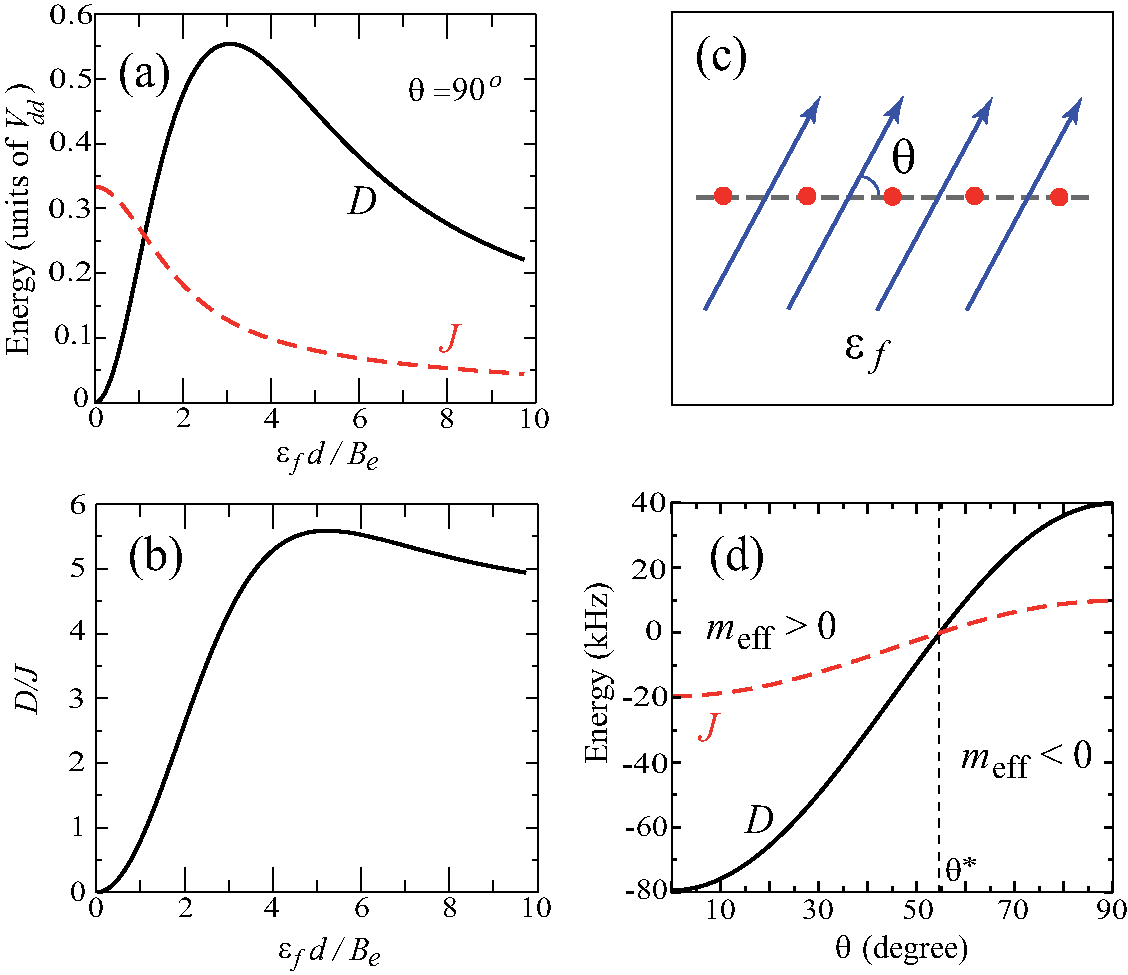
\includegraphics[scale=0.3]{Figure1FourPanels.pdf}
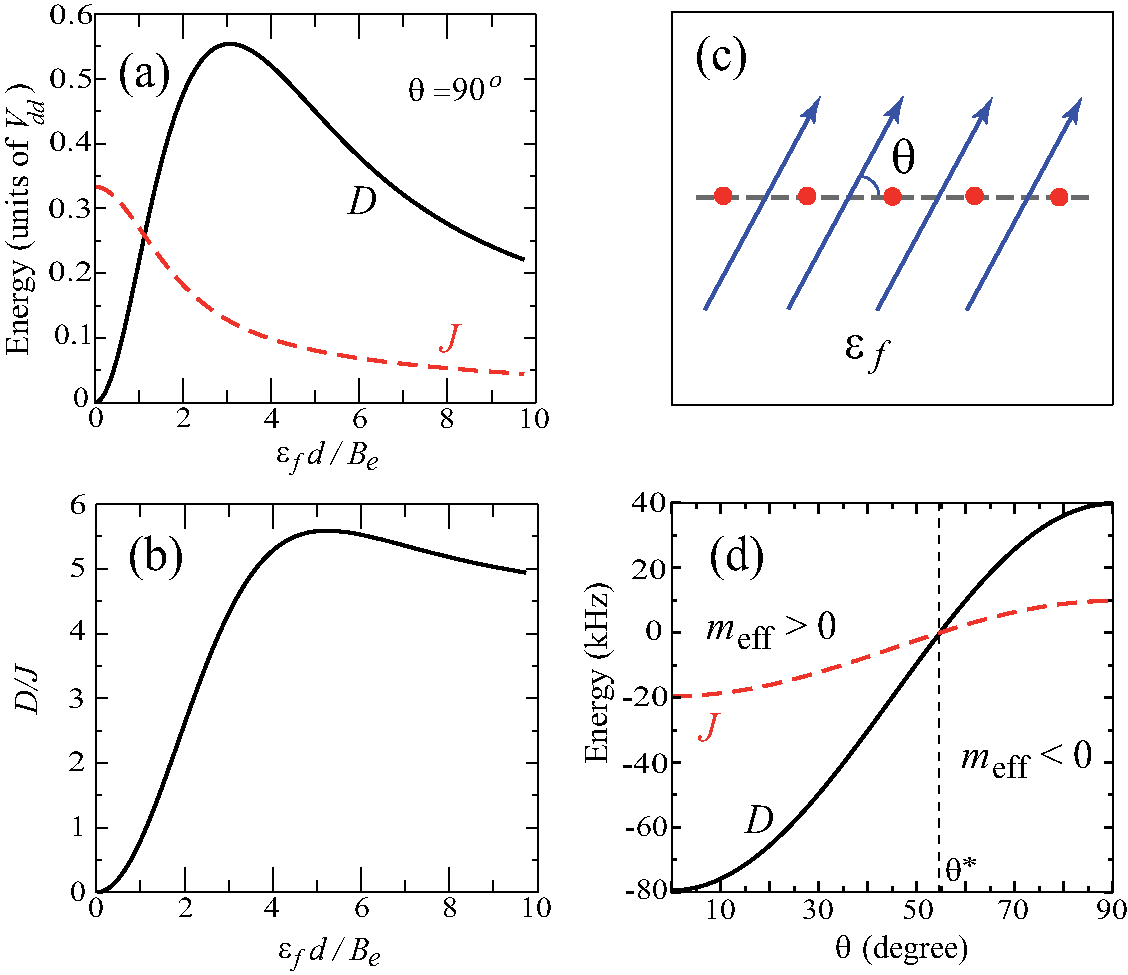
\includegraphics[width=\linewidth]{Figure1FourPanels.pdf}
\caption{ (a) The parameters $D$ and $J$ (in units of $V_{dd} = d^2/a^3$) as functions of the electric field strength.
 (b) The ratio  $D/J$ as a function of the electric field strength. The field is perpendicular to the intermolecular axis.
For LiCs molecules possessing the dipole moment $d$=5.529~Debye, the value ${\cal E}_f d/B_e = 1$ corresponds to
 ${\cal E}_f = 2.12$ kV/cm. (c) Schematic depiction of the angle $\theta$ between the field (represented by blue
 arrows) and the molecular array (represented by red dots). (d) $D$ and $J$ for a 1D array of LiCs molecules separated
 by 400 nm as functions of $\theta$ for ${\cal E}_f = 6$ kV/cm.
} \label{fig:HowDJChanges}
\end{figure}


\begin{figure}[htbp]
\centering
%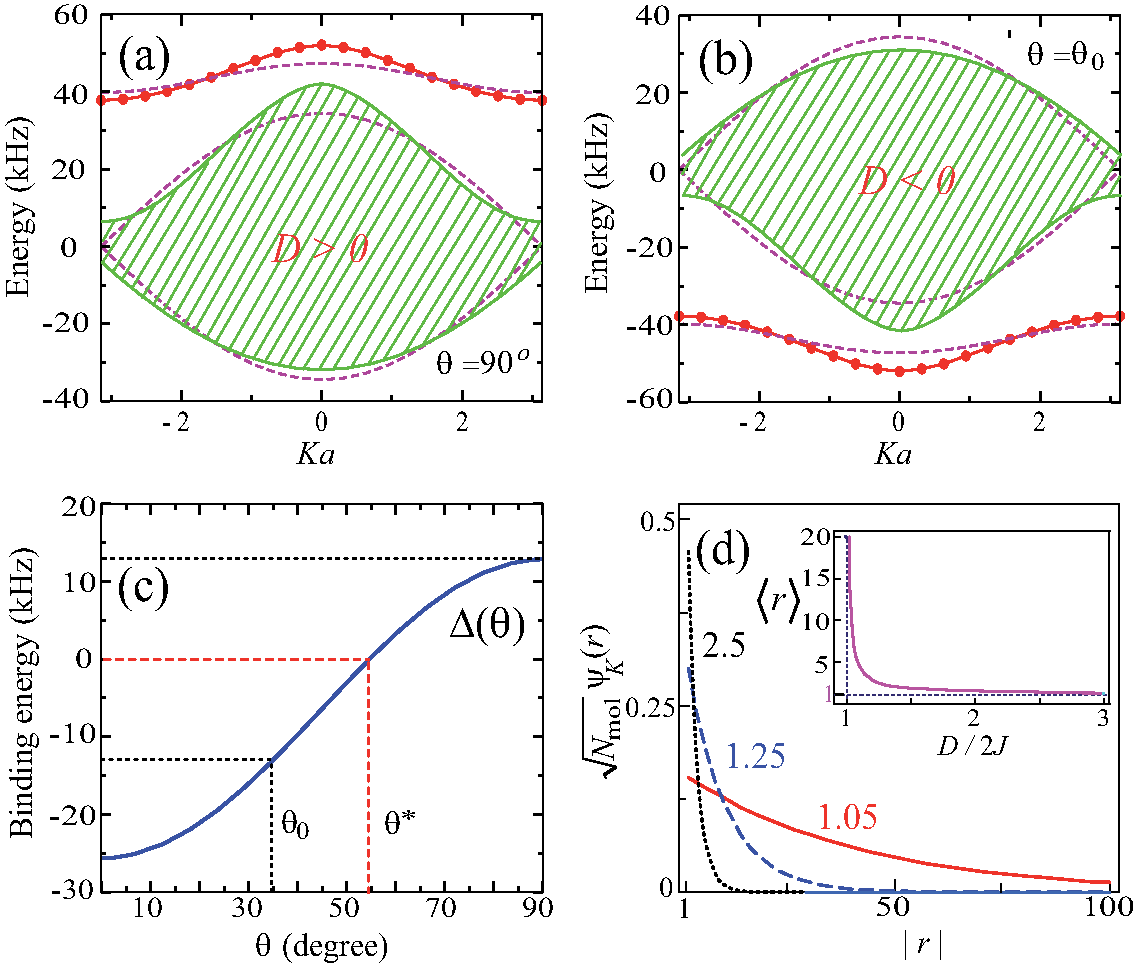
\includegraphics[scale=0.3]{FigureBiexciton.pdf}
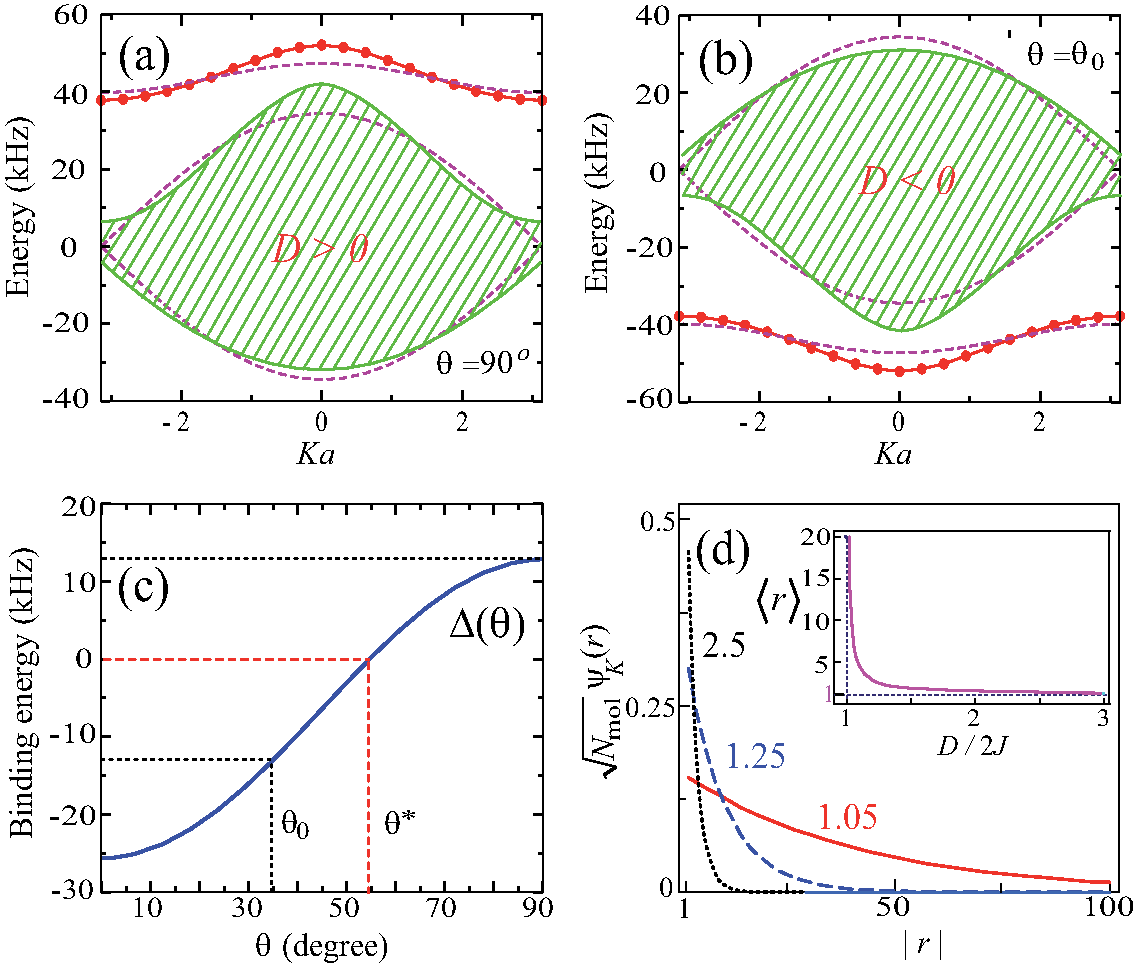
\includegraphics[width=\linewidth]{FigureBiexciton.pdf}
\caption{(a) and (b): Two-excitation spectra of a 1D array of LiCs molecules on an optical lattice: NNA
(dashed lines) and exact solutions (solid lines). The shaded regions encapsulate the bands of the continuum 
two-exciton states. (c)$\theta$-dependence of the biexciton binding energy $\Delta$. The electric field magnitude is
 6.88 kV/cm, $\theta_0 = \arccos \sqrt{2/3}$, $\theta^\ast = \arccos \sqrt{1/3}$. (d) Biexciton wave function vs the
 lattice site separation $|r|=|n-m|$ of the two excitations for $K=0$. Inset: Mean width of the biexciton wave function
 $\langle r \rangle$ calculated as the width of $\psi^{2}_{K}(r)$ at half maximum. Numbers at each curve indicate the
 value of $D/2J$.}
\label{fig:biexcitonSpectrum}
\end{figure}


For molecules in an optical lattice, the magnitudes of $J$ and $D$ depend on the strength of the applied electric field
 and the angle between the field and the molecular array  ($\theta$) (see \autoref{fig:HowDJChanges} (c) ).  We
 calculate these parameters for a 1D array of $^1\Sigma$ polar molecules (such as alkali metal dimers produced in
 ultracold molecule experiments) trapped on an optical lattice with the lattice separation $a = 400$ nm.
 \Autoref{fig:HowDJChanges} (b)
 shows that for a fixed angle $\theta$ the ratio $D/J$ increases as the electric field magnitude increases. 
For LiCs molecules, the condition (\ref{biexc-formation}) is satisfied for electric fields $>3.6$~kV/cm. Note that the
 ratio $D/J$ is independent of $\theta$. 

 Frenkel excitons are quasiparticles characterized by an effective mass ($m_{\rm eff}$). The sign of $J$ determines the
 sign of the  effective mass \cite{felipe}: negative $J$ corresponds to positive $m_{\rm eff}$ and vice versa (see
 \autoref{fig:HowDJChanges} (d) ). Due to the linearity of the Schr\"{o}dinger equation, a positive potential is
 attractive for particles with negative mass, just like a negative potential is attractive for particles with positive mass. 
 Because the sign of $J$ and $D$ is the same (and consequently the signs of $D$ and $m_{\rm eff}$ are opposite), the
 dynamical interaction (\ref{dynamical}) between excitons in this system is attractive.


To demonstrate the formation of the biexciton and calculate the biexciton energy, we diagonalize the Hamiltonian
 $\hat{H}_{\rm exc} + \hat{H}_{\rm dyn}$ for a one-dimensional array of $N_{\rm mol} = 501$ LiCs molecules. The
 matrix of the Hamiltonian is evaluated by expanding the biexciton states as 
\begin{eqnarray}
| \Psi_b(K) \rangle &=& \sum_{\substack{k_1 + k_2 = K \\ k_1 \ge k_2}} C_{k_1, k_2} \ket{k_1, k_2} \nonumber \\
&=&\sum\limits_{k \geq 0} C_k^K \ 
| \hat{P}^\dag(K/2 + k)  \hat{P}^\dag(K/2
- k) \rangle,
\label{wave-function} 
\end{eqnarray}
where $K = k_1+k_2$ and $k = (k_1 - k_2)/2$, and $k_1$ and $k_2$ denote the wavevectors of the interacting
 excitons. The Hamiltonian matrix is diagonalized numerically for fixed values of $K$, which is conserved.
 \Autoref{fig:biexcitonSpectrum} shows that for $\theta = 90^o > \theta^*=\arccos(1/\sqrt{3})$ the biexciton energy is
 above the two-exciton continuum (binding for particles with negative mass), and for
 $\theta = \arccos \sqrt{2/3} <  \theta^*$ below it (binding for particles with positive mass). The binding energy of the
 biexciton changes sign at $\theta = \theta^*$. The biexciton wave function $\psi_{K}(r)$ is plotted in
 \autoref{fig:biexcitonSpectrum} (d). \Autoref{fig:HowDJChanges} and \autoref{fig:biexcitonSpectrum} thus illustrate
 that the biexciton binding energy and size can be tuned by varying the strength and orientation of the electric field. 
 


\section{Non-optical creation of biexcitons} 
The possibility of formation of Frenkel biexcitons has been proposed quite long ago \cite{efremov1973}. However, in 
contrast to the well-known Wannier-Mott biexcitons in semiconductors, Frenkel biexcitons in solid-state molecular
 crystal are very difficult to observe. 
We now explain the reasons. First, many molecular crystals, such as anthracene or naphthalene,  possess inversion
 symmetry. In these crystals, the constant $D$ as defined in the line after \autoref{dynamical} must vanish and 
\autoref{biexc-formation} is not satisfied. Second, it is difficult to excite biexciton states optically: it was shown
 in Ref.\cite{Ezaki1994} that the oscillator strength for the photon-induced transitions to the biexciton state must
 decrease with the increasing binding energy of the biexcitons. Therefore, two-photon excitation can only produce
 unstable weakly bound biexcitons. Third, excitons in molecular crystals decay via bimolecular annihilation processes
 into higher-energy states and subsequent relaxation accompanied by emission of phonons. This process is prohibited
 by conservation of energy in an optical lattice with diatomic molecules. \Autoref{fig:HowDJChanges}  demonstrates
 that the first obstacle can be removed by tuning 
the electric field. To overcome the second obstacle, we propose a non-optical method of populating deeply bound
 biexciton states based on the unique structure of $^1\Sigma$ polar molecules. 
As zero electric field the rotational states $|g\rangle$ and $|e\rangle$ are separated by the energy 
$\Delta \epsilon_{e - g}= 2 B_e$, while the energy separation between state $|e\rangle$ and the next rotationally
 excited state $|f\rangle \equiv |N=2, M_N = 0\rangle$ is equal to $\Delta \epsilon_{e- f}=4B_e$. As the electric field
 increases, $\Delta \epsilon_{e - g}$ increases faster than $\Delta \epsilon_{e - f}$ (see \autoref{fig:rotationalEnergy}).
When ${\cal E}_f d/B_e \simeq 3.24$ (corresponding to ${\cal E}_f \simeq 6.88$ kV/cm for LiCs), 
$\Delta \epsilon_{f - g} = 2 \Delta \epsilon_{e - g}$. At electric fields near this magnitude, two 
$| g \rangle \rightarrow | e \rangle$ excitons can undergo the transition to the $|f \rangle$ state, and, inversely, 
the $|g \rangle \rightarrow |f\rangle$ excitation can produce a pair of $|g\rangle \rightarrow |e \rangle$ excitons or a
 biexciton state depicted in \autoref{fig:biexcitonSpectrum}. The coupling between states $| e \rangle$ and $| f \rangle$ is
$\hat{H}_{12} = \sum\limits_{n \neq m} M(n-m) \hat{R}_n  \hat{P}_n^\dag
\hat{P}_m^\dag$, where $M(n-m) = \langle e_{n},e_{m} | V_{dd}(n-m) | f_{n},g_{m}
\rangle$, and the operator $\hat{R}_n$ annihilates the $| f \rangle$
excitation in lattice site $n$. The total Hamiltonian describing this three-level 
system is $\hat{H}_{g-e-f} = \hat{H}_{\rm exc} + \hat{H}_{\rm dyn} +  \hat{H}_2 + \hat{H}_{12}$, where
$\hat{H}_2 = E_f \sum\limits_n \hat{R}_n^\dag \hat{R}_n   + \sum\limits_{n,m \neq n} J_{g-f}(n-m) \hat{R}_n^\dag \hat{R}_m $ and $J_{g-f}(n-m) = \langle g_{n},f_{m} | V_{dd}(n-m) | f_{n},g_{m} \rangle$.

\begin{figure}[ht]
\centering
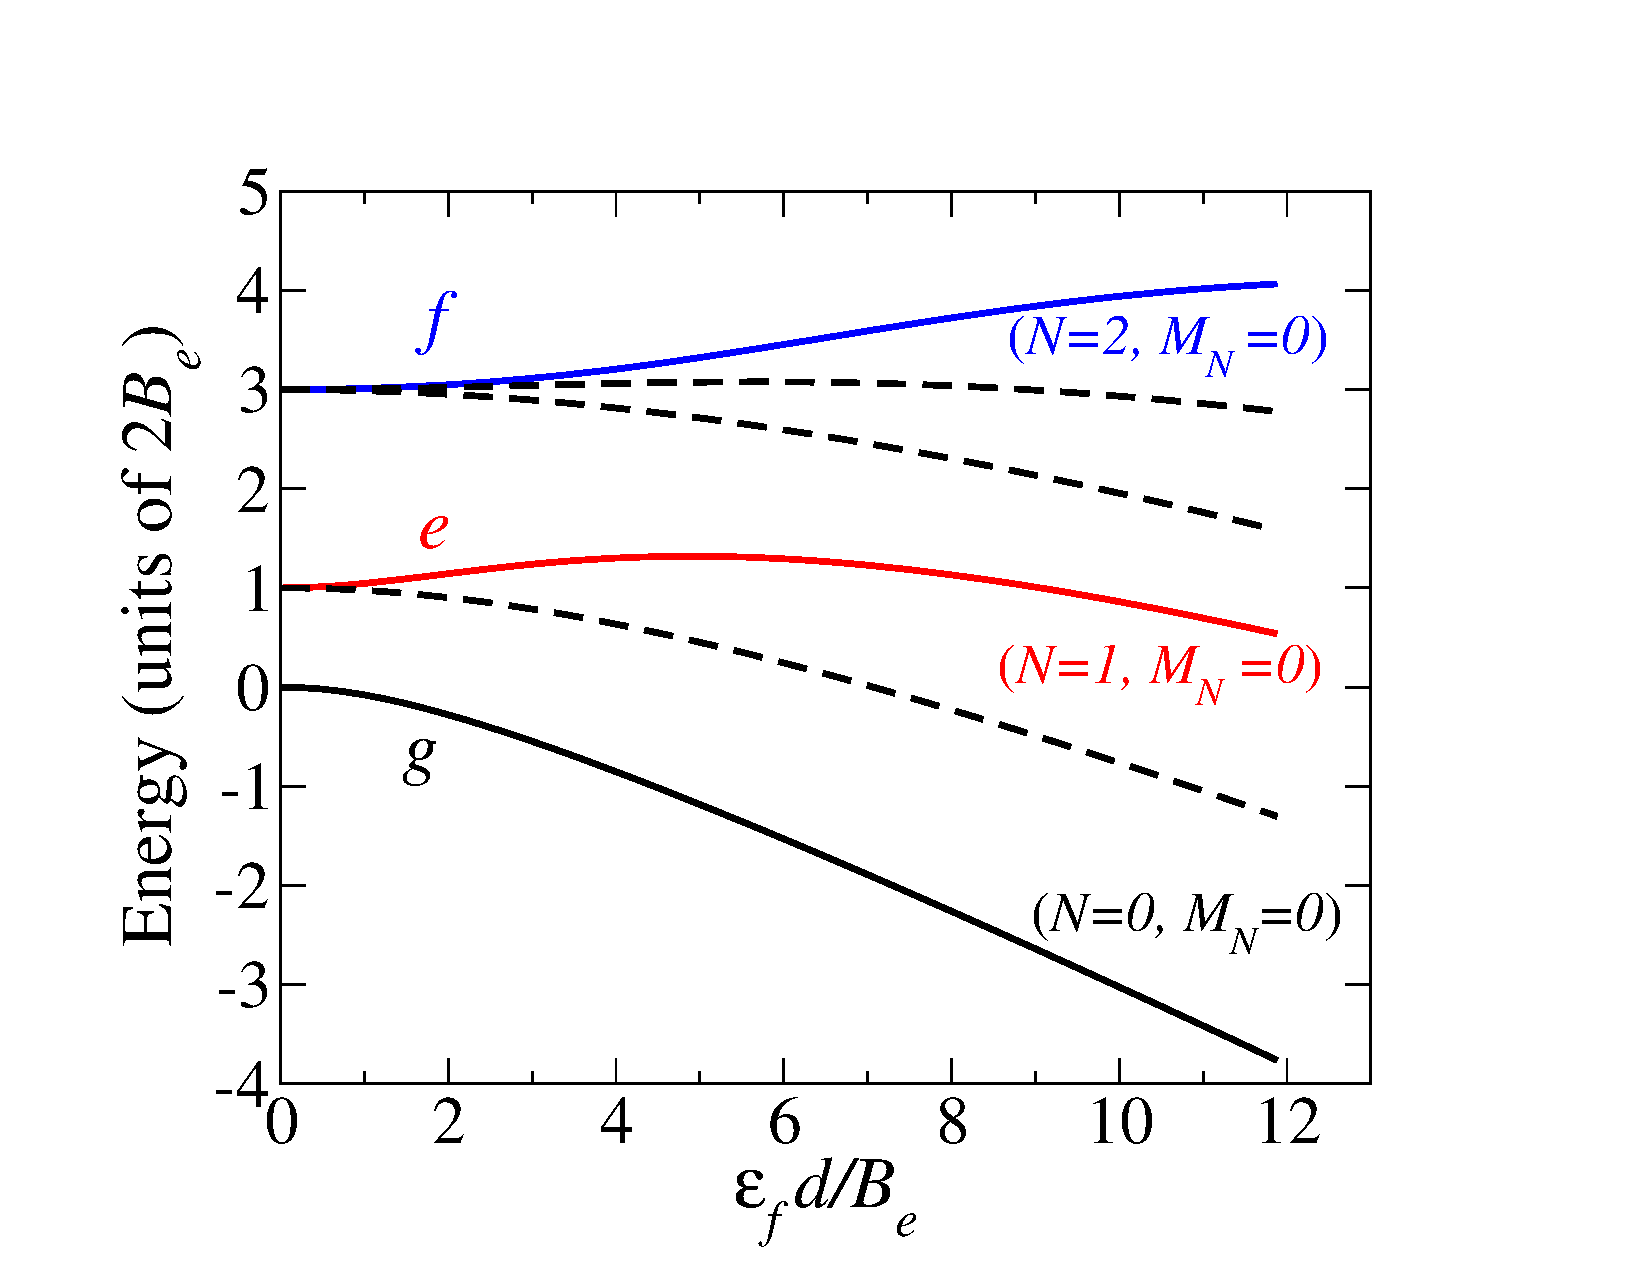
\includegraphics[width=\linewidth]{Figure3.pdf}
\caption{The energies of rotational levels as functions of the strength of the DC field. The dashed lines represent
other rotational states with $M_{N} \neq 0$. 
}
\label{fig:rotationalEnergy}
\end{figure}

\begin{figure}[htbp]
\centering
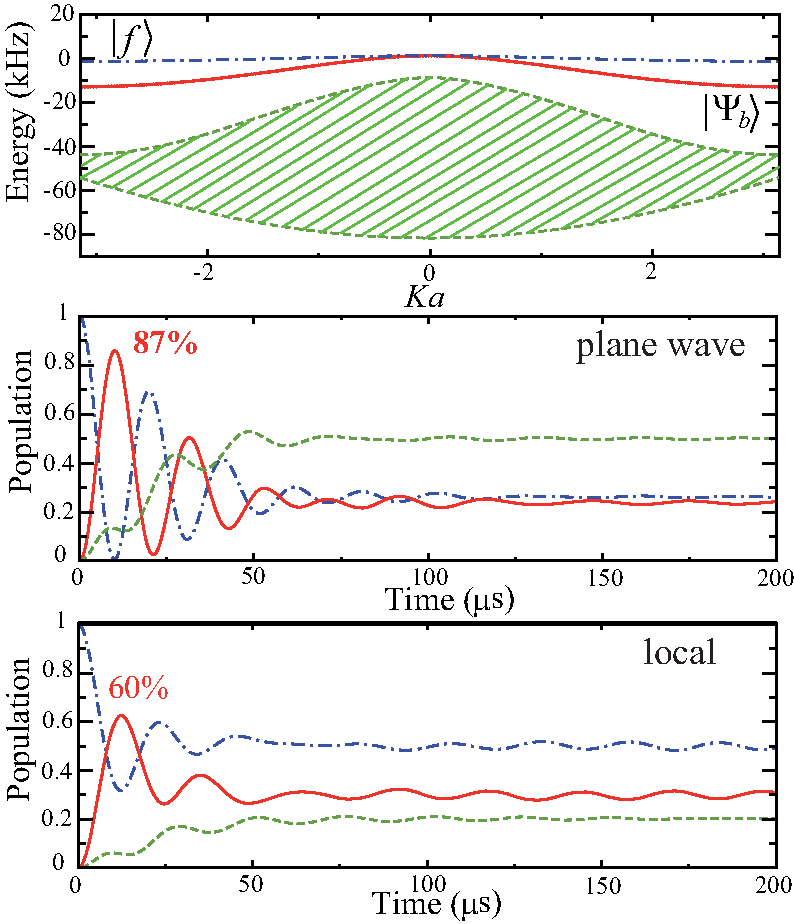
\includegraphics[scale=0.8]{Figure4.pdf}
%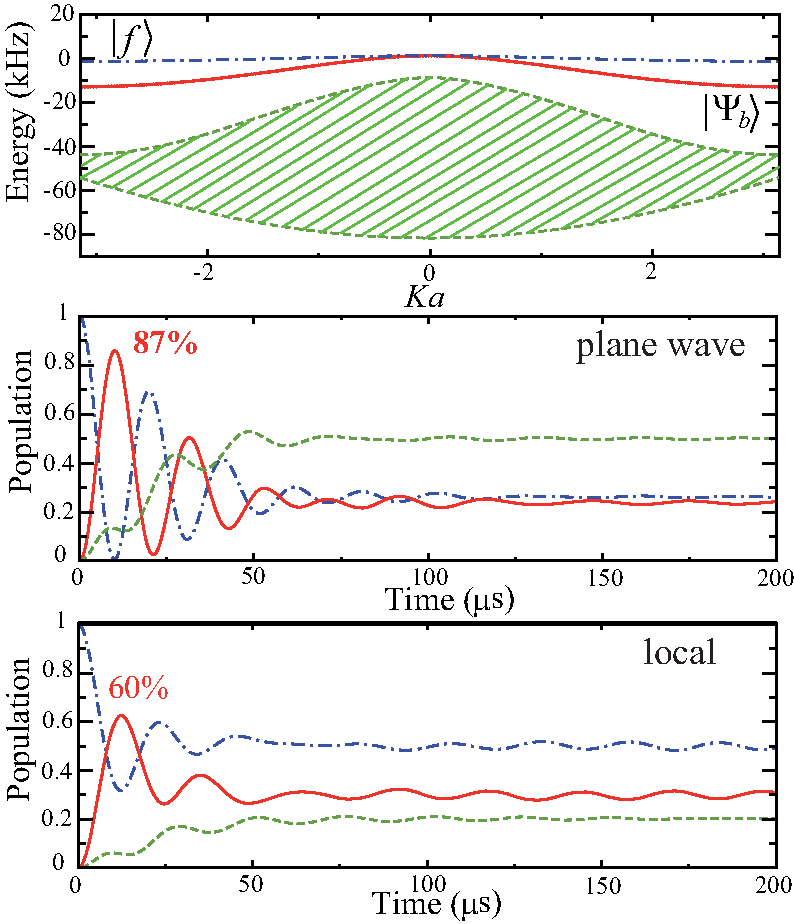
\includegraphics[width=\linewidth]{Figure4.pdf}
\caption{Population dynamics for the transition from $|g\rangle \to |f\rangle$ exciton (middle panel) and from an $f$
 state localized on a single molecule (lower panel) to coherent $|g\rangle \to |e\rangle$ excitons and biexcitons. The
 green dashed curves denote the population accumulated in the pairs of non-bound $|g\rangle \to |e\rangle$ exciton
 states, the red solid curves the biexciton state and the blue dot-dashed curves the $f$ state. The shaded region in the
 upper panel encapsulates the band of the continuum two-exciton states. The calculation is for a 1D ensemble of
 $N_{mol}=501$ LiCs molecules on an optical lattice with lattice separation a = 400 nm. The electric field of magnitude
 6.88 kV/cm is perpendicular to the molecular array.}
\label{fig:populationDynamics}
\end{figure}



In order to calculate the probability of the population transfer from state $f$ to the biexciton state, we solve the
 time-dependent Schr\"{o}dinger equation with the Hamiltonian $\hat{H}_{g-e-f}$ evaluated in the basis of products of
 the eigenstates of $\hat{H}_{\rm exc} + \hat{H}_{\rm dyn}$ and the eigenstates of $\hat{H}_2$. This leads to coupled
 differential equations:
\oneline{
i\hbar\mathbf{\dot{C}} = \mathbf{H}\mathbf{C} \ , \label{eqn:matrixDifferentialEqs}
} 
where $\mathbf{C}$ is a vector that represents a wavefunction in the basis set and $\mathbf{\dot{C}}$ is its derivative
with respect to time. Since the total Hamiltonian $\mathbf{H}$ is time-independent, we can make a basis-set 
transformation to diagonalize $\mathbf{H}$
\oneline{
\mathbf{U^{T}} \mathbf{H} \mathbf{U} = \mathbf{D} \ , 
}
 so that $\mathbf{C}$ in the new basis set can then be solved by direct
 integration and then $\mathbf{C}$ in the original basis set can be found by the inverse basis-set transformation. 
Mathematically speaking, we multiply $\mathbf{U^{T}}$ on both sides of \autoref{eqn:matrixDifferentialEqs} and 
obtain
\multiline{
i\hbar\mathbf{U^{T}} \mathbf{\dot{C}} &=& \mathbf{U^{T}} \mathbf{H} \mathbf{U} \mathbf{U^{T}}\mathbf{C} \ , \label{eqn:matrixDifferentialEqsModified}
}
where $ \mathbf{U} \mathbf{U^{T}} = \mathbf{I}$ has been used. Let's define
\oneline{
\mathbf{A} \equiv \mathbf{U^{T}} \mathbf{C} \ , \label{eqn:changeBasis}
}
then
\oneline{
\mathbf{\dot{A}} =  \mathbf{U^{T}} \mathbf{\dot{C}} 
}
because $\mathbf{H}$ is time-independent and $\mathbf{U^{T}}$ must be time-independent too.  
So \autoref{eqn:matrixDifferentialEqs} can be rewritten as
\oneline{
i\hbar \mathbf{\dot{A}} = \mathbf{D} \mathbf{A} \ , 
}
which can solved easily by direct integration:
\oneline{
\mathbf{A}(t) = e^{-\frac{i}{\hbar} \mathbf{D} \; t} \mathbf{A}(0) \ .  \label{eqn:solForA}
}
Substituting \autoref{eqn:changeBasis} to \autoref{eqn:solForA}, we get
\oneline{
\mathbf{C}(t) = \mathbf{U} e^{-\frac{i}{\hbar} \mathbf{D} \; t} \mathbf{U^{T}} \mathbf{C}(0) \ ,  \label{eqn:solForC}
}
where $\mathbf{D}$ is a diagonal matrix whose non-zero elements are eigenvalues of $\mathbf{H}$, and each
column of $\mathbf{U}$ is an eigenvector of $\mathbf{H}$. Therefore, given the eigenvalues and eigenvectors of the
total Hamiltonian and the initial wavefunction $\mathbf{C}(0)$, the wavefunction $\mathbf{C}(t)$ at any time $t$ can
be calculated from \autoref{eqn:solForC}. In our numerical calculations, we use subroutines from the LAPACK library
to calculate the eigenvalues and eigenvectors of the matrix. 


The magnitude of $J_{g-f}$ is about ten times smaller than $J$.
 In the absence of decoherence, the $| g \rangle \rightarrow | f \rangle$ excitation gives rise to the Frenkel exciton and
 the transition from the $f$ states to 
 the biexciton state is a coherent exciton--exciton transition. In the presence of decoherence, the exciton states
 become localized. If the decoherence rate is larger than $J_{g-f}/h$, but smaller than $J/h$, the
 $| g \rangle \rightarrow | f \rangle$ excitation is localized, while the biexciton states remain coherent.
 \Autoref{fig:populationDynamics} presents the calculations of the population transfer probabilities for both
 scenarios. The results show that the biexciton states can be populated with high efficiency. The equilibrium
 populations (in the limit of large $t$) depend on the relative energies of the $f$ state, the biexciton bound state and
 exciton--exciton continuum states, which can be tuned by varying the electric field magnitude. 
The efficiency of the population transfer can be maximized if the electric field is detuned far away from resonance
 when the biexciton population oscillations reach the first maximum. Detuning the electric field to low magnitudes
 effectively decouples the $f$ state from the states in the $\{g,e\}$ subspace and interrupts the population dynamics.
 This corresponds to switching off the channel for bimolecular annihilation of excitons, which is one of the reasons of
 the biexciton population depletion in solids. We have confirmed that the calculations with electric fields $< 5.0$
 kV/cm yield no  noticeable population transfer. 

\section{Extension to exciton trimers}
\label{sec:trimers}
In \autoref{sec:biexciton}, it is shown that Frenkel rotational biexcitons exist under some conditions in optical lattices. 
Then the question arises naturally: if two excitons can bind together, what about three excitons? In this section, we
try to extend the method to handle the three-exciton case and answer the question about exciton trimers. 

Similar to the case of biexciton, we define a three-exciton wavefunction in site representation
\oneline{
\ket{\Psi} = \sum_{n_1, n_2, n_3} C_{n_1, n_2, n_3}\pd{n_1}\pd{n_2}\pd{n_3} \ket{0} \ , 
}
and start from the Sch{\"o}dinger equation with the same Hamiltonian 
$\hat{H} = \hat{H}_{\rm exc} + \hat{H}_{\rm dyn} $
\oneline{
\hat{H} \ket{\Psi} = E_{\rm trimer}  \ket{\Psi}  \ . \label{eqn:schrodingerTrimer}
}
Since two excitations can't sit at the same molecule, we have the constraint on $C_{n_1, n_2, n_3}$:
\oneline{
C_{n_1, n_2, n_3} = 0 \;\; \mbox{\rm if $n_1 = n_2$ or $n_2 = n_3$ or $n_1 = n_3$} \ . \label{eqn:trimerConstraint}
} 
After similar derivations as we did for the biexciton case, \autoref{eqn:schrodingerTrimer} and
 \autoref{eqn:trimerConstraint} leads to
\multiline{
&&\left[3 E _0 D(n_1-n_2) + D(n_1-n_3) + D(n_2 - n_3) - E_{\rm trimer} \right] C_{n_1, n_2, n_3} \nonumber \\
&& \hspace{0.5cm} + \sum _n\left[J(n- n_1)C_{n, n_2, n_3} + J(n-n_2)C_{n_1, n, n_3} + J(n-n_3 )C_{n_1, n_2, n}\right] \nonumber \\
&& = 2\delta _{n_1,n_2}\sum _{n}J(n_1-n)C_{n, n_2, n_3} + 2\delta _{n_2, n_3}\sum _{n}J(n_2 -n)C_{n_1, n, n_3} \nonumber \\
&&  \hspace{0.5cm} + 2\delta _{n_1,n_3}\sum _{n} J(n_3 -n)C_{n_1, n_2, n}  \ . \nonumber \\ \label{eqn:schrodingerTrimerSite}
}
Note the equation can't be used to determine the values of $C_{n_1, n_2, n_3}$ when any two of $n_1$, $n_2$, and $n_3$ are equal. Using the following Fourier transform
\oneline{
C_{n_1, n_2, n_3} = \frac{1}{\left(\sqrt{N_{\rm mol}}\right)^3}\sum_{k_1, k_2, k_3} C(k_1, k_2, k_3) e^{i (k_1 n_1 + k_2 n_2 + k_3 n_3) }
}
we can transform \autoref{eqn:schrodingerTrimerSite} to 
\multiline{
&&\frac{1}{N_{\rm mol}}\sum _{q}\Tilde{D}(q) \left[C(k_1-q, k_2+q, k_3)+C(k_1 -q, k_2, k_3+q)+C(k_1,k_2-q,k_3+q)\right] \nonumber \\
&& \hspace{0.5cm} + \left[\epsilon(k_1)+ \epsilon(k_2)+ \epsilon(k_3)-E _{\rm trimer}\right]C(k_1, k_2, k_3) \nonumber \\ 
&&=\frac{2}{N_{\rm mol}}\sum _{q}\left[ \Tilde{J}(k_1-q)C(k_1-q,k_2+q,k_3)+\Tilde{J}(k_2-q)C(k_1,k_2-q,k_3+q) \right. \nonumber \\
&& \left.  \hspace{1.5cm} + \Tilde{J}(k_3-q)C(k_1+q,k_2+q,k_3-q)\right] \ , \label{eqn:threeBodyEq}
}
which can be written as an eigenvalue problem
\oneline{
\sum_{k_1^{'} + k_2^{'} + k_3^{'} = K} \mathbf{A}_{k_1 k_2 k_3; k_1^{'} k_2^{'} k_3^{'}} C(k_1^{'}, k_2^{'}, k_3^{'}) = E _{\rm trimer} C(k_1, k_2, k_3) \ , \label{eqn:trimerMatrixEq}
} 
where 
\multiline{
\mathbf{A}_{k_1 k_2 k_3; k_1^{'} k_2^{'} k_3^{'}} &=& \delta_{k_1, k_1^{'}} \delta_{k_2, k_2^{'}} \delta_{k_3, k_3^{'}} \left[ \epsilon(k_1) + \epsilon(k_2) + \epsilon(k_3)\right]  \nonumber \\
&& + \frac{1}{N_{\rm mol}} \left\{ \delta_{k_1, k_1^{'}} \left[ \Tilde{D}(k_2 - k_2^{'}) -2 \Tilde{J}(k_2^{'})  \right] \right. \nonumber \\
&&\hspace{1.5cm} +  \delta_{k_2, k_2^{'}} \left[ \Tilde{D}(k_3 - k_3^{'}) -2 \Tilde{J}(k_3^{'})  \right] \nonumber \\
&&\hspace{1.5cm} \left. +  \delta_{k_3, k_3^{'}} \left[ \Tilde{D}(k_1 - k_1^{'}) -2 \Tilde{J}(k_1^{'})  \right] \right\} \ .
}
The above equations clearly show that only those $C(k_1, k_2, k_3)$'s whose wavevectors add up to a fixed $K$
 are coupled to each other. Therefore, the eigenvalues for each value of $K$ can be calculated independently.
However, \autoref{eqn:trimerMatrixEq} is not the whole story. Since we have assumed that $C_{n_1, n_2, n_3} = 0$
when any two of $n_1, n_2, n_3$ are equal, we need to take care of the constraint when solving
 \autoref{eqn:trimerMatrixEq}. 

Let's see what does the constraint on $C_{n_1, n_2, n_3}$ imply for $C(k_1, k_2, k_3)$. Assuming $k_3$ is fixed, we have
\multiline{
\sum_{k_1 + k_2 = K - k_3} C(k_1, k_2, k_3) &=& \sum_{k_1}\sum_{n_1, n_2, n_3 }\frac{1}{\left( \sqrt{N_{\rm mol}}\right)^3} e^{i (k_1 n_1 + k_2 n_2 + k_3 n_3 )} C_{n_1, n_2, n_3} \nonumber \\
&=& \sum_{n_1, n_2, n_3 }\frac{1}{ \sqrt{N_{\rm mol}}} \left( \frac{1}{N_{\rm mol}}\sum_{k_1}e^{i k_1 (n_1 - n_2) }\right) e^{i (K - k_3 ) n_2} e^{i k_3 n_3} C_{n_1, n_2, n_3} \nonumber \\
&=&\sum_{n_1, n_2, n_3 }\frac{1}{ \sqrt{N_{\rm mol}}}  \delta_{n_1, n_2} e^{i (K - k_3 ) n_2} e^{i k_3 n_3} C_{n_1, n_2, n_3} \nonumber \\
&=&\sum_{ n_2, n_3 }\frac{1}{ \sqrt{N_{\rm mol}}} e^{i (K - k_3 ) n_2} e^{i k_3 n_3} C_{n_2, n_2, n_3} \nonumber \\
&=& 0 \ . \label{eqn:specificCondition}
}


Since the fixed wavector $k_3$ can be chosen arbitrarily, a condition similar to  \autoref{eqn:specificCondition} will
holds for a fixed $k_1$ and a fixed $k_2$ as well. This means:  for a particular $K$ if you add up all  
$C(k_1^{'}, k_2^{'}, k_3^{'})$ whose first (second or third) wavevector $k_1^{'} ( k_2^{'} \mbox{ or }  k_3^{'})$ equal to a fixed $k$, you will get zero. Thus we can add the zero
\multiline{
&&\frac{1}{N_{\rm mol}} \sum_{k_1^{'}, k_2^{'}, k_3^{'} } \left[ -2\Tilde{J}(k_2) \delta_{k_1^{'}, k_1} C(k_1^{'}, k_2^{'}, k_3^{'})  -2\Tilde{J}(k_3) \delta_{k_2^{'}, k_2} C(k_1^{'}, k_2^{'}, k_3^{'}) \right. \nonumber \\
&& \left. -2\Tilde{J}(k_1) \delta_{k_3^{'}, k_3} C(k_1^{'}, k_2^{'}, k_3^{'}) \right] = 0
}
 to the left hand side of \autoref{eqn:trimerMatrixEq} to produce a new equation
\oneline{
\sum_{k_1^{'} + k_2^{'} + k_3^{'} = K} \mathbf{B}_{k_1 k_2 k_3; k_1^{'} k_2^{'} k_3^{'}} C(k_1^{'}, k_2^{'}, k_3^{'}) = E _{\rm trimer} C(k_1, k_2, k_3) \ , \label{eqn:trimerMatrixEqSymmetric}
} 
where
\multiline{
\mathbf{B}_{k_1 k_2 k_3; k_1^{'} k_2^{'} k_3^{'}} &=& \delta_{k_1, k_1^{'}} \delta_{k_2, k_2^{'}} \delta_{k_3, k_3^{'}} \left[ \epsilon(k_1) + \epsilon(k_2) + \epsilon(k_3)\right]  \nonumber \\
&& + \frac{1}{N_{\rm mol}} \left\{ \delta_{k_1, k_1^{'}} \left[ \Tilde{D}(k_2 - k_2^{'}) -2 \Tilde{J}(k_2) -2 \Tilde{J}(k_2^{'})  \right] \right. \nonumber \\
&&\hspace{1.5cm} +  \delta_{k_2, k_2^{'}} \left[ \Tilde{D}(k_3 - k_3^{'}) -2 \Tilde{J}(k_3) -2 \Tilde{J}(k_3^{'})  \right] \nonumber \\
&&\hspace{1.5cm} \left. +  \delta_{k_3, k_3^{'}} \left[ \Tilde{D}(k_1 - k_1^{'}) -2 \Tilde{J}(k_1)-2 \Tilde{J}(k_1^{'})  \right] \right\} \ .
}
The advantage of \autoref{eqn:trimerMatrixEqSymmetric} over \autoref{eqn:trimerMatrixEq} is that the matrix
$\mathbf{B}$ is symmetric, which leads to easier diagonalization. 

 

\begin{figure}[htbp]
\centering
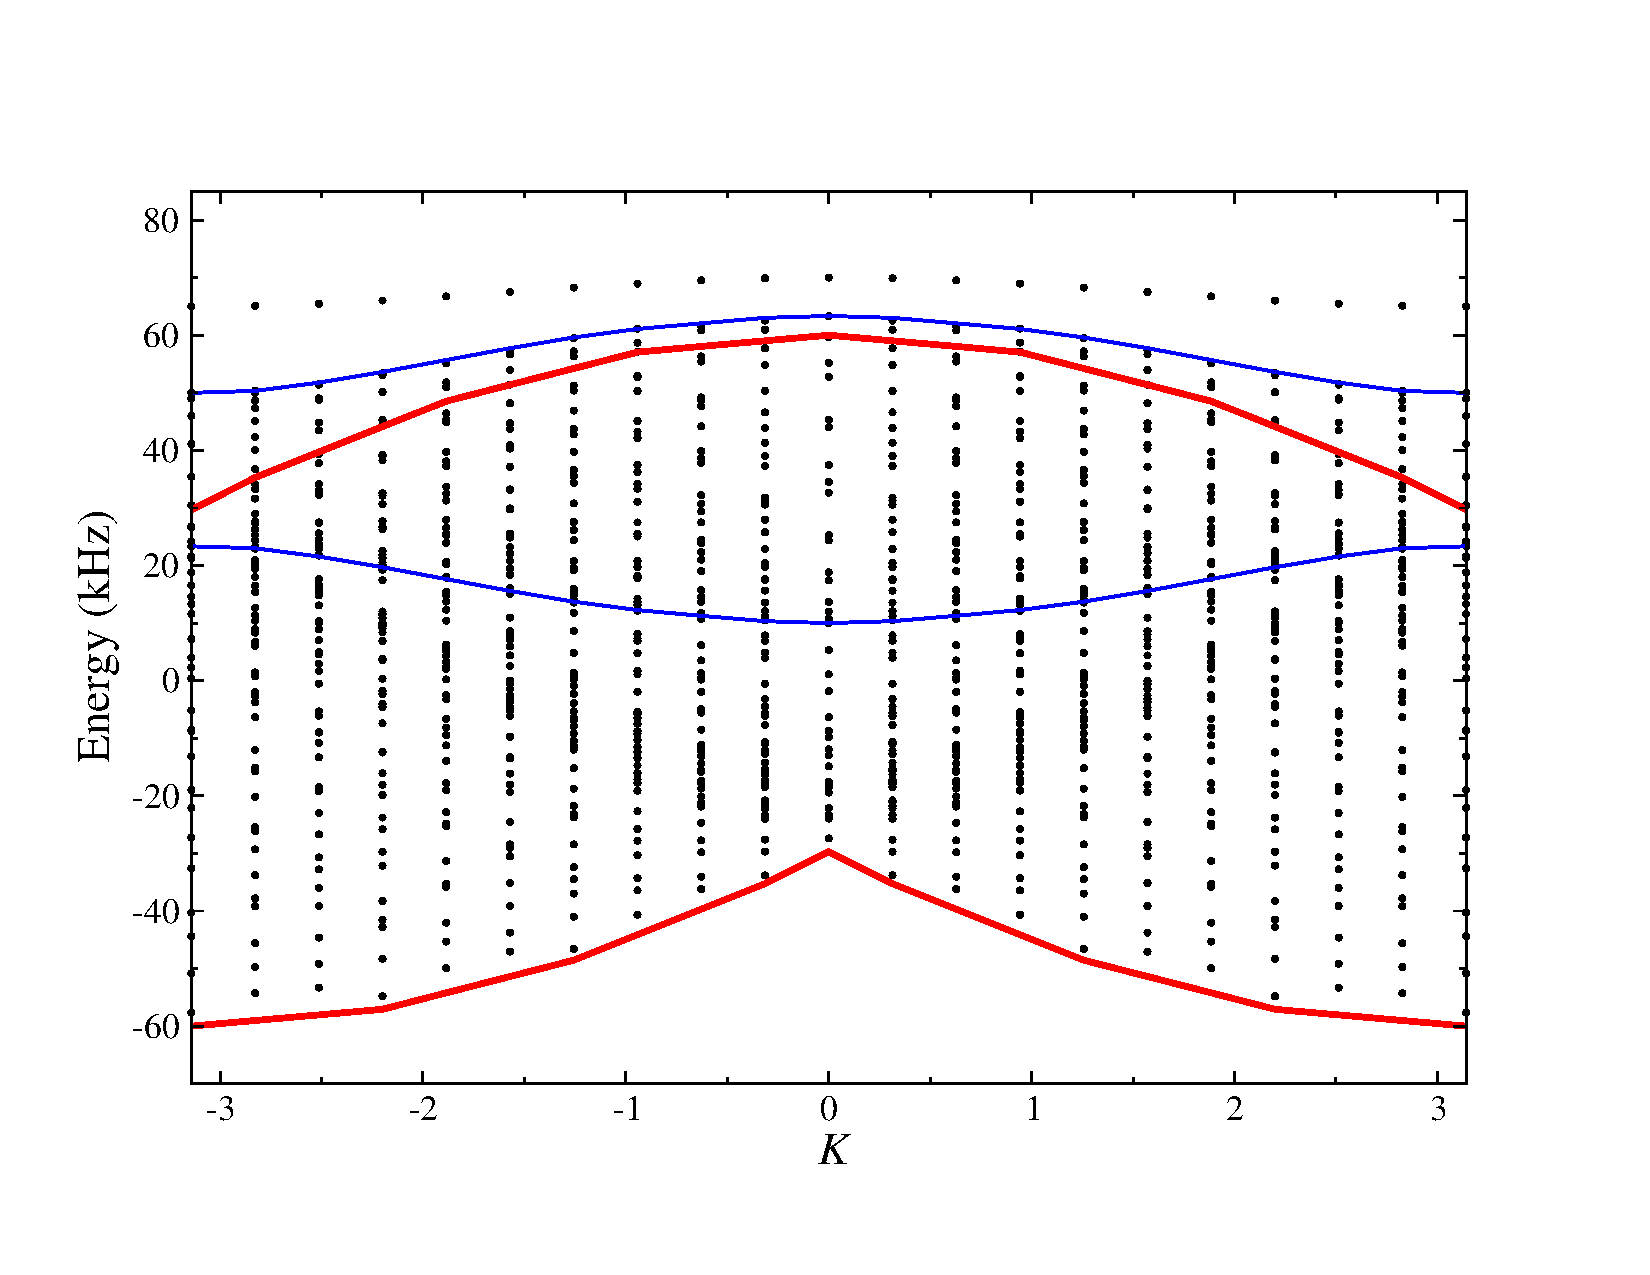
\includegraphics[width=\linewidth]{threeExcitons.pdf}
\caption{Three-excitation spectra of a 1D array of molecules on an optical lattice. The calculation is done for a
 system of 20 lattice sites with the hopping interaction $J =10$ kHz and the dynamic interaction $D =30$ kHz.
The black dots represent energies of all three-exciton states, the red curves denote the boundaries of  energy
 continuum of three free excitons, and the blue curves represent the boundaries of energy continuum for a biexciton 
plus a free exciton. 
   }
\label{fig:trimer}
\end{figure}


\section{Discussion} 
We have shown that rotational excitation of molecules trapped on an optical lattice gives rise to rotational excitons
 whose interactions can be controlled by an external electric field. The exciton--exciton interactions can be tuned to
 produce two-exciton bound states.  A biexciton is an entangled state of two Frenkel excitons. The creation of
 biexcitons as described in the previous section and tuning the electric field to the regime of zero binding energy can
 thus be used for the controlled preparation of entangled pairs of non-interacting excitons. In order to observe the
 biexcitons, one could measure correlations between the populations of the rotationally excited states of molecules in
 different lattice sites using the method proposed in Ref. \cite{demille}. 




The present work suggests several interesting questions. For example, it was recently shown that Frenkel excitons in
 shallow optical lattices can be coupled to lattice phonons, leading to polarons \cite{felipe-polarons}. Coupling a
 Frenkel biexciton to phonons would produce strongly interacting polarons. It would be interesting to explore if these
 interactions lead to the formation of bipolarons. 



We have repeated the calculations presented here for a system of three excitons and similarly observed the formation
 of three-exciton bound states. It would be interesting to explore the effect of tunable exciton--exciton interactions
 on excitation correlations, both as a function of $D/J$ and the density of excitations, to understand fundamental
 limits of exciton clustering \cite{exciton-cluster}. 


The creation of biexcitons with tunable binding energy and measuring quantum energy transport for different ratios
 $D/J$ can be used to study the effects of exciton--exciton entanglement on energy transfer in molecular aggregates
 \cite{photosynthesis-1,photosynthesis-2,photosynthesis-3}. The ability to tune exciton--exciton interactions can be
 used to explore the role of multiple excitation correlations on energy transfer in disordered systems (the confining
 lattice potential can be tilted or the molecules can be perturbed by a disorder potential produced by an
 inhomogeneous electric field).
  






\chapter{Non-adiabatic control of quantum energy transfer in ordered and disordered arrays}
\label{ch:wave packet}

An elementary excitation in an aggregate of coupled particles
generates a collective excited state. We show that the dynamics of
these excitations can be controlled by applying a transient external
potential which modifies the phase of the quantum states of the 
individual particles. The method is based on an interplay of
adiabatic and sudden time scales in the quantum evolution of the many-body states. We show that
specific phase transformations can be used to accelerate or
decelerate quantum energy transfer and spatially focus delocalized
excitations onto different parts of  arrays of quantum
particles. {We consider possible experimental implementations of
the proposed technique and study the effect of disorder due to
the presence of impurities on its fidelity. {We further show
that the proposed technique can allow control of energy transfer  in completely disordered systems.}}


\section{Introduction}
\label{sec:energyTransferIntro}

The experiments with ultracold atoms and molecules trapped in optical lattices have opened a new frontier of 
condensed-matter physics research. The unique properties of these systems -- in particular, large ($>$ 400 nm) 
separation of lattice sites, the possibility of tuning the tunnelling amplitude of particles  between lattice sites by
 varying the trapping field and the possibility of controlling interparticle interactions with external electric or 
magnetic fields -- offer many exciting applications ranging from quantum simulation of complex lattice models 
\cite{Kohl2005, Barnett2006, micheli2006, Brennen2007, Buchler2007, McKay2008, Jordens2008, Schneider2008, 
Carr, Carr2, Trefzger2010, Kestner2011, gorshkov, gorshkov2} to the study of novel quasi-particles \cite{biexcitons}
 that cannot be realized in solid-state crystals.
 In the limit of strong trapping field,  each site of an optical lattice is populated by a fixed number of ultracold atoms
 or molecules. 
Such states can be produced with either bosonic or fermionic particles \cite{Greiner2002, Jordens2008}. Here, we consider
 an optical lattice fully or partially filled with one particle per lattice site, and assume that tunnelling between lattice
 sites is completely suppressed. Such an array can be thought of as a prototype  of a  system,
 in which a single lattice site (or a small number of lattice sites) can be individually addressed
by an external field of a focused laser beam. This can be exploited for engineering the properties of quantum 
many-body systems by changing the energy of particles in individual lattice sites \cite{our-2012-prl}.




In the present work, we consider the generic problem of energy transfer -- i.e. the time evolution of an elementary  
quantum excitation -- in such a system. In particular, we explore the possibility of controlling energy transfer through
 an array of coupled quantum monomers by applying monomer-specific external perturbations. This is necessary for 
several applications. First, collective excitations in molecular arrays in optical lattices have been proposed as 
high-fidelity candidates for quantum memory \cite{peter-rabl, peter-rabl2}.  The ability to manipulate collective excitations is necessary
 for building scalable quantum computing networks \cite{quantum-computing}. 
Second, ultracold atoms and 
molecules in optical lattices can be perturbed by a disorder potential with tunable strength 
\cite{anderson-localization-of-ultracold-atoms}. Engineering localized and delocalized excitations in such systems 
can be used to investigate the role of disorder-induced perturbations  on quantum energy transfer, a question of
 central importance for building efficient light-harvesting devices \cite{solar-cell}.
 Third, the possibility of controlling energy transfer in an optical lattice with ultracold atoms or molecules can
 be used to realize inelastic scattering processes with both spatial and temporal control. Finally, control over energy
transfer in quantum systems can be used for studying condensed-matter excitations and energy transport without 
statistical averaging.

An excitation of a coupled many-body system generates a wave packet representing a coherent superposition of 
single-particle excitations. The method proposed here is based on shaping such many-body wave packets by a series
 of sudden perturbations, in analogy with the techniques developed for strong-field alignment and orientation of 
molecules in the gas phase \cite{alignment-review}. Alignment is used in molecular imaging experiments and
 molecular optics \cite{alignment-review, imaging1, imaging2, imaging3}, and is predicted to provide control over 
mechanical properties of molecular scattering \cite{averbukh-AlignedInteractions, averbukh-AlignedInteractions2}. 
Here, we consider the use of similar techniques for controlling quantum energy transfer in an  interacting
 many-body system.
 When applied to a completely ordered system, the proposed method is reminiscent of the techniques used to 
move atoms in optical lattices, where a uniform force is applied for a short period of time \cite{denschlag2002}. 
The conceptual difference comes from the fact that in the present case the momentum is acquired by a 
quasi-particle -- a collective excitation distributed over many monomers. During the subsequent evolution, 
the particles do not move -- rather, the excitation is transferred from one monomer to another. In order to control
 such excitations, we exploit an interplay of the adiabatic and sudden time scales, which correspond to
 single-monomer and multi-monomer evolution. We also exploit the wave-like nature of the excitation wave function
 to draw on the analogy with wave optics. This analogy, too, is not complete due to the discrete nature of the lattice.

In order to emphasize the generality of the proposed method, we formulate the 
problem in terms of the general Hamiltonian parameters. We then describe in detail how the required external 
perturbations can be realized in experiments with ultracold atoms and molecules. The possibility of using rotational 
excitations in molecular arrays is particularly interesting due to the long lifetime of rotationally excited states. 
Electronic excitations of atoms in an optical lattice may also give rise to collective excitations \cite{Zoubi1}. However, the 
lifetime of these excited states is limited by fast spontaneous emission \cite{electronic-exciton1, electronic-exciton2}. We propose a mechanism for 
suppressing spontaneous decay by tailoring the properties of the excitation wave packets. 


The paper has the following structure. \Autoref{sec:phaseKicking} and \autoref{sec:focusing} present the results in terms of the general 
Hamiltonian parameters.  \Autoref{sec:excitationAtomMolecule} addresses the particular case of ultracold atoms and molecules.
\Autoref{sec:controlEnergyTransfer} discusses controlled energy transfer in systems with, specifically, 
dipole - dipole interactions. \Autoref{sec:energyTransferVacancy} considers the effects of lattice vacancies on the possibility of controlling 
energy transfer and \autoref{sec:focusingStrongDisorder} extends the proposed technique to
control of excitation dynamics in strongly disordered arrays with a large
concentration of impurities. \Autoref{sec:energyTransferConclusion} presents the conclusions.

\section{Sudden phase transformation}
\label{sec:phaseKicking}

Consider, first, an ensemble of ${N}$ coupled identical monomers
possessing two internal states arranged in a one-dimensional array
with translational symmetry. The Hamiltonian for such a system is
given by
\begin{equation}
H_{\rm{exc}} = \Delta E_{e-g}\sum_n | e_n \rangle \langle e_n | +
\sum_{n,m} \alpha(n-m) |e_n, g_m\rangle \langle g_n, e_m | \ ,
\label{ham}
\end{equation}
where  $|g_n \rangle$ and $|e_n\rangle$ denote the ground and
excited states in site $n$, $\Delta E_{e-g}$ is the monomer
excitation energy and $\alpha(n-m)$ represents the coupling
between two monomers at sites $n$ and $m$. 
Any singly excited state of the system is given by
%
\begin{eqnarray}
|\psi_{\rm exc}\rangle = \sum_{n=1}^N C_n |e_n\rangle \prod_{i
\neq n} |g_i\rangle . \label{basis}
\end{eqnarray}
%
In general, the expansion coefficients $C_n$ are complicated functions of $n$ determined by the properties of the system, in particular, the translational invariance or lack thereof as well as the strength of disorder potential. 
 If an ideal, periodic system with lattice constant $a$ is excited by a single-photon transition, 
the expansion coefficients are  $C_n =
e^{iakn}/\sqrt{N}$ and  $|\psi_{\rm exc} \rangle \Rightarrow
|k\rangle$ represents a quasi-particle called
Frenkel exciton, characterized by the wave vector $k$
\cite{agranovich}. The magnitude of the wave vector $k$ is determined by the conservation of the total (exciton plus photon) momentum. 
The energy of the exciton is given by 
\oneline{
E(k) =\Delta E_{e-g} + \alpha(k) \label{eqn:dispersionExact}
} with $\alpha(k) =\sum_n \alpha(n)
e^{-i  a k n}$. In the nearest neighbor approximation,
\begin{eqnarray}
E(k) = \Delta E_{e-g} + 2 \alpha \cos ak, \label{dispersion}
\label{Eexc}
\end{eqnarray}
where $\alpha=\alpha(1)$. 
 
 
 


 
%
%If an ideal, periodic system is excited by a single-photon transition, the resulting state is an exciton with wave vector $k$ determined by the conservation of the total (exciton plus photon) momentum. In the presence of a disorder potential, whether coming from jitter in external fields or from incomplete population of lattice sites, the resulting state is a localized excitation. For atoms and molecules on an optical lattice, a localized excitation can also be placed on a single site (or a small number of sites) by applying a gradient of an external electric or magnetic field and inducing transitions in selected atoms by a pulse of resonant electromagnetic field \cite{demille}. Any localized excitation $| \psi \rangle$ is a coherent superposition of the exciton states $| \psi_{\rm exc}(k)\rangle$ with different $k$:
% In many physical systems, the coupling constant $\alpha(n)$ and the transition energies $\Delta E_{e-g}$ can be perturbed by an external potential.

With atoms or molecules on an optical lattice, it is also possible to generate a localized excitation placed on a single site
 (or a small number of sites) by applying a gradient of an external electric or magnetic field and inducing transitions in
 selected atoms by a pulse of resonant electromagnetic field \cite{demille}. The presence of a disorder potential, 
whether coming from jitter in external fields or from incomplete population of lattice sites,  also results in spatial 
localization. Similar to how \autoref{basis} defines the collective excited states in the basis of lattice sites, 
the same excitation state $|\psi_{\rm exc}\rangle$ can be generally written as a coherent superposition of the exciton states
 $|k\rangle$ with different $k$:

\begin{eqnarray}
| \psi \rangle = \sum_{k} G_k | k \rangle ,
\label{k-rep}
\end{eqnarray}
where $G_k$'s are the fourier transforms of $C_n$'s in \autoref{basis}. 

Control over energy transfer in an ordered array can be achieved
by (i) shifting the exciton wave packets in the momentum
representation (which modifies the group velocity and the shape
evolution of the wave packets) and (ii) focusing the wave packets
in the coordinate representation to produce localized excitations
in an arbitrary part of the lattice. To achieve this, we propose
to apply a series of site-dependent perturbations  that modify the phases of the quantum states of spatially separated monomers. 
These phase transformations change the dynamics of the time evolution of the collective excitations. 
Here we consider the transformations leading to acceleration or deceleration of collective excitations, while   
 the focusing phase transformations are described in \autoref{sec:focusing}. 

\subsection{Group velocity of wave packet}
\label{sec:groupVelocity} 

Before we discuss how to accelerate or decelerate the motion of collective excitations, we first need to figure out 
what determine their propagation behaviors.  It turn out that the propagation behavior of an exciton wave packet can be implied from the exciton dispesion curve. More specifically, the first derivative of the dispersion curve
gives approximately the propagation speed of a wave packet in real space. This can be easily shown by  simple derivations. 

In a perfect crystal, the eigenstates of the system is characterized by a wavevector $k$ and its time evolution is 
determined by $E(k)$ through
\multiline{
\ket{k(t)} &=& e^{-i \frac{E(k)}{\hbar}t}\ket{k(t=0)} \nonumber \\
&=&\frac{1}{\sqrt{N}} \sum_{n} e^{i \left[k a n - \frac{E(k)}{\hbar}t \right]} \ket{n(t=0)} \label{eqn:kState}
}
where $N$ is the number of sites in the crystal and $\ket{n(t=0)}$ represents the state of system in which only site
$n$ is in the excited state. It can see from \autoref{eqn:kState} that the probability at each site is always $1/N$ for 
state $\ket{k}$. So the plane wave $\ket{k}$ doesn't move in real space, which is expected. Different from a plane
 wave state, a wave packet composed of different $\ket{k(t)}$ states is not stationary in real space. This is because
 different $\ket{k(t)}$ components correspond to different energy $E(k)$ thus different evolutions, leading to a 
time-dependent interference pattern in real space. To illustrate this point, we consider a Gaussian wave packet in $k$
space 
\multiline{
\ket{\psi(t)} &=&A \sum_{k} e^{-\frac{(k-k_0)^2}{2\sigma^2_{k}}} \ket{k(t)} \nonumber \\
&=& \frac{A}{\sqrt{N}} \sum_{k} e^{-\frac{(k-k_0)^2}{2\sigma^2_{k}}} \sum_{n} e^{i \left[k a n - \frac{E(k)}{\hbar}t \right]} \ket{n(t=0)} \ ,
}
where $A$ is the normalization constant. 
Expanding $E(k)$ around the point $k=k_0$ and ignoring second and higher-order terms of $(k-k_0)$, and replacing the
 summation over $k$ by integration, we obtain an equation that describes the time-evolution of the wave packet in 
real space:
\multiline{
\ket{\psi(t)} = A^{'}\sum_{n} e^{-\frac{(n-v_{\rm g}t)^2}{2(1/\sigma_{k})^2}}\ket{n(t=0)} \ ,
}
where $A^{'}$ is some constant that normalizes the wavefunction and the group velocity
\oneline{
v_{\rm g} = \frac{1}{\hbar}\left.\frac{d E(k)}{d k}\right|_{k=k_0} \label{eqn:groupVelocity}
}
determines how fast the center of the wave packet moves in real space. Therefore, once the exciton dispersion curve is known, the propagation speed of a wave packet that centered around $k_0$ in momentum space can be calculated from the slope of dispersion curve at $k_0$.

\subsection{Phase kicking in quasimomentum space}

As an example, \autoref{fig:movewave packet} presents an exciton dispersion curve. It can seen  that different
 regions of the dispersion curve have different slopes that correspond to different group velocities. 
Direct optical excitation can create an exciton wave packet which centers around $k\approx 0$ in the $k$ space. 
However, such a wave packet hardly travel in real space as a whole since its group velocity is zero. Based on 
\autoref{fig:movewave packet} , if we want accelerate a $k = 0$ wave packet, a sensible way is to move the 
wave packet to the region near $k=\pi/2$ where the slop of the dispersion curve is deep. Similarly, to decelerate a
 wave packet we should move it to a place where the slop is more shallow. Now the problem of
accelerating/decelerating an exciton wave packet becomes the problem of moving the wave packet  as
a whole in $k$ space. 


\addfigure{
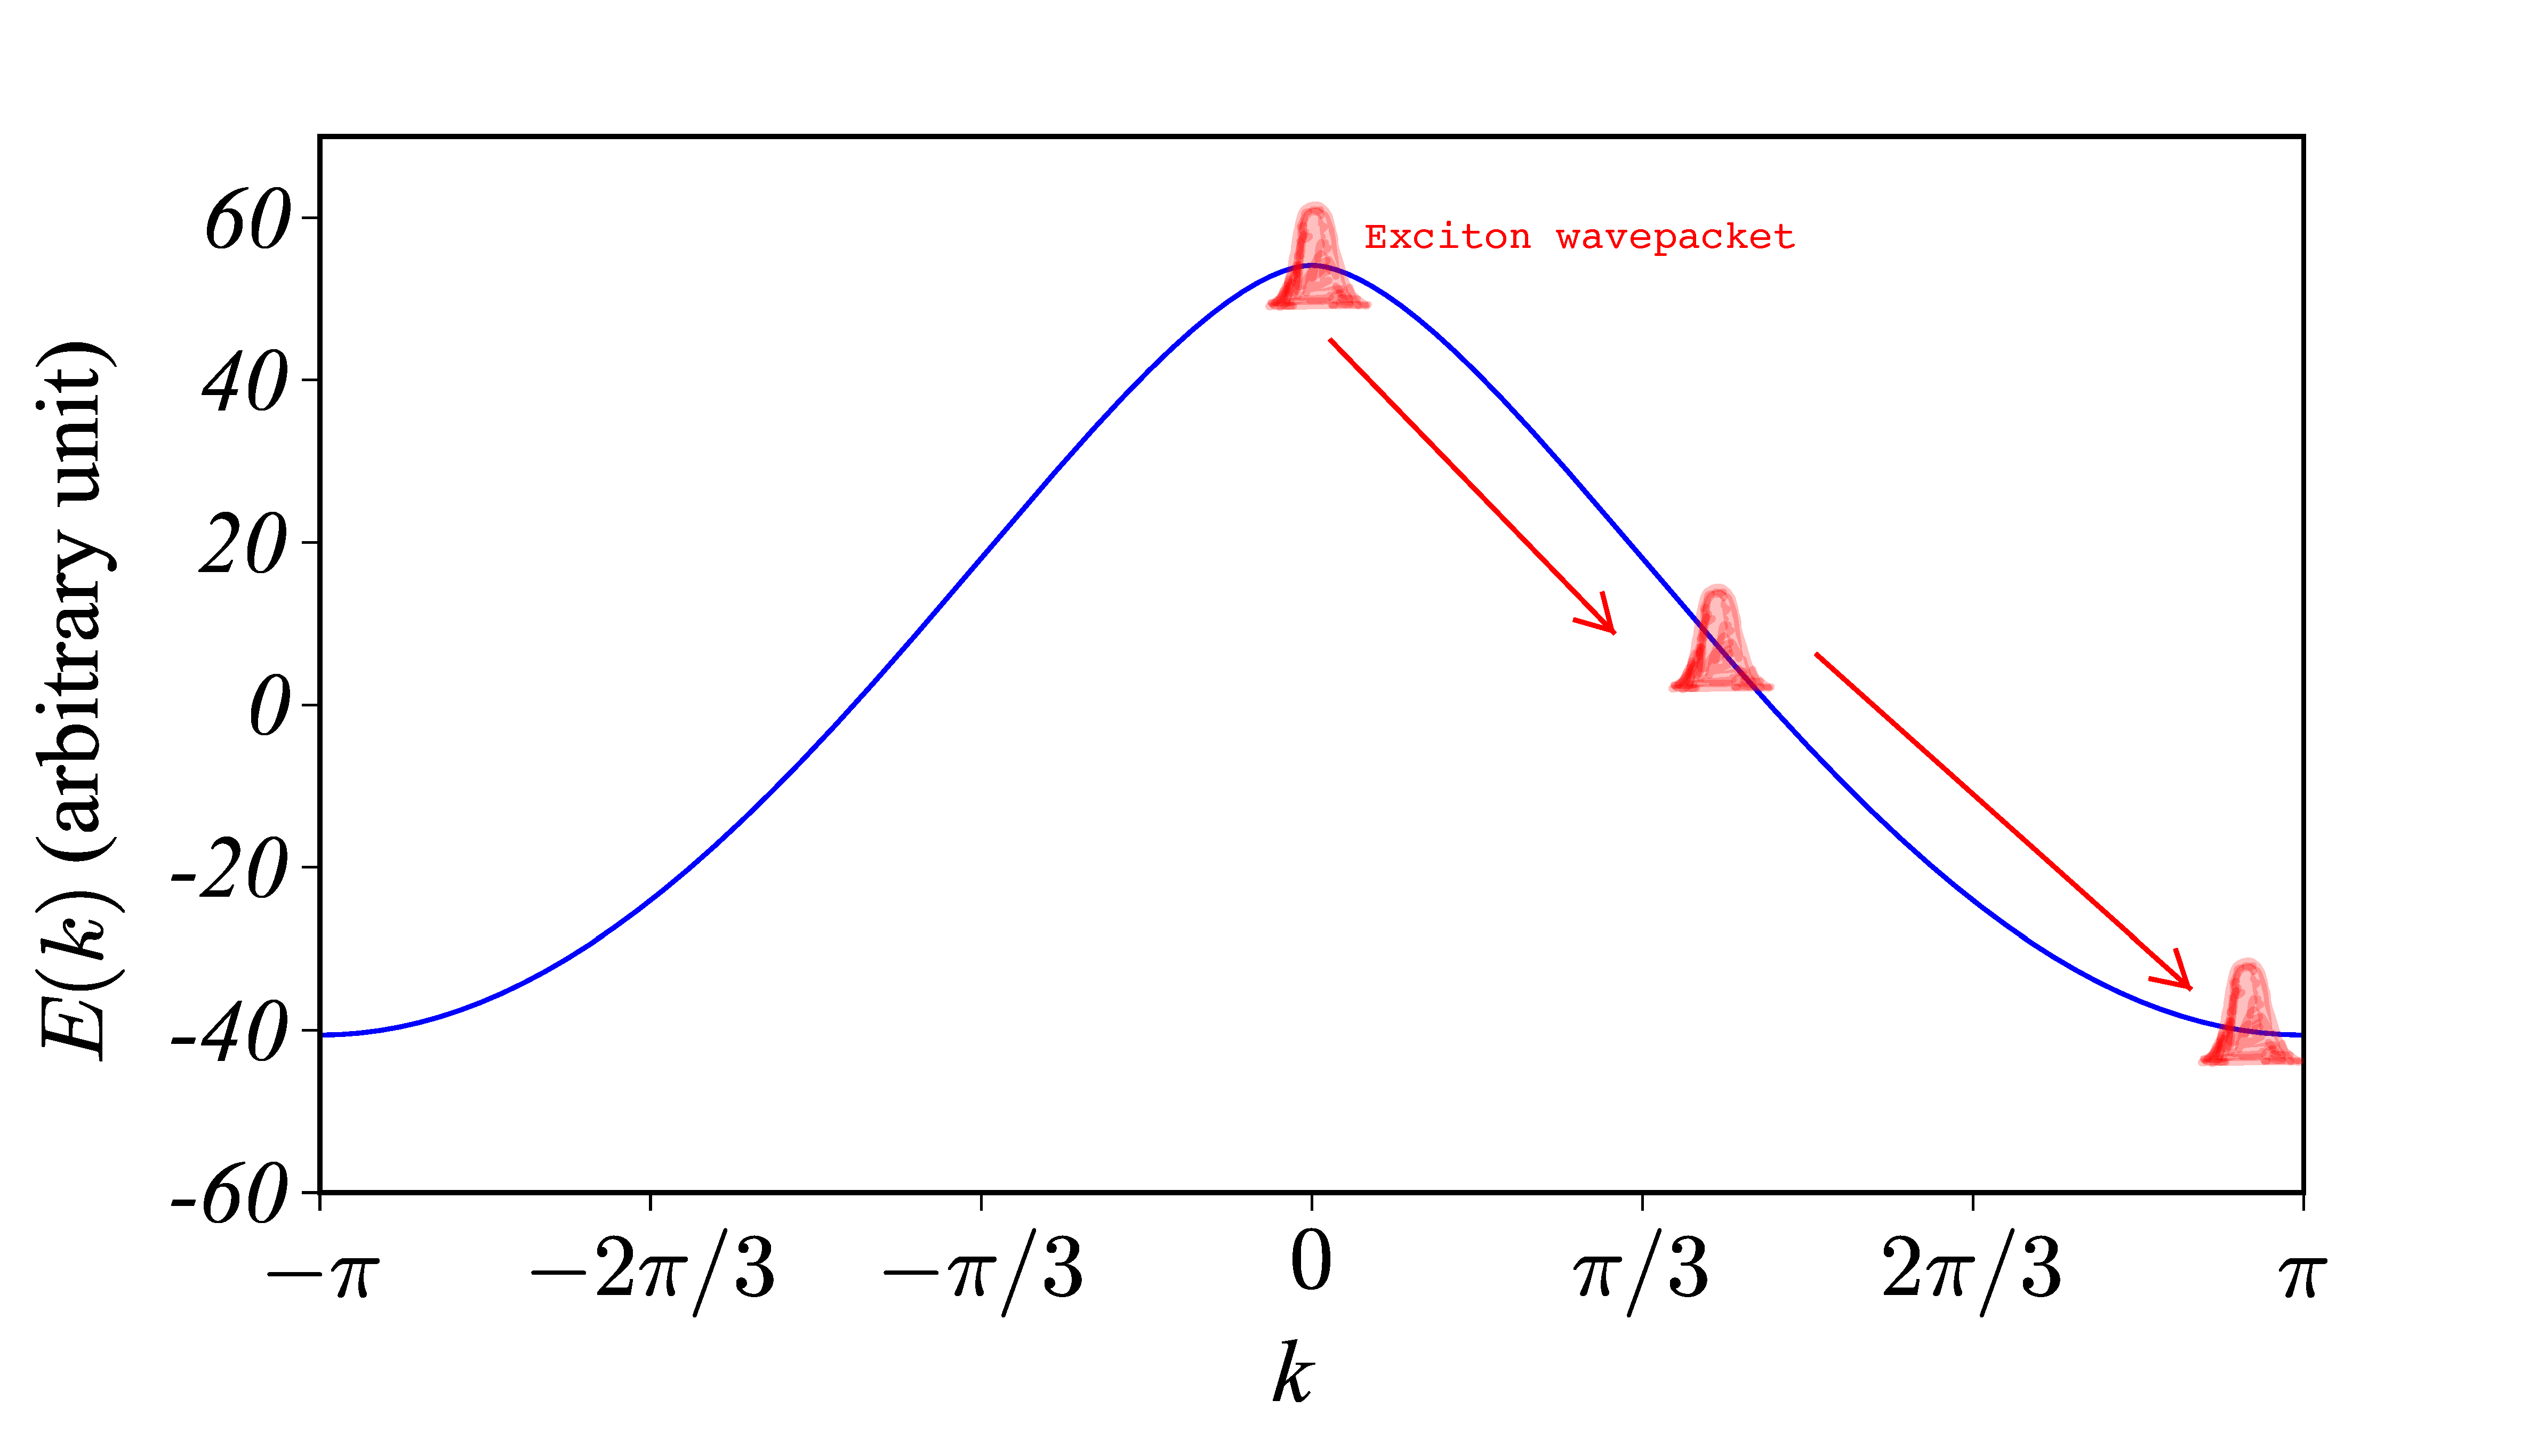
\includegraphics[width=\linewidth]{dispersion-curve-move-wavepacket.png}
\caption{
The dispersion curve of an exciton. The interaction between site $m$ and site $n$ is proportional to $1/|n-m|^3$. 
}
\label{fig:movewave packet}
}


But how do we move an exciton wave packet in $k$ space without changing its shape? We can get some hint from the
expression of the plane wave state
\oneline{
\ket{k(t)} = \frac{1}{\sqrt{N}}\sum_n e^{i k a n} \ket{n(t)} \ . \label{eqn:kStateExpansion}
}
\Autoref{eqn:kStateExpansion} suggests that we can change $\ket{k}$ to $\ket{k+\delta}$ by adding a
 factor $e^{i \delta a n}$ to each term in the expansion.  Since the increment $\delta$ is independent of the $\ket{k}$
state, 
%For modifying the group velocity of a collective excitation, the
%essential idea is to add a factor $e^{i \delta a n}$ to each term
%in the expansion (\ref{basis}), so that 
each $| k\rangle$ component in a wave packet (\autoref{basis}) can be transformed into $|
k+\delta\rangle$ in this way. This transformation shifts the
wave packets by $\delta$ in $k$-space while preserving their
shape. As a result, one can engineer wave packets probing any part
of the dispersion $E(k)$ leading to different group velocity and
shape evolution. 
%The feasibility of such transformation in an ensemble of atoms or molecules on an optical lattice is discussed below and in \autoref{sec:excitationAtomMolecule}. 

Knowing that adding the proper phases is a key step, we now study how to add those phases. There are two
 different time scales involved: one is related to the evolution of the free monomer states, 
$T_m = \hbar/\Delta E_{e-g}$, and the other is related to the excitation population transfer between monomers,
 $T_e = \hbar/\alpha$. Usually, $T_m$ is smaller than $T_e$ by several orders of magnitude. This huge
 difference in magnitude enable us to work with the adiabatic and sudden time scales at the same time as described below. 
%Adding a site-dependent phase to the excitonic wavefunction
%exploits an interplay of the adiabatic and sudden time scales.
Consider  the $n$-th monomer subjected to an external field
$\mathcal{E}_n(t)$ which varies from 0 to some value and then back
to 0 in time $T$. If the variation is adiabatic with respect to
the evolution of the free monomer states, $T\gg T_m$, each eigenstate $|f\rangle$ of the monomer acquires a
state-dependent phase shift \cite{adiabatic-theo}
%
\begin{eqnarray}
\ket{f_n (T)} = e^{i \phi_{n}^f}\ket{f_n(0)},
\label{adiabatic-theorem} \label{phase}
\end{eqnarray}
%
where 
\oneline{
\phi_{n}^f = -\frac{1}{\hbar}\int_{0}^{T} E_{n}^f(t )dt \ , \label{eqn:expressionOfPhase}
}
$E_{n}^f (t)$ is the instantaneous eigenenergy and $f$ can be $e$
or $g$.
%The operator $\hat{P}_n^\dag = |e_n\rangle\langle g_n |$ acquires the phase $\Phi_n = \phi_{n}^e-\phi_{n}^g$.
Now consider the action of such phase change on the collective
excitation state (\ref{basis}). If $T\ll T_e$, the
change is sudden with respect to the excitation transfer between
monomers, so during the time $T$ the excitation probability doesn't have enough time to propagate 
between different monomers and $C_n$'s in \autoref{basis} remain almost the same. Since $G_k$'s are just fourier
transforms of $C_n$'s, $G_k$ will remain the same as well, conserving the shape of the wave packet $|\psi_{\rm exc}\rangle$ in $k$ space. 
 Then the wave packet $|\psi_{\rm exc}\rangle$ acquires a site-dependent
phase $\Phi_n = \phi_{n}^e-\phi_{n}^g$ that will influence each $\ket{k}$ component in the same way. 
If $\Phi_n = \Phi_0 + n a\delta $, then the momentum $\delta$ is imparted onto the
excitonic wavefunction without changing its shape. By analogy with ``pulsed alignment of
molecules'' \cite{alignment-review}, we call this transformation a
``phase kick'' or ``momentum kick''. Its action is also similar to
that of a thin prism on a wavefront of a monochromatic laser beam.

%%%%%%%%%%%%%%%%%%%%%%%%%%%%%%%%%%%%%%%%%%%%%%%%%%%%%%%%%%%%%%%%%%%%%%%%%%%%%%%%
\begin{figure}[htbp]
\centering
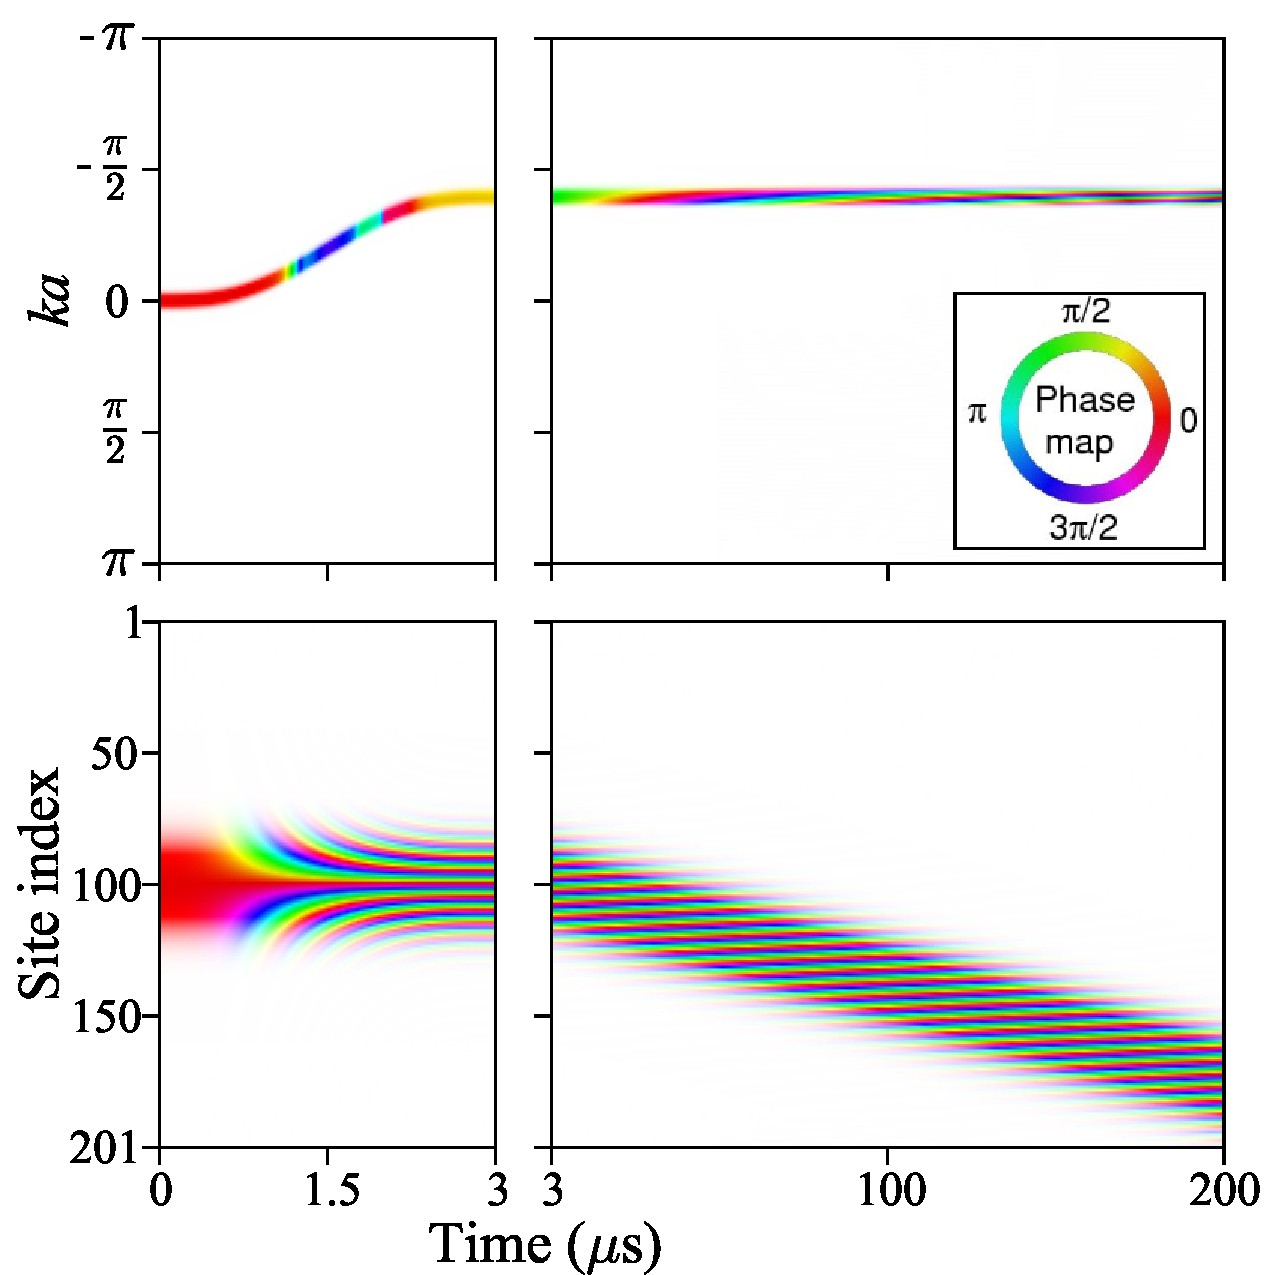
\includegraphics[width=\linewidth]{momentum-kick.pdf}
\caption{
Example of controlled energy transfer in a one-dimensional array of quantum 
monomers subjected to a linear phase transformation. The graph illustrates the evolution of the exciton wave packet  
 centered at $k=0$ and initially positioned at the center of the array. The phase of the wave function
is shown by color.  The brightness of color corresponds to the amplitude of the excitation with white color
 corresponding to zero amplitude. The calculation is for a one-dimensional array
of 201 monomers with $\alpha = 22.83$ kHz and $\Delta E_{e-g} =12.14$ GHz,  and the linear phase transformation 
$\Phi_n \simeq \Phi_0  -1.29 n$. The corresponding experimental setup is illustrated in
 \autoref{fig:experimentalSetup}
%These parameters correspond to LiCs molecules trapped on an optical lattice with lattice constant $a = 400$ nm and
% subjected to a homogeneous DC field of 1 kV/cm directed perpendicular to the
%intermolecular axis. The kicking potential leading to this particular  phase transformation  can be provided by a
%$\lambda = 1064$ nm Gaussian laser beam, with the propagation direction along the array axis, focused to 5 $\mu$m, 
%with the intensity at the focus equal to $10^7$ W/cm$^2$. The laser pulse is on between 0 and  $3 \mu$s.
}
\label{momentum-kick}
\end{figure}
%%%%%%%%%%%%%%%%%%%%%%%%%%%%%%%%%%%%%%%%%%%%%%%%%%%%%%%%%%%%%%%%%%%%%%%%%



In order to illustrate the shifting of exciton wave packets in the
momentum space, we solve numerically the time-dependent
Schr\"{o}dinger equation with the unperturbed Hamiltonian
(\ref{ham}),  subjected to a transient site-dependent external
perturbation that temporarily modulates $\Delta E_{e-g}$.
We choose the parameters $\Delta E_{e-g} =12.14\mbox{ GHz}$, $\alpha =22.83\mbox{ kHz}$ and the lattice constant $a=400\mbox{ nm}$ that correspond to an array of
polar molecules trapped in an optical lattice, as described in detail in \autoref{sec:excitationAtomMolecule}.
The time-dependent perturbation has the form of a short pulse with the duration $T = 3\; \mu s$. %$\tb{T} \approx \frac{1}{15} \hbar/\alpha$.
The phase acquired by the particles during this time is given by $\Phi_n \simeq \Phi_0  -1.29 n $, which can be achieved with a focused laser beam, as described in \autoref{sec:excitationAtomMolecule}.



The excitation at $t=0$ is described by
a Gaussian wave packet of the exciton states $|\psi_{\rm
exc}(k)\rangle$, with the central wavevector $k=0$.
\Autoref{momentum-kick} shows that the
entire wave packet acquires momentum during the external perturbation pulse (left
panels). This is manifested as a phase variation in the coordinate
representation, and as a shift of the central momentum in the
$k$-representation. After the external perturbation is gone, the
wave packet does not evolve in the $k$-representation and moves
with the acquired uniform velocity in the coordinate
representation.

%% add the block oscillation part %%%%%%%%%%%%%%%%%%%
As a side note, we find that if the laser intensity remains the
same after reaching the maximum, the oscillation
of the wave packet in momentum and coordinate space can be observed  (see 
\autoref{bloch-osci}). This phenomenon is a special Bloch oscillation
since the force is acting on a quasi-particle rather than real
particles in conventional cases  \cite{b-oscillation}, which allows for the possibility to study condensed-matter excitations and energy transport without statistical averaging.


%%%%%%%%%%%%%%%%%%%%%%%%%%%%%%%%%%%%%%%%%%%%%
\begin{figure}[htbp]
\centering
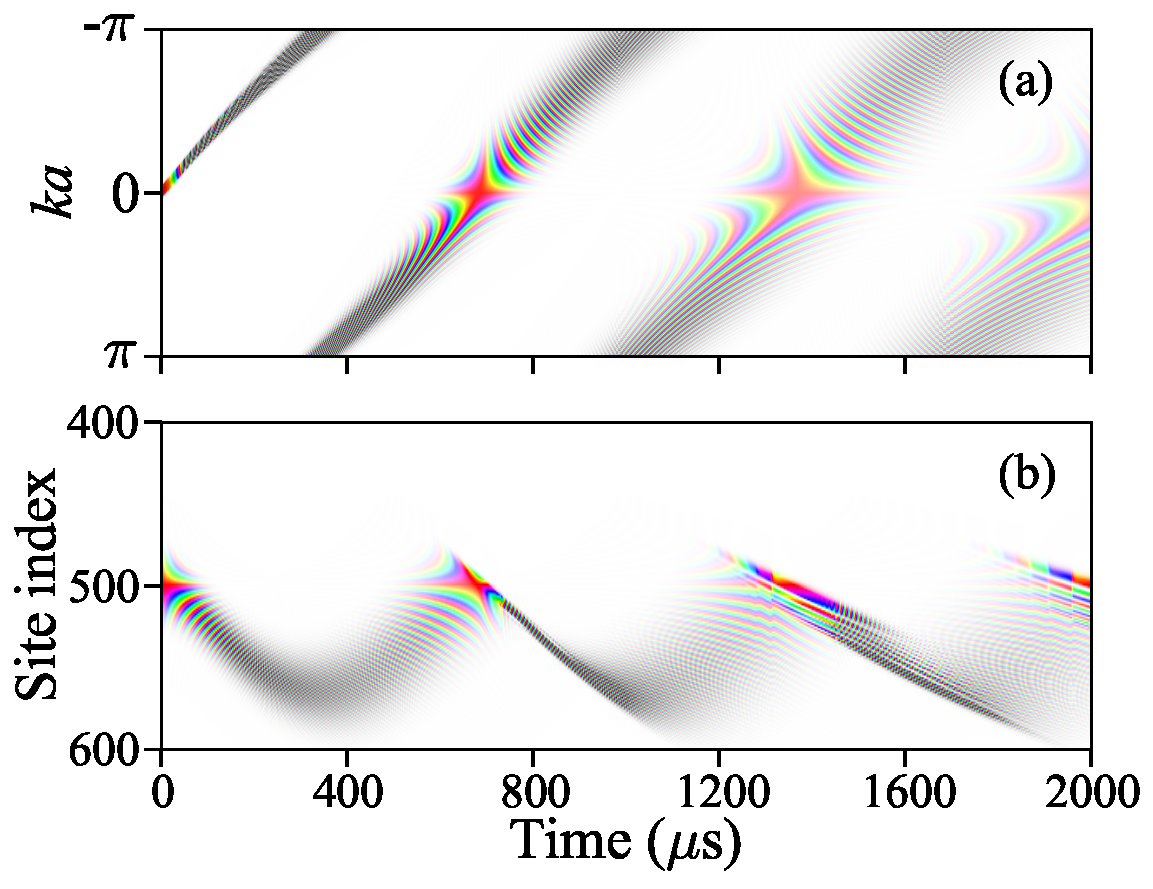
\includegraphics[width=\linewidth]{bloch-osci.pdf}
\caption{``Bloch oscillation" of the exciton wave
packet in the momentum and coordinate spaces. The phase of the
wave function is shown by color as in  \autoref{momentum-kick}. A low laser intensity of $10^6$
W/cm$^2$ is used and all other parameters are the same as in
\autoref{momentum-kick}. Part (a) shows that the wave packet moves in $k$ space
in response to the linear laser field. However, since the wave vector is limited in the first Brillouin zone,
when the wave packet reaches $-\pi$ or $\pi$, it disappears at the boundary and reappears at the other 
boundary. Part (b) presents the motion of the wave packet in coordinate space in accordance with the phase
kicking in $k$ space. Note that the wave packet  spreads in both the momentum and coordinate spaces
because the laser intensity profile along the molecular array is not perfect and this is amplified over extended
time period. 
} 
\label{bloch-osci}
\end{figure}
%%%%%%%%%%%%%%%%%%%%%%%%%%%%%%%%%%%%%%%%%%%%

The results presented in \autoref{momentum-kick}  and all subsequent results of this work are for a single 
collective excitaion in an interacting many-particle system. A general experimental implementation may result in 
multiple excitations, leading to non-linear exciton interactions. There are two mechanisms for exciton - exciton 
interactions: kinematic interactions arising from the statistical properties of excitons and dynamical 
interactions determined by the matrix elements of the inter-particle interactions in the Hilbert sub-space of binary 
excitations \cite{agranovich, marina-bookchapter}. The effects of the kinematic interactions on energy transfer
 in molecular crystals have never been observed so these interactions are considered to be weak, especially in the
 limit of a small number of excitations easily achievable in experiments \cite{kinematic-biexciton-agranovich}. For molecules 
on an optical lattice, the dynamical interactions are important in the presence of strong external electric fields where
 molecular states of different parity are strongly mixed \cite{biexcitons, felipe}.
At weak parity-mixing fields considered here, the exciton-exciton interactions insignificantly mix different $k$ states
 of the individual excitons, contributing weakly  to localization. These effects are expected to be much smaller than
 the disorder-induced perturbations,  discussed in \autoref{sec:energyTransferVacancy}  and \autoref{sec:focusingStrongDisorder}.










\section{Focusing of a delocalized excitation}
\label{sec:focusing}

In order to achieve full control over excitation transfer, it is desirable to find a particular phase transformation
that focuses a delocalized many-body excitation onto a small part of the lattice, ideally a single lattice site.
In optics, a thin lens focuses a collimated light beam by shifting
the phase of the wavefront, thus converting a plane wave to a
converging spherical wave. Similarly, a phase kick can serve as a
time domain ``lens'' for collective excitations: an excitation initially
delocalized over a large number of monomers can be focused onto a
small region of the array after some time. By analogy with optics, a concave or convex
symmetric site-dependent phase $\Phi(n)$ applied simultaneously to
all monomers may turn a broad initial distribution $C_n(t=0)$ into
a narrow one.

The dynamics of the excitation state in the lattice is determined by the time dependence
of the coefficients $C_n(t)$ in  \autoref{basis}. In order to find the expression for $C_n(t)$, we expand the amplitudes
 at $t=0$ in a Fourier series
\begin{eqnarray}
C_n(t=0) = \sum_q
\frac{e^{iq a n}}{\sqrt{N}}C(q; t=0)
\end{eqnarray}
and apply the propagator $e^{-iE(q)t/\hbar}$ to each $q$-component with
$E(q)$ representing the exciton energy given by \autoref{dispersion}.
Transforming the amplitudes $C(q)$ back to the site representation then yields
\begin{equation}
C_m(t) = \frac{1}{N} \sum_{n,k} C_n(t=0) e^{i [\Phi(n) +  k a
(m-n) - E(k) t/\hbar ]},
 \label{Cn(t)}
\end{equation}
where $\Phi(n)$ is a
site-dependent phase applied at $t=0$, as described in the previous section.
Note that the phase $\Phi(n)$ does not have to be applied
instantaneously. The phase  $\Phi(n, t)$ can be applied continuously over an
extended time interval as long as the accumulated phase gives the desired outcome  $\int_0^{T}\Phi(n, t)dt = \Phi(n)$.


\subsection{Focusing to a single site}
\label{sec:singleSiteFocusing}
As \autoref{Cn(t)} shows, the focusing efficiency is determined by the phase transformation and
the shape of the dispersion curve $E(k)$. Given the cosine dispersion of excitons (\ref{dispersion}), is it possible to
 focus a delocalized excitation onto a single lattice site?
To answer this question, we assume an initial condition where the excitation is localized to the site $n_0$, that is,
\multiline{
C_n (t=0) = \delta_{n, n_0} \ ,
}
and run a backward-in-time evolution to calculate the coefficients $C_m(t)$ at $t=-\tau$:
using the expansion of an exponent in Bessel functions (Jacobi-Anger expansion, see Ref. \cite{ jacobi-anger})
\begin{eqnarray}
e^{ia\cos x} = \sum_{n} e^{-i(x-\pi/2)n} J_n(a) \ ,
\end{eqnarray}
we obtain
\multiline{
C_m (-\tau) &=&  \frac{1}{N} \sum_{n,k} C_n(t=0) e^{i [k a
(m-n) - E(k) (-\tau)/\hbar ]} \nonumber \\
&=&  \frac{1}{N} \sum_{n,k} C_n(t=0) e^{i [k a (m-n)}\sum_{n'} e^{- i(ka - \pi/2) n'}  J_{n'}(2\alpha \tau/\hbar) \nonumber \\
&=& \frac{1}{N} \sum_{n,k} \delta_{n, n_0} e^{i [k a (m-n)}\sum_{n'} e^{- i(ka - \pi/2) n'}  J_{n'}(2\alpha \tau/\hbar) \nonumber \\
&=&  \frac{1}{N} \sum_{k} e^{i k a (m-n_0 )}\sum_{n'} e^{- i(ka - \pi/2) n'}  J_{n'}(2\alpha \tau/\hbar) \nonumber \\
&=& \sum_{n'} e^{i\pi n'}  J_{n'}(2\alpha \tau/\hbar) \left( \frac{1}{N}\sum_{k} e^{i k a (m-n_0 - n')}\right) \nonumber \\
&=& \sum_{n'} e^{i\pi n'}  J_{n'}(2\alpha \tau/\hbar) \delta_{n', m-n_0} \nonumber \\
&=& e^{i \pi (m - n_0)/2}J_{m-n_0}\left(2\alpha \tau/\hbar\right) \ , \label{eqn:cosineFocusing}
}
where $J$ is the Bessel function of first kind. 
This  calculation shows that an wavepacket with  the site representation, i.e., 
$C_m(0)= e^{i \pi (m - n_0)/2}J_{m-n_0}\left(2\alpha t/\hbar\right)$,  will focus onto the lattice 
site $n_0$ after evolving for time $t$. We can be easily verify the result by running a forward-in-time evolution
starting with the initial wave packet and making use of 
the orthonormality  of the Bessel functions
\begin{eqnarray}
\sum_{n} J_n(x) J_{n-m}(x) = \delta_{m,0} \ .
\end{eqnarray}
\Autoref{eqn:cosineFocusing} shows that  the focusing of a wave packet onto a
 single site would require not only adding the phase $\Phi(n) = {\rm Arg}[C_m(-\tau)]$, but also the amplitude
 modulations of the coefficients equal to the absolute values of $C_m(-\tau)$. This second task is
 beyond the manipulation tools considered here. However, creating such a wave packet may require multiple and 
complicated phase transformations, which may be difficult to realize in experiments. 


\subsection{Focusing a broad wavepacket in coordinate space}
\label{sec:wavepacketFocusing}

A simpler procedure can be implemented if the phase transformations are restricted to a particular part of
the exciton dispersion.
From wave optics, waves with quadratic dispersion can be
focused, while those with linear dispersion propagate without changing
the wave packet shape \cite{focusing-books-1,focusing-books-2}. It is this interplay of the quadratic (at low $k$) and
 linear (at $k \approx \pm \pi/2a$) parts of the cosine-like exciton dispersion (\autoref{dispersion}) that precludes perfect  focusing of a general collective excitation.
In order to avoid the undesirable amplitude modulations, it may be possible to focus delocalized excitations by a phase transformation that
 constrains the wave packet (\ref{k-rep}) to the quadratic part of the dispersion $E(k)$.  For such wave packets, adding a quadratic phase
$\vp(n) = \vp_{0} (n-n_0)^2$ must lead to
focusing around site $n_0$. Below we illustrate the effect of the quadratic phase transformation for a broad wave packet in coordinate space. In the next subsection (\autoref{sec:planewaveFocusing}), we continue to explore the case of a plane wave. 



Consider a Gaussian wave packet with a narrow width $\sigma_{k, 0}$ which centers around $k=0$ in $k$ space
\multiline{
C_k =  A e^{-\frac{ a^2 k^2}{2\sigma ^2_{k, 0} } } \ , \label{eqn:initialWavepacketInk}
}
where $A$ is some normalization factor. Since these normalization factors doesn't matter for the discussion
 here, we will just ignore them in the following derivations. The wave packet represented by
 \autoref{eqn:initialWavepacketInk} is also a Gaussian wave packet in coordinate space. This can be verified
by the following transformation from $k$ space to coordinate space :
\multiline{
C_n &=&\frac{1}{\sqrt{N}} \sum_{k} C_k(t=0) e^{  i k a n} \nonumber \\
&\approx& \frac{A}{\sqrt{N}} \int_{-\infty}^{\infty} dk \; e^{-\frac{a^2 k^2}{2\sigma ^2_{k, 0} }  + i k a n}  \nonumber \\
&=& \frac{A}{\sqrt{N}} e^{-\frac{n^2 }{2\sigma ^2_{k, 0} } }\int_{-\infty}^{\infty} dk \;  e^{-\frac{1}{2\sigma ^2_{k, 0} } (k a - i  n \sigma^2 )^2 } \nonumber \\
&=& \frac{A}{\sqrt{N}} \frac{\sigma_{k, 0} \sqrt{2\pi} }{a} \; e^{-\frac{n^2 \sigma ^2_{k, 0} }{2 } } \nonumber \\
&\propto&  e^{-\frac{n^2 }{2(1/\sigma_{k, 0} ) ^2} } \ , \label{eqn:initialWavepacketInRealSpace}
} 
where in the second step we use the integration to approximate the summation of $k$ in the first Brillouin zone and 
extend the integration range from $(-\pi/a, \pi/a]$ to $(-\infty, \infty)$ since the width $\sigma_k$ is very small. 
\Autoref{eqn:initialWavepacketInRealSpace} also shows the width of the wave packet in coordinate space is the 
inverse of its width in $k$ space, that is, $\sigma_{x, 0} = 1/\sigma_{k, 0}$. 

To focus the wave packet, we apply an inhomogeneous phase $\Phi(n) = \Phi_0 (n-n_0)^2$ at $t=0$.  Then the wave 
packet becomes
\multiline{
C_n(t=0) \propto e^{-\frac{n^2 }{2(1/\sigma_{k, 0} ) ^2} } \; e^{i \Phi_0 (n-n_0)^2}\ ,
}
which upon a transformation from coordinate space to $k$ space gives rise to
\multiline{
C_k(t=0) &=& \frac{1}{\sqrt{N}}  \sum_{n} C_n(t=0) e^{-i k a n} \nonumber \\
&\approx& \frac{1}{\sqrt{N}} \int_{\infty}^{\infty} dn\; C_n(t=0) e^{-i k a n} \nonumber \\
&\propto& e^{\frac{-a^2 k^2+4 a k n_0 \Phi_0 +2 i n_0^2 \sigma_{k, 0}^2 \Phi_0 }{2 \left(\sigma_{k, 0}^2-2 i \Phi_0 \right)}} \ . \label{eqn:wavepacketInKAfterPhase}
}
The power of $e$ in \autoref{eqn:wavepacketInKAfterPhase} can be separated into a real part and an imaginary part.
Since the imaginary part contributes only a trivial phase to the wavefunction and doesn't change the shape of the 
wave packet, we can ignore it and obtain
\multiline{
C_k(t=0) \propto e^{-\frac{\sigma_{k, 0}^2 (k a - 2 n_0 \Phi_0 )^2 }{2 (\sigma_{k, 0}^4 + 4 \Phi_0^2 )}} \ . \label{eqn:wavepacketInKAfterPhase2}
}
So the width of the wave packet after adding the phase is
\multiline{
\sigma_k(t=0) = \sqrt{ \sigma_{k, 0}^2 + \frac{4 \Phi_0^2 } { \sigma_{k, 0}^2} } \ ,
}
which is obviously larger than the initial width  $\sigma_{k, 0}$. This indicates that the phase applied for focusing
cannot be too large otherwise the wave packet will be broadened beyond the quadratic region of the dispersion
 curve where the focusing scheme doesn't work. Note that the phase does not affect the width of the wave packet 
 in coordinate space since it only adds some phase to the coefficients $C_n(t=0)$ in
 \autoref{eqn:initialWavepacketInRealSpace}. 

To see how the wave packet evolves after the phase adding, we can apply the propagator $e^{-i E(k) t/\hbar}$ to 
\autoref{eqn:wavepacketInKAfterPhase2} and convert the wavefunction into coordinate space. Assuming the width
 $\sigma_k(t=0)$ is very small so that a large proportion of the wave packet is within the quadratic region of the
 dispersion curve, then the eigen energy of of the $\ket{k}$ state can be approximated as
\oneline{
E(k) \approx E_0 + \beta a^2 k^2 \ .  \label{eqn:quadraticApprox}
}
Using \autoref{eqn:quadraticApprox},
we obtain the wavefunction of the wave packet after time $t$
\multiline{
C_n(t) &=& \frac{1}{\sqrt{N} }\sum_{k} e^{ i k a n} e^{-i E(k) t} C_k(0) \nonumber \\
&\propto& \sum_{k} e^{ i k a n} e^{-i E(k) t/\hbar} e^{-\frac{\sigma_{k, 0}^2 (k a - 2 n_0 \Phi_0 )^2 }{2 (\sigma_{k, 0}^4 + 4 \Phi_0^2 )}} \nonumber \\
&\propto& e^{- \frac{(n + 4 t \beta\Phi_0  n_0)^2 }{2 \sigma_{x}(t)^2 } }
}
where $\sigma_{x}(t)$ is a time-dependent width given by
\oneline{
\sigma_{x}(t) = \sigma_{x, 0} \sqrt{ (1 + 4 t \beta \Phi_0 )^2 +  \frac{4 t^2 \beta^2}{\sigma_{x, 0}^4 }} \ .
}
Taking the derivative of $\sigma_{x}(t)$ with respect to time and setting it to zero, we can find the time at which the
wave packet is most focused:
\multiline{
T_{\rm F} = -\frac{\Phi_0  \sigma _{x, 0}^4}{\beta  \left(1+4 \Phi_0 ^2 \sigma _{x, 0}^4\right)} \ .
}
At time $T_{\rm F}$, the minimum width is
\oneline{
\sigma_{x, {\rm F}} = \frac{\sigma _{x, 0} }{\sqrt{ 1+4 \Phi_0 ^2 \sigma _{x, 0}^4 } } \ , \label{eqn:widthAtFocus}
}
and the center of the wave packet is 
\oneline{
n_{\rm c} = 4 T_{\rm F} \beta \Phi_0 n_0 =  \frac{4 \Phi_0 ^2}{\sigma_{k, 0} ^4+4 \Phi_0 ^2} n_0\approx n_0 \ .
}
\Autoref{eqn:widthAtFocus} shows that the wave packet will become more focused at site $n_0$ at $T_{\rm F}$ since $\sigma_{x, {\rm F}} < \sigma _{x, 0} $ and a larger phase $\Phi_0$ will leads to a better focusing effect. However, as we have
discussed before, large values of $\Phi_0$ may take the wave packet outside the quadratic part of the dispersion
 making \autoref{eqn:quadraticApprox} invalid. Therefore, the best focusing effect can only be achieved by balancing
the two influences. 
%First, consider a broad Gaussian wave packet (\ref{basis}) with
%\oneline{
%C_n(\tilde\sigma_x;t=0) =\sqrt{{a}/{\tilde\sigma_x \sqrt{\pi}} }
% \exp \left[- {a^2 (n-n_0)^{2}} / {2\tilde\sigma_{x}^2 } \right]
%}
%where $\tilde\sigma_x \gg a$ {is the initial width. The corresponding width
%in the wave vector space is given by $\sigma_k = 1/\tilde\sigma_x$.
%The application of an inhomogeneous phase $\Phi(n) = \vp_0
%(n-n_0)^2$ at $t=0$ results in additional broadening of the
%initial state, and the total width of the wave packet in the
%wave vector space with the account of the phase-induced contribution
%becomes}
%\cite{focusing-books-1,focusing-books-2} %By applying the quadratic phase to the
%Gaussian wave packet with quadratic dispersion, we have changed
%the original wave packet and the new width in momentum space
%\cite{focusing-books-1,focusing-books-2} becomes
%
%\begin{equation}
%\sigma_{k}(\tilde\sigma_x, \Phi_0)  =
%\frac{1}{\tilde\sigma_x}\,{\sqrt{1 + 4 \Phi_0^2 \tilde\sigma_x^4 /
%a^4 }}. \label{sigma-k}
%\end{equation}
%
%Then we can leave the wave packet to propagate by itself, and
%after some time it will become focused. Since the free propagation
%in the coordinate space doesn't change the width of the wave
%packet in the momentum space, $\sigma_{k}$ will remains the same
%after the phase kicking. Intuitively speaking, for a specific
%$\sigma_{k}$ the best possible focusing can be achieved when
%$\sigma_{k}\sigma_{x}=1$ in accordance with the uncertainty
%principle. Therefore, one would expect to see better focusing when
%large values of $\Phi_0$ produces larger $\sigma_{k}$ according to
%Eq. (\ref{sigma-k}).
%By analogy with optics, one should expect better focusing
%with larger $\Phi_0$ (the width of the wave packet in real space
%is $\sigma_x(\Phi_0) = 1/\sigma_k(\tilde\sigma_x,\Phi_0))$.
%However, large values of $\Phi_0$ may take the wave packet outside the quadratic
%part of the dispersion, impeding the focusing.

In the case of exciton with the cosine dispersion curve represented by \autoref{dispersion}, $\beta = -\alpha a^2$. 
To find the optimal phase $\Phi_0^*$ that keeps the wave packet
within the quadratic dispersion while focusing it, we use the
condition $\sigma_{k, 0} \lesssim 1$, which yields
$\Phi_0^* = \pm 1/2 \sigma_{x, 0}$ for the optimal focusing. At
time
\begin{equation}
t_* \approx 1 / 4 \alpha \Phi_0^* \ , \label{focus-time}
\end{equation}
the wave packet is most
focused and has a width
%
\begin{equation}
a\sigma_{x,F} (\Phi_0^*) =  \frac{ a \sigma_{x, 0}} {\sqrt{1 + 4
\Phi_0^{*\,2} \sigma_{x, 0}^4  }} \sim a .
\label{x-focusing-Gauss}
\end{equation}
For the time $t_*$ in \autoref{focus-time} to be positive, $\alpha$ and $\Phi_0^*$ must have the same sign.
 Therefore, a convex quadratic phase profile
$\Phi(n)$ with $\Phi_0>0$ must focus collective excitations in a system with
repulsive couplings between particles in different lattice sites ($\alpha>0$), and a concave quadratic phase
profile $\Phi(n)$ with $\Phi_0<0$ must focus excitations in a system with
attractive couplings ($\alpha<0$).

\subsection{Focusing a plane wave in coordinate space}
\label{sec:planewaveFocusing}

Consider a completely delocalized excitation (\ref{basis})
with $C_n(k;t=0) = {e^{iakn}}/{\sqrt{N}}$ describing an eigenstate
of an ideal system of $N$ coupled monomers.
Suppose $E(k)$ in \autoref{Cn(t)}  can be approximated as $E(k) = \D E_{e-g}
-\alpha a^2 k^2$. As we have seen in the derivation of last section, the effect of $E(k)$ on the wave packet is to
add a phase due to time evolution, i.e. $e^{-i E(k) t}$. Since $\D E_{e-g}$ in $E(k)$ contributes the same phase to all
$k$ component and thus adds a trivial phase to the whole wavefunction, we can saftely ignore it if only the shape of
the wavefunction is concerned. Therefore, we use   $E(k) = -\alpha a^2 k^2$ instead in the following derivation. To
focus the plane wave, the quadratic phase $\vp(n) = \vp_0
n^2$ are applied at $t=0$. This changes the initial wavefunction to 
\multiline{
C_n(k; t=0) &=&  \frac{1}{\sqrt{N}}  e^{i k a n } e^{i \Phi_0 n^2 } \ ,
}
which renders the wavefunction a wave packet in $k$ space with the coefficient:
\multiline{
C_q(t=0) =\frac{1}{\sqrt{N}} \sum_{n} e^{- i q a n} C_n(k; t=0) \ . \label{eqn:qComponent}
}
Each $q$ component in \autoref{eqn:qComponent} evolves according to 
\multiline{
C_q(t) = e^{-i E(q) t} C_q(0) = e^{i \alpha a^2 q^2} C_q(0) \ ,
}
then the wavefunction in coordinate space after time $t$ is given by
\multiline{
C_m(t) &=& \frac{1}{\sqrt{N}}  \sum_{q} e^{i q a m} C_q(t) \nonumber \\
&=& \frac{1}{N \sqrt{N}}\sum_{q} e^{i q a m} e^{i \alpha a^2 q^2}  \sum_{n} e^{- i q a n} e^{i k a n } e^{i \Phi_0 n^2 } \nonumber \\
&=& \frac{e^{-i\alpha a^2 k^2}}{N}\
\sqrt{\frac{i\pi}{N \Phi_0}} \sum\limits_q e^{i[a^2(k-q)^2 (\alpha
t - 1/4\Phi_0) + q
a (m + 2\alpha ak) ]} \nonumber \\
&&\hspace{0.5cm} \times \Theta\left(-\frac{N\Phi_0}{a} < k-q <
\frac{N\Phi_0}{a}
\right) \ , \label{C_plane_wave}
}
%\begin{equation}
%\begin{array}{c}
%\displaystyle C_m(t) = \frac{e^{-i\alpha a^2 k^2}}{N}\
%\sqrt{\frac{i\pi}{N \Phi_0}} \sum\limits_q e^{i[a^2(k-q)^2 (\alpha
%t - 1/4\Phi_0) + q
%a (m + 2\alpha ak) ]}\times\\
%
%\\
%
%\displaystyle\times\Theta\left(-\frac{N\Phi_0}{a} < k-q <
%\frac{N\Phi_0}{a}
%\right),\\
%\end{array}\label{C_plane_wave}
%\end{equation}
where $\Theta(z) = 1$ if $z$ is true and zero otherwise.
In order to derive \autoref{C_plane_wave}, we
used the approximate equality
\begin{equation}\label{approx integral}
\int\limits_{-M}^M dx\ e^{-i(ax^2 + b x)} \approx
\sqrt{\frac{\pi}{ia}}\ e^{i b^2/4a}\  \Theta(-2Ma < b < 2Ma),
\end{equation}
obtained by approximating the error function of a complex argument
${\rm Erf}(\sqrt{i}x)$ by the sign function, which is accurate for
large argument $x$.

At time $t_* = 1/4\alpha\Phi_0$, the terms quadratic in $q$
in \autoref{C_plane_wave} are canceled, and the sum over $q$ reduces to a
delta-function, if the summation limits are from $-\pi/a$ to
$\pi/a$. Therefore, the choice $\Phi_0 = \pi / N$ yields 
\oneline{
C_m(t) =\sqrt{i} e^{-i N a^2 k^2 / 4\pi} \delta_{m,-\nu_k} \ , \label{eqn:cmPlaneWave}
}
where   $\nu_k$
is the index of the initial wave vector $k = 2\pi \nu_k / Na$, quantized due to the discreteness of the lattice.
%However, this works well for a true quadratic dispersion only.
According to step function  $\Theta(z)$ in \autoref{C_plane_wave}, the dimensionless width
of the wave packet in the wave vector space is $\Delta_k(\Phi_0)
\equiv a\sigma_{k}(\Phi_0) \approx 2N\Phi_0$. When $\Phi_0 = \pi /
N$, the wave packet spreads over the entire Brillouin zone, including the
linear parts of the exciton dispersion.
Using \autoref{approx integral} we find that for an arbitrary
value of $\Delta_{k}(\Phi_0)$, the site amplitudes at the time of
focusing $t_* = 1/4\alpha\Phi_0$ are
\begin{equation}
C_n(k; t=t_*) \approx \frac{e^{i\Delta(\Phi_0) n^2/2N}}{n}
\sqrt{\frac{2i}{\pi \Delta_{k}(\Phi_0)}} \sin (n
\Delta_{k}(\Phi_0) /2). \label{x-focusing-PlaneWave}
\end{equation}
%
In order to keep the linear part of the dispersion spectrum
unpopulated, we choose the optimal focusing phase $\Phi_0^*
\sim 1 /2N$, so that $\Delta_{k}( \Phi_0^*)\sim 1$.



\subsection{Numerical results}
\label{sec:focusingNumerical}

In \autoref{sec:wavepacketFocusing} and \autoref{sec:planewaveFocusing}, \autoref{x-focusing-Gauss} and \autoref{x-focusing-PlaneWave} are derived based on the cosine dispersion curve which are
valid for a many-body system with nearest neighbor interactions
only. In most physical systems, the energy dispersion is modified
by long-range couplings. In order to confirm that the above
predictions are also valid for systems with long-range
 interactions and illustrate the focusing of
delocalized excitations, we compute the time evolution of the wave
packets by solving the wave equation numerically for a system with
long-range dipole-dipole interactions. In the calculations, we expanded the Hamiltonian (\ref{ham}) in the site 
basis, i.e. $\{ |e_n\rangle \prod_{i\neq n} |g_i\rangle\}$,  and applied the corresponding phase to the state
$\ket{e_n}$ of each site at $t=0$ and then run the time evolution to obtain the wavefunction at each time point and 
save them to files. To find the time for the optimal focusing, we searched for the largest probability at the target focusing site while scanning the wavefunctions at every time point.  
Figure \ref{focusing-1d}
illustrates the focusing dynamics of a completely delocalized
excitation (panels a and b) and a broad Gaussian wave packet (panels c and d) in a
system with all (first neighbour, second neighbour, etc.) couplings explicitly included  in the
calculation. The results show that  
the collective excitations can be focused to a few lattice sites. The role of the long-range coupling will be
explicitly discussed in \autoref{sec:energyTransferVacancy}. 

%%%%%%%%%%%%%%%%%%%%%%%%%%%%%%%%%%%%%%%%%%%%%%%%%%%%%%%%%%%%%%%%
\begin{figure}[htbp]
\centering
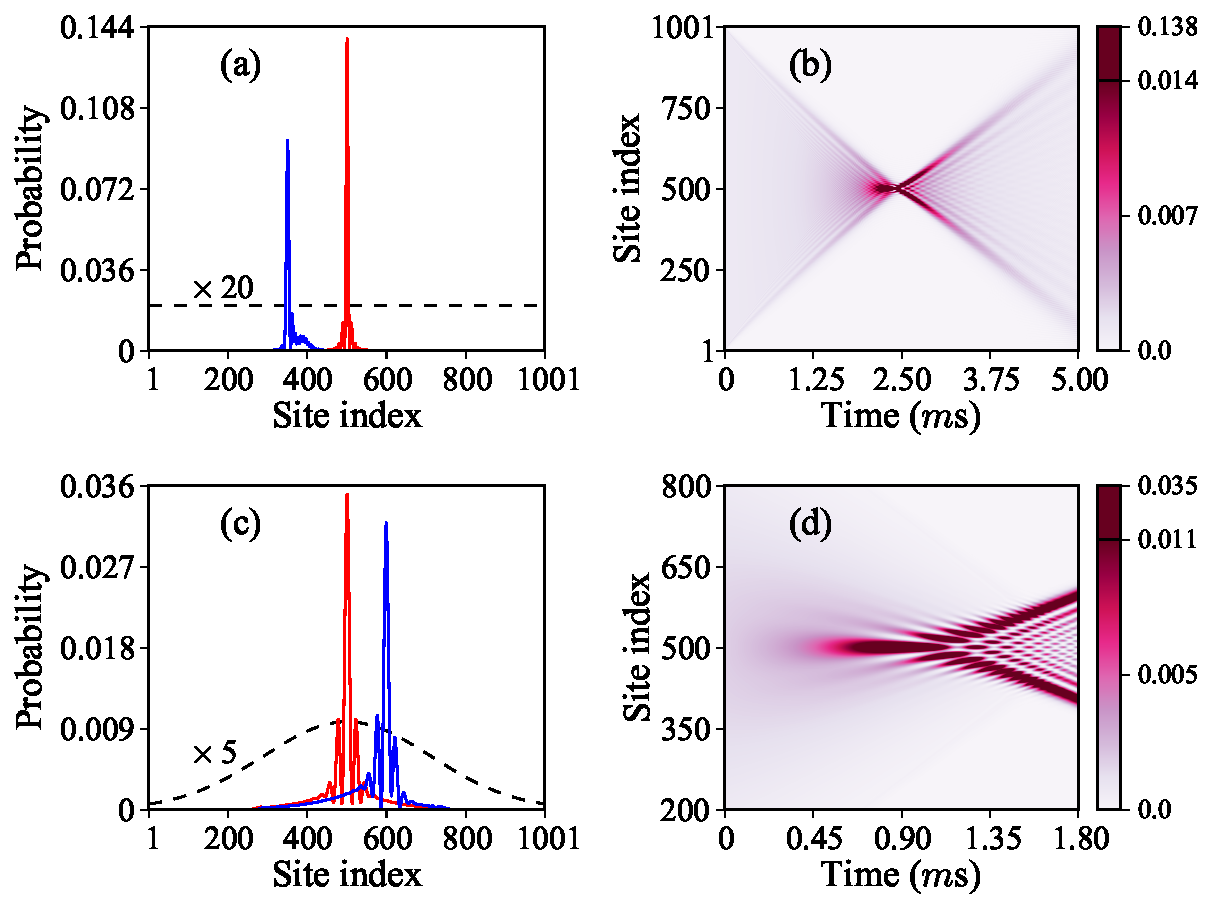
\includegraphics[width=\linewidth]{focusing-1d.pdf}
\caption{ Focusing of a completely delocalized collective
excitation (panels a and b) and a broad Gaussian wave packet of
Frenkel excitons (panels c and d) in a one-dimensional array using the quadratic phase
transformations at $t=0$ as described in text. In panels (b) and (d),
the excitation probability distribution is displayed by color.
The dashed lines
show the initial distribution magnified by 20 and 5 respectively
in (a) and (c). The solid curves in panels (a) and (c) correspond
to two different phase transformations focusing the same wave
packet onto different parts of the array.  The calculations are
performed with the same parameters $\alpha$, $a$, and $\Delta
E_{e-g}$ as in Figure \ref{momentum-kick}. The results are computed
with all couplings accounted for. }\label{focusing-1d}
\end{figure}
%%%%%%%%%%%%%%%%%%%%%%%%%%%%%%%%%%%%%%%%%%%%%%%%%%%%%%%%%%%%%%%%

The focusing scheme demonstrated above can be generalized to  systems of higher
dimensionality. To illustrate this, we repeated the calculations
presented in Figures \ref{focusing-1d} (c) and \ref{focusing-1d} (d) for
a delocalized excitation placed in a square 2D lattice with an external
potential that modulates the phase as a function of both $x$ and
$y$. \Autoref{focusing-2d} shows the focusing of an initially broad wave packet
onto different parts of a 2D lattice induced by the quadratic
phase transformation $\Phi(x,y) = \Phi_0[ (n_x - n_{x_0})^2 + (n_y- n_{y_0})^2]$, 
where $n_x$ and $n_y$ are the lattice site indices along the $x$ and $y$ directions. 
The calculations include all long-range couplings as in \autoref{focusing-1d}. The comparison of \autoref{focusing-1d} and \autoref{focusing-2d} illustrates that the 
focussing efficiency in 2D is greater. The results also demonstrate that the delocalized excitations can be effectively focused on different parts of the lattice simply by varying the reference site $(n_{x_0}, n_{y_0})$ in the phase transformation. 
%Multiple phase kicks of varying profiles separated by periods of free evolution may enable arbitrary shaping of the excitonic wave packet in the coordinate and $k$-spaces.

%%%%%%%%%%%%%%%%%%%%%%%%%%%%%%%%%%%%%%%%%%%%%%%%%%%%%%%%%%%%%%%%%%%%%%%%%%%%%%%%%
\begin{figure}[htbp]
\centering
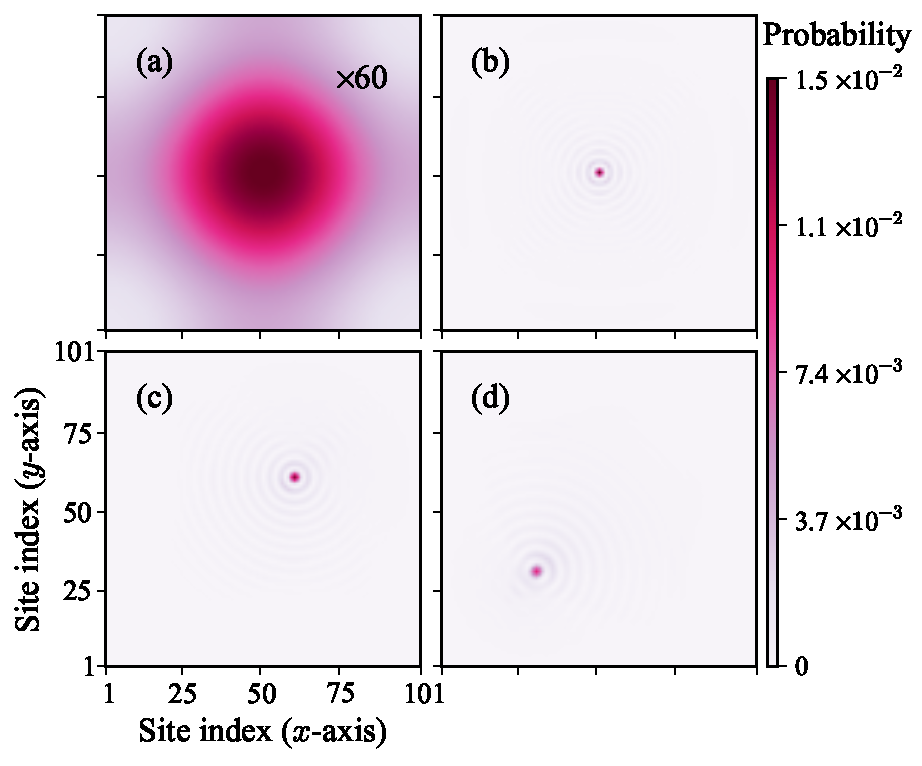
\includegraphics[width=\linewidth]{focusing-2d.pdf}
\caption{Focusing of a delocalized excitation in a 2D array shown
at $t=0$ in panel (a) onto different parts of the lattice (panels
b--d). For better visualization, the probability  distribution in panel (a) is magnified by a factor of 60. The calculations are performed with
the same parameters $\alpha$, $a$, and $\Delta E_{e-g}$ as in
Figure \ref{momentum-kick} and the quadratic phase transformation
at $t=0$.
 }\label{focusing-2d}
\end{figure}
%%%%%%%%%%%%%%%%%%%%%%%%%%%%%%%%%%%%%%%%%%%%%%%%%%%%%%%%%%%%%%%%%%%%%%%%%%%%%%%%%%%


%\section{Controlled excitations of ultracold atoms and molecules}
\section{ Experimental feasibility of phase transformation}
\label{sec:excitationAtomMolecule}

In  \autoref{sec:phaseKicking}  and \autoref{sec:focusing}, we have discussed the idea of phase kicking and its
 application in focusing delocalized excitations, but we were mainly concerned with the theoretical perspective. So in 
this section, we focus on the experimental feasibility and show
the techniques proposed in \autoref{sec:phaseKicking}  and \autoref{sec:focusing}  can be realized with ultracold atoms or molecules trapped in an
optical lattice  with one particle per lattice site \cite{atom-mott1, atom-mott2, atom-mott3, Ye-arrays-PRL12}.
There are three general requirements that must be satisfied:

\begin{itemize}
\item
 (i) The time required for a  phase transformation must
be shorter than the spontaneous decay time of the excited
state.

\item
 (ii) The overall coherence of the system  must be preserved
on the time scale of the excitonic evolution in the entire array, set by $K\hbar/\alpha$, where $K$
 is the number of monomers participating in the dynamics of the collective excitation.

\item
(iii) The lattice constant must be large enough to allow considerable variation of the external
 perturbation from site to site.

%
\end{itemize}

Optical lattices offer long coherence times ($> 1$ sec) and large lattice constants ($>400$ nm)
 \cite{optical-lattice-review}. The lifetime of the
collective excitations depends on the internal states
 of the particles used in the experiment and the momentum distribution of the excitonic states in the wave packet
(\ref{k-rep}). In the following two subsections, we discuss the case of ultracold atoms and the case of ultracold molecules separately. 

%\subsection{Collective excitation of ultracold atoms}
\subsection{Supressing spontaneous emission in system of ultracold atoms}
\label{sec:excitationAtoms}

For ultracold alkali metal atoms in an optical lattice, an optical excitation may generate collective states (\ref{basis}),
as discussed in Ref. \cite{electronic-exciton1, electronic-exciton2}. The lifetime of these excited states is limited by the spontaneous emission of the electronically excited atoms and is
in the range of 10 - 30 ns.
However, the collective excited states can be protected from spontaneous emission if the wave vector range populated by excitons in the wave packet (\ref{k-rep}) is
%sufficiently far from zero \cite{cone-matter-papers}. Due to momentum conservation,
outside of the so-called light cone, so that $k >\Delta E_{e-g}/\hbar c$.  To understand why this is the case, we 
investigate the interaction of the collective excitation state of atoms with light. An photon can excite an exciton
 state of ultracold atoms and the exciton can also decay as a photon. 
During these optical processes,  the energy is conserved, which leads to 
\oneline{
E_{\rm ph} =\hbar c k = \hbar c \sqrt{k_{\parallel}^2 + k_{\perp}^2} = E_{\rm ex}(k_{\rm ex}) \ , \label{eqn:photonExciton}
}
where $k$ and $k_{\rm ex}$ are the wave vectors of the photon and the exciton respectively. As written in
 \autoref{eqn:photonExciton}, the wave vector of the photon can be decomposed into two parts: the part 
($k_{\parallel}$) that is parallel to $k_{\rm ex}$; and the other part ($k_{\perp}$) that is perpendicular to
 $k_{\rm ex}$. Since only the parallel component of $k$ is conserved in the optical excitation, we have
\oneline{
k_{\parallel} = k_{\rm ex} < k \ . \label{eqn:wavevectorConservation}
}
The exciton energy $E_{\rm ex}(k_{\rm ex})$ in \autoref{eqn:photonExciton} can be approximated by the
 corresponding excitation energy $ \Delta E_{e-g}$ since the interaction $\alpha$ between atoms is much smaller
 than the energy gap between the ground state and the excited state of a single atom 
(see \autoref{eqn:dispersionExact}). Then the wave vector of the photon can be calculated from \autoref{eqn:photonExciton}:
\oneline{
k_* = \frac {\Delta E_{e-g}}{ \hbar c} \ .
}
Since the wave vector $k_{\rm ex}$ is just the parallel component of $k_{*}$, only the excitonic states with 
$k_{\rm ex} \leq k_*$  can satisfy both the energy conservation (\autoref{eqn:photonExciton}) and the momentum
 conservation (\autoref{eqn:wavevectorConservation}) at the same time, and thus interact with light. 
%The number of $k$-states in the bright and dark regions depends on the relation between the wavelength of the 
%excitation $\lambda_0 = 2\pi c \hbar / \Delta E_{e-g} $ and the lattice constant, with bright states appearing at $k < k_* = 2\pi / \lambda_0$, and dark
%states at $k_* < k < \pi/a$. 
By comparing $k_*$ and the largest value of $k_{\rm ex}$ in the first Brillouin zone $(-\pi/a, \pi/a]$, we can obtain
the number of excitonic $k$-states in the bright and dark regions. 
For Frenkel excitons originating from electronic transitions in solid-state crystals, the wavelength of excitation light
 $\lambda_0$ ($\sim$ several hundred nm) is much bigger than the lattice constant $a$ ($\sim$ a few {\AA}), the bright region is 
narrow: $ k_{\rm ex} < k_* = 2\pi/\lambda_0\approx 0$. For atoms trapped in optical lattices, the typical values of $\lambda_0$ are of the same magnitude as the lattice constant $a$ (several hundred nm), and a large portion of the
 dispersion curve lies in the bright region and the dark region may be narrow. 
 In an ideal infinite system those states in the dark region have infinitely long radiative lifetimes, as there is no free-space 
photon they can emit, assuming the conservation of both energy and momentum \cite{electronic-exciton1, 
electronic-exciton2, agranovich1966, agranovich}.
In finite and/or disordered systems, the emission of photons may occur at the array boundaries or due to perturbations 
breaking the translational symmetry. In this case, the time scale for spontaneous decay must depend on 
the size of the system (i.e. the probability of the excitation to reach the array boundary) and the disorder potential 
breaking the translational symmetry.  

 %Due to the same conservation laws,
%single-photon excitation of atomic ensembles always generates excitons with $k \approx 0$.
Once collective excited states are created, the phase-kicking technique introduced in  \autoref{sec:phaseKicking}, 
if implemented on a time scale faster than the radiative lifetime of a single atom, 
can be used to shift the excited states in the wave vector space
away from the bright region (cf. \autoref{momentum-kick}) and thus protect the excited states from fast spontaneous decay. This phase transformation can be induced by a pulse of an off-resonant laser field $\mathcal{E}_{AC}$,
detuned from the  $e \leftrightarrow g$ resonance by the value  $\delta\omega$, leading to the
AC Stark shift {(see e.g. Ref.\cite{focusing-books-1})}
\begin{equation}
\Delta E_{AC} =  \mathcal{E}_{AC}^2 \frac{V_{eg}^2}{4 \delta \omega} \ ,
\end{equation}
where $V_{eg}$ is the matrix element of the dipole-induced transition.   By choosing $ V_{eg}= 1$ a.u.,
$\delta \omega = 3 V_{eg}$, and the laser intensity $I = 5\times10^{10}$ W/cm$^2$, we obtain that the shift
 $\phi = \D E_{AC} \times T_{\rm pulse} = \pi $ can be achieved in less than 1 ns. 
%{This shift brings a wave packet initially centered at $k=0$ to the ``dark" edge of the Brillouin zone, where the dispersion of excitons is still quadratic and all the focusing schemes discussed in Section 3 can be applied. 
Another phase transformation can bring the excited state back to the bright region, where it can be observed via fast spontaneous emission. 
 The experiments with ultracold atoms have demonstrated  the lattice filling factor reaching 99 \%  \cite{atom-mott1, atom-mott2, atom-mott3}.
 The phase transformations proposed here can be used to stabilize excitonic states in ultracold atomic ensembles against spontaneous emission  
for multiple interesting applications \cite{Zoubi1, Zoubi-review}. 

%\begin{equation}
%\D E_{AC} = \mathcal{E}_{AC}^2 \frac{V_{eg}^2}{\delta\omega^2},
%\end{equation}
%where $V_{eg}$ is the matrix elements of the dipole-induced transition.
%By choosing $\delta\omega = V_{eg}/5$,
%and the laser intensity $I = 10^{10}$ W/cm$^2$, we obtain that the
%shift $\phi = \D E_{AC} \times T_{\rm pulse} = \pi $ can be achieved
%in less than 10 ns.

%\subsection{Collective excitation of ultracold molecules}
\subsection{Phase kicking in system of ultracold molecules}
\label{sec:phaseKickingMolecules}

The spontaneous decay problem can be completely avoided by using rotational excitations in an ensemble of
ultracold polar molecules trapped in an optical lattice.
The rotational states are labeled by the quantum
number of the rotational angular momentum $\bm{J}$ and the
projection $M_J$ of $\bm{J}$ on the space-fixed quantization axis
$Z$. We choose the rotational ground state $|J=0, M_J=0\rangle$ as
$|g\rangle$ and the rotational excited state $|J=1, M_J = 0
\rangle$ as $|e\rangle$. The state $|J=1, M_J = 0 \rangle$ is
degenerate with the states $|J=1, M_J = \pm 1 \rangle$. This
degeneracy can be lifted by applying a homogeneous DC electric
field, making the $|g\rangle$ and $|e\rangle$ states an isolated
two-level system. The molecules in different lattice sites are
coupled by the dipole-dipole interaction $V_{\rm dd}(n-m)$.
The magnitude of
the coupling constant $\alpha(n-m) = \langle e_{n} , g_{m} |
{V}_{\rm dd}(n-m) | g_{n}, e_{m} \rangle$ between molecules with
the dipole moment $1$ Debye separated by 500 nm is on the order of
1 kHz \cite{felipe}. Due to the low value of $\Delta E_{e-g}$, the spontaneous emission time of
rotationally excited molecules  exceeds 1 second.

%\tz{discuss decoherence - coupling to phonons, and spontaneous emission time}

For molecules on an optical lattice, one can implement the phase
kicks by modifying the molecular energy levels with pulsed AC or
DC electric fields. The rotational energy levels for $^1\Sigma$
molecules in a combination of weak AC and DC electric fields are
given by \cite{friedrich-95}
\begin{eqnarray}
E_{J,M_J}  &\approx&  BJ(J+1) +  \frac{\mu^2 \mathcal{E}_{DC}^2
}{2B} G(J,M_J) \nonumber \\
&& - \frac{ \alpha_{\perp}\mathcal{E}_{AC}^2 }{4} + \frac{
(\alpha_{||}-\alpha_{\perp})\mathcal{E}_{AC}^2 }{4}F(J,M_J)
 \label{DressedEnery-Sum}
\end{eqnarray}
%
where $B$ is the rotational constant,  and $G(J, M_J)$ is given by
\oneline{
G(J, M_J) = \frac{J^2 - | M_J |^2}{J (2 J + 1) (2 J - 1)} - \frac{(J+1)^2 - | M_J |^2}{(J + 1) (2 J + 1) (2 J + 3)} \ ,
}
and $F(J, M_J)$ is given by
\oneline{
F(J, M_J ) = -\frac{1}{2} \left[ 1 - \frac{(2 |M_J | - 1) (2 | M_J | + 1)}{ (2 J - 1) (2 J + 3)} \right] \ ,
}
%$G(0,0) = -1/3$, $G(1,0) =1/5$, $F(0,0) = -1/3$, $F(1,0) = -3/5$, 
and $\mathcal{E}_{AC}$ is the
envelope of the quickly oscillating AC field, $\alpha_\|$ and
$\alpha_{\perp}$ are the parallel and perpendicular
polarizabilities and $\mu$ is the permanent dipole moment of the
molecule.

The momentum shift of the exciton wave packets can be achieved by
applying a time-varying DC electric field $\mathcal{E}(t)
=\mathcal{E}_{\ast} + \mathcal{E}(n)\sin^{2}(\pi t/T)$, where
$\mathcal{E}(n)$ is linear with respect to $n$. Assuming that
$\mathcal{E}(n) = (n-n_0) A$ and $\mathcal{E}(n) \ll
\mathcal{E}_{{\ast}}$, and using \autoref{eqn:expressionOfPhase} and
\autoref{DressedEnery-Sum}, we obtain the phase accumulated by the excited state $\ket{1, 0}_{n}$ at site $n$ with
 respect to the ground state:
\multiline{
\phi(n) &=&  -\frac{1}{\hbar}\int_{0}^{T} \left[ E_{n}^e (t ) - E_{n}^g (t)\right] dt \nonumber \\
&=&  -\frac{1}{\hbar}\int_{0}^{T} \frac{\mu^2 \mathcal{E}_{DC}^2
}{2B}  \left[ G(1,0) - G(0,0)\right] dt \nonumber \\
&=& -\frac{4 \mu^2 }{15\hbar B} \int_{0}^{T}  \left[ \mathcal{E}_{\ast} + A\sin^{2}(\pi t/T) (n - n_0)^2\right] dt \nonumber \\
&\approx& -\frac{4 \mu^2 }{15\hbar B} \int_{0}^{T}  \left[ \mathcal{E}_{\ast}^2 + 2 \mathcal{E}_{\ast} A\sin^{2}(\pi t/T) (n - n_0)\right] dt \nonumber \\
&=&  -\frac{4 \mu^2 }{15\hbar B} \int_{0}^{T}  \left[ \mathcal{E}_{\ast}^2 T +  T \mathcal{E}_{\ast} A (n - n_0) \right] \ . \label{eqn:estimatePhaseDCField}
}
In the above equation, the term that is linear with lattice index $n$ will gives the phase kick
\oneline{
\delta = - 4 A \mathcal{E}_{{\ast}} \mu^2 T / 15 \hbar B a \ .
}
 We have confirmed
this result by a numerical computation showing that for LiCs
molecules in an electric field of $\mathcal{E}_{{\ast}}=1$ kV/cm,
an electric field pulse with $A=7.434\times 10^{-4}$ kV/cm and
$T=1$ $\mu$s results in a kick of $\delta =- \pi/2 a$, bringing an
excitonic wave packet from the $k=0$ region to the middle of the
dispersion zone.

\addfigure{
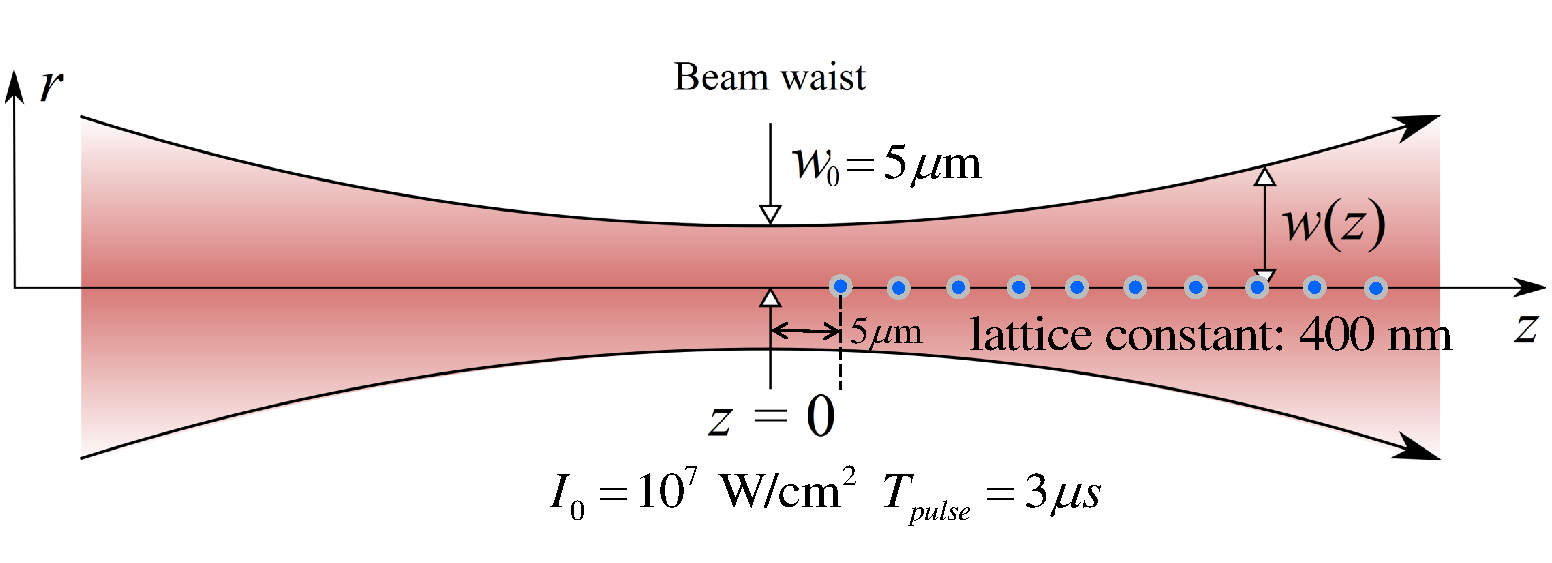
\includegraphics[width=\linewidth]{accelerate-wavepacket-experiment.pdf}
\caption{The experimental setup for the calculation corresponding to \autoref{momentum-kick}. A 1D array of LiCs molecules trapped on an optical lattice with lattice constant $a = 400$ nm is 
 subjected to a homogeneous DC field of 1 kV/cm directed perpendicular to the
intermolecular axis. The kicking potential leading to the  phase transformation  presented by \autoref{Kick-AC} can be provided by a
$\lambda = 1064$ nm Gaussian laser beam that is linearly polarized in the direction of the DC field, with the propagation direction along the array axis, focused to a radius of
 5 $\mu$m, with the intensity at the focus equal to $10^7$ W/cm$^2$. The laser pulse is on between 0 and  $3 \mu$s.
 }
\label{fig:experimentalSetup}
}

An alternative strategy is to use a pulse of an
off-resonance laser field, as for atoms. The phase transformations can be induced
by a Gaussian laser beam with the intensity profile
\begin{equation}
I(r, z) = \frac{I_0}{1+
\frac{z^2}{z_R^2}}\exp\left[-\frac{2r^2}{w_0^2\left (1+
\frac{z^2}{z_R^2}\right) }\right] \ ,
\label{gaussian-intensity-profile}
\end{equation}
where $I_0$ is the light intensity at the beam center, $r$ is the
radial distance from the center axis of the beam, $z$ is the axial
distance from the beam center,  $z_R=\pi w_0^2/\lambda$ is
Rayleigh range, $w_0$ is the beam waist and $\lambda$ is the wavelength.
%% %%%%%%%% recover my old writing %%%%%%%%%%%
In order for the dressed rotational states $\ket{J, M_J}$ have a definite space quantization axis, the laser is linearly polarized in the direction of the DC field. 
As shown in \autoref{fig:experimentalSetup}, we put the 1D molecular array  along the z-axis of
the beam so that $r=0$ for all the molecules. 
Based on Eq.
(\ref{gaussian-intensity-profile}), we can write out the
intensity for each molecule of the array:
\begin{equation}
I(n) = \frac{I_0}{1+ \frac{(z_0 + na)^2}{z_R^2}} \  ,
\label{gaussian-intensity-profile2}
\end{equation}
where $n$ is the molecule index and $z_0$ is the distance between
the center of the wave packet and the beam center.
Suppose the width of
the wave packet in coordinate space is about $S_x$ (positive
integer) times of the lattice constant $a$ and we want to use the
laser gaussian beam to give the wave packet a momentum kick. For
convenience,  the molecule at the center of the wave packet is
indexed as 0, the molecules to the left are indexed by negative
integers and  the molecules to the right by positive integers.  In
practices, we can assume that the wave packet is confined within
the range $[-S_x a, S_x a]$ for a time period much shorter than
$1/\alpha$.  
To make the intensity $I(n)$ varies linearly with $n$, the natural way is to put the molecular array far away from the beam center such that $na << z_0$.
In this case, we can Taylor expand the intensity fuction as follows:
\begin{equation}
I(n) =I_0\left\{ \frac{z_R^2}{z_0^2+z_R^2}-\frac{2 a n z_0 z_R^2}{\left(z_0^2+ z_R^2\right)^2}+\frac{a^2 n^2 z_R^2 \left(3 z_0^2-z_R^2\right)}{\left(z_0^2+z_R^2\right)^3}  + O(n^3)\right\} \ , \label{taylor-expansion}
\end{equation}
and ignore the terms that are higher than linear order in $n$. However, when $z_0$ is large enough such that
 omission of higher terms is justified, the slope of the approximately linear intensity function $I(n)$ is small which
 means that more powerful laser is needed to give the momentum kick. This is undesirable for experimentalists.
Instead, we find that one doesn’t need to put the molecular array very far away from the beam center
to obtain a linear intensity profile. The trick is let $z_0 = z_R /\sqrt{3}$ so that some higher terms (like the 
second-oder term) in \autoref{taylor-expansion} will vanish. Rather than working with the
Taylor series, we find it is more convenient to work with the original intensity function directly. Substituting
$z_0 = z_R /\sqrt{3}$ and assuming $1 - \frac{\sqrt{3}}{2} \frac{a n}{z_R}$, we have
\multiline{
I(n) &=& \frac{I_0}{1+ \frac{(z_0 + na)^2}{z_R^2}} = \frac{I_0 \left( 1 - \frac{\sqrt{3}}{2} \frac{a n}{z_R} \right)}{\left[ 1 + \left(\frac{1}{\sqrt{3} } + \frac{n a}{z_R}\right)^2 \right] \left( 1 - \frac{\sqrt{3}}{2} \frac{a n}{z_R} \right) } \nonumber \\
&=& \frac{ 1 - \frac{\sqrt{3}}{2} \frac{a n}{z_R} } {\frac{4}{3}\left[ 1 - \frac{3\sqrt{3}}{8} \left( \frac{a n}{z_R } \right)^3 \right] } \ . \label{eqn:IntensitySpecial}
}
For $I(n)$ to be linear within the range $[ - S_x , S_x ]$, the second term in the square bracket in
 \autoref{eqn:IntensitySpecial} should be much less than 1.
This leads to a restriction on the width of the wave packet:
\begin{equation}
S_x a\lesssim 0.5 z_R
\end{equation}
Therefore if the two conditions $z_0 = z_R/\sqrt{3}$ and $S_x
a\lesssim 0.5 z_R$ are satisfied, we can implement the momentum
kick for the wave packet. Using \autoref{phase} ,
\autoref{DressedEnery-Sum} and \autoref{eqn:IntensitySpecial}, we carry on a similar calculation similar to that in
 \autoref{eqn:estimatePhaseDCField} and estimate the momentum kick by such a pulse as 
\begin{equation}
\delta = -\sqrt{3}T I_{0} (\alpha_{\|}-\alpha_\perp) / 80 z_R \ . \label{Kick-AC}
\end{equation}
To demonstrate the feasibility of momentum kick by laser
pulse, we have run a simulation with $z_0 = 45\; \mu$m and
$z_R=73.8\; \mu$m and find the results (shown in Figure
\ref{momentum-kick}. ) only deviate about $7\%$ from the
analytical estimation.


%The quadratic phases needed for focusing can also be implemented by a gaussian
%beam. We can put the 2D square molecular array on the $z = 0$ radial plane of a linearly
%polarized laser beam. The
%$x$-axis of this $z=0$ radial plane is defined to be along the
%laser polarization direction. The 2D square lattice is oriented
%such that its $x$ and $y$ axes coincided with the $x$ and $y$ axes
%of the gaussian beam. For reason that will become evident later,
%we apply here a weak DC field along the $x$-axis rather than along
%the direction perpendicular to the lattice plane. 

\subsection{Focusing in system of ultracold molecules}
\label{sec:focusingMolecules}
The Gaussian intensity profile (\ref{gaussian-intensity-profile}) can also be used  to implement the quadratic phase 
transformations needed for focusing of collective excitations. 
To achieve this, a molecular array (1D or 2D) must be arranged in the $z=0$ plane of the Gaussian beam. As
 mentioned in \autoref{sec:phaseKickingMolecules}, an extra  DC field is also needed here to lift the degeneracy of 
rotational states and to avoid mixing of different exciton bands.  In addition, the laser is linearly polarized along the
 direction of the DC field in order for the system to have a well-defined space quantization axis. 
%Since the experiment
%setup is different for the 1D and 2D arrays, we discuss the two cases separately in the following.

\addfigure{
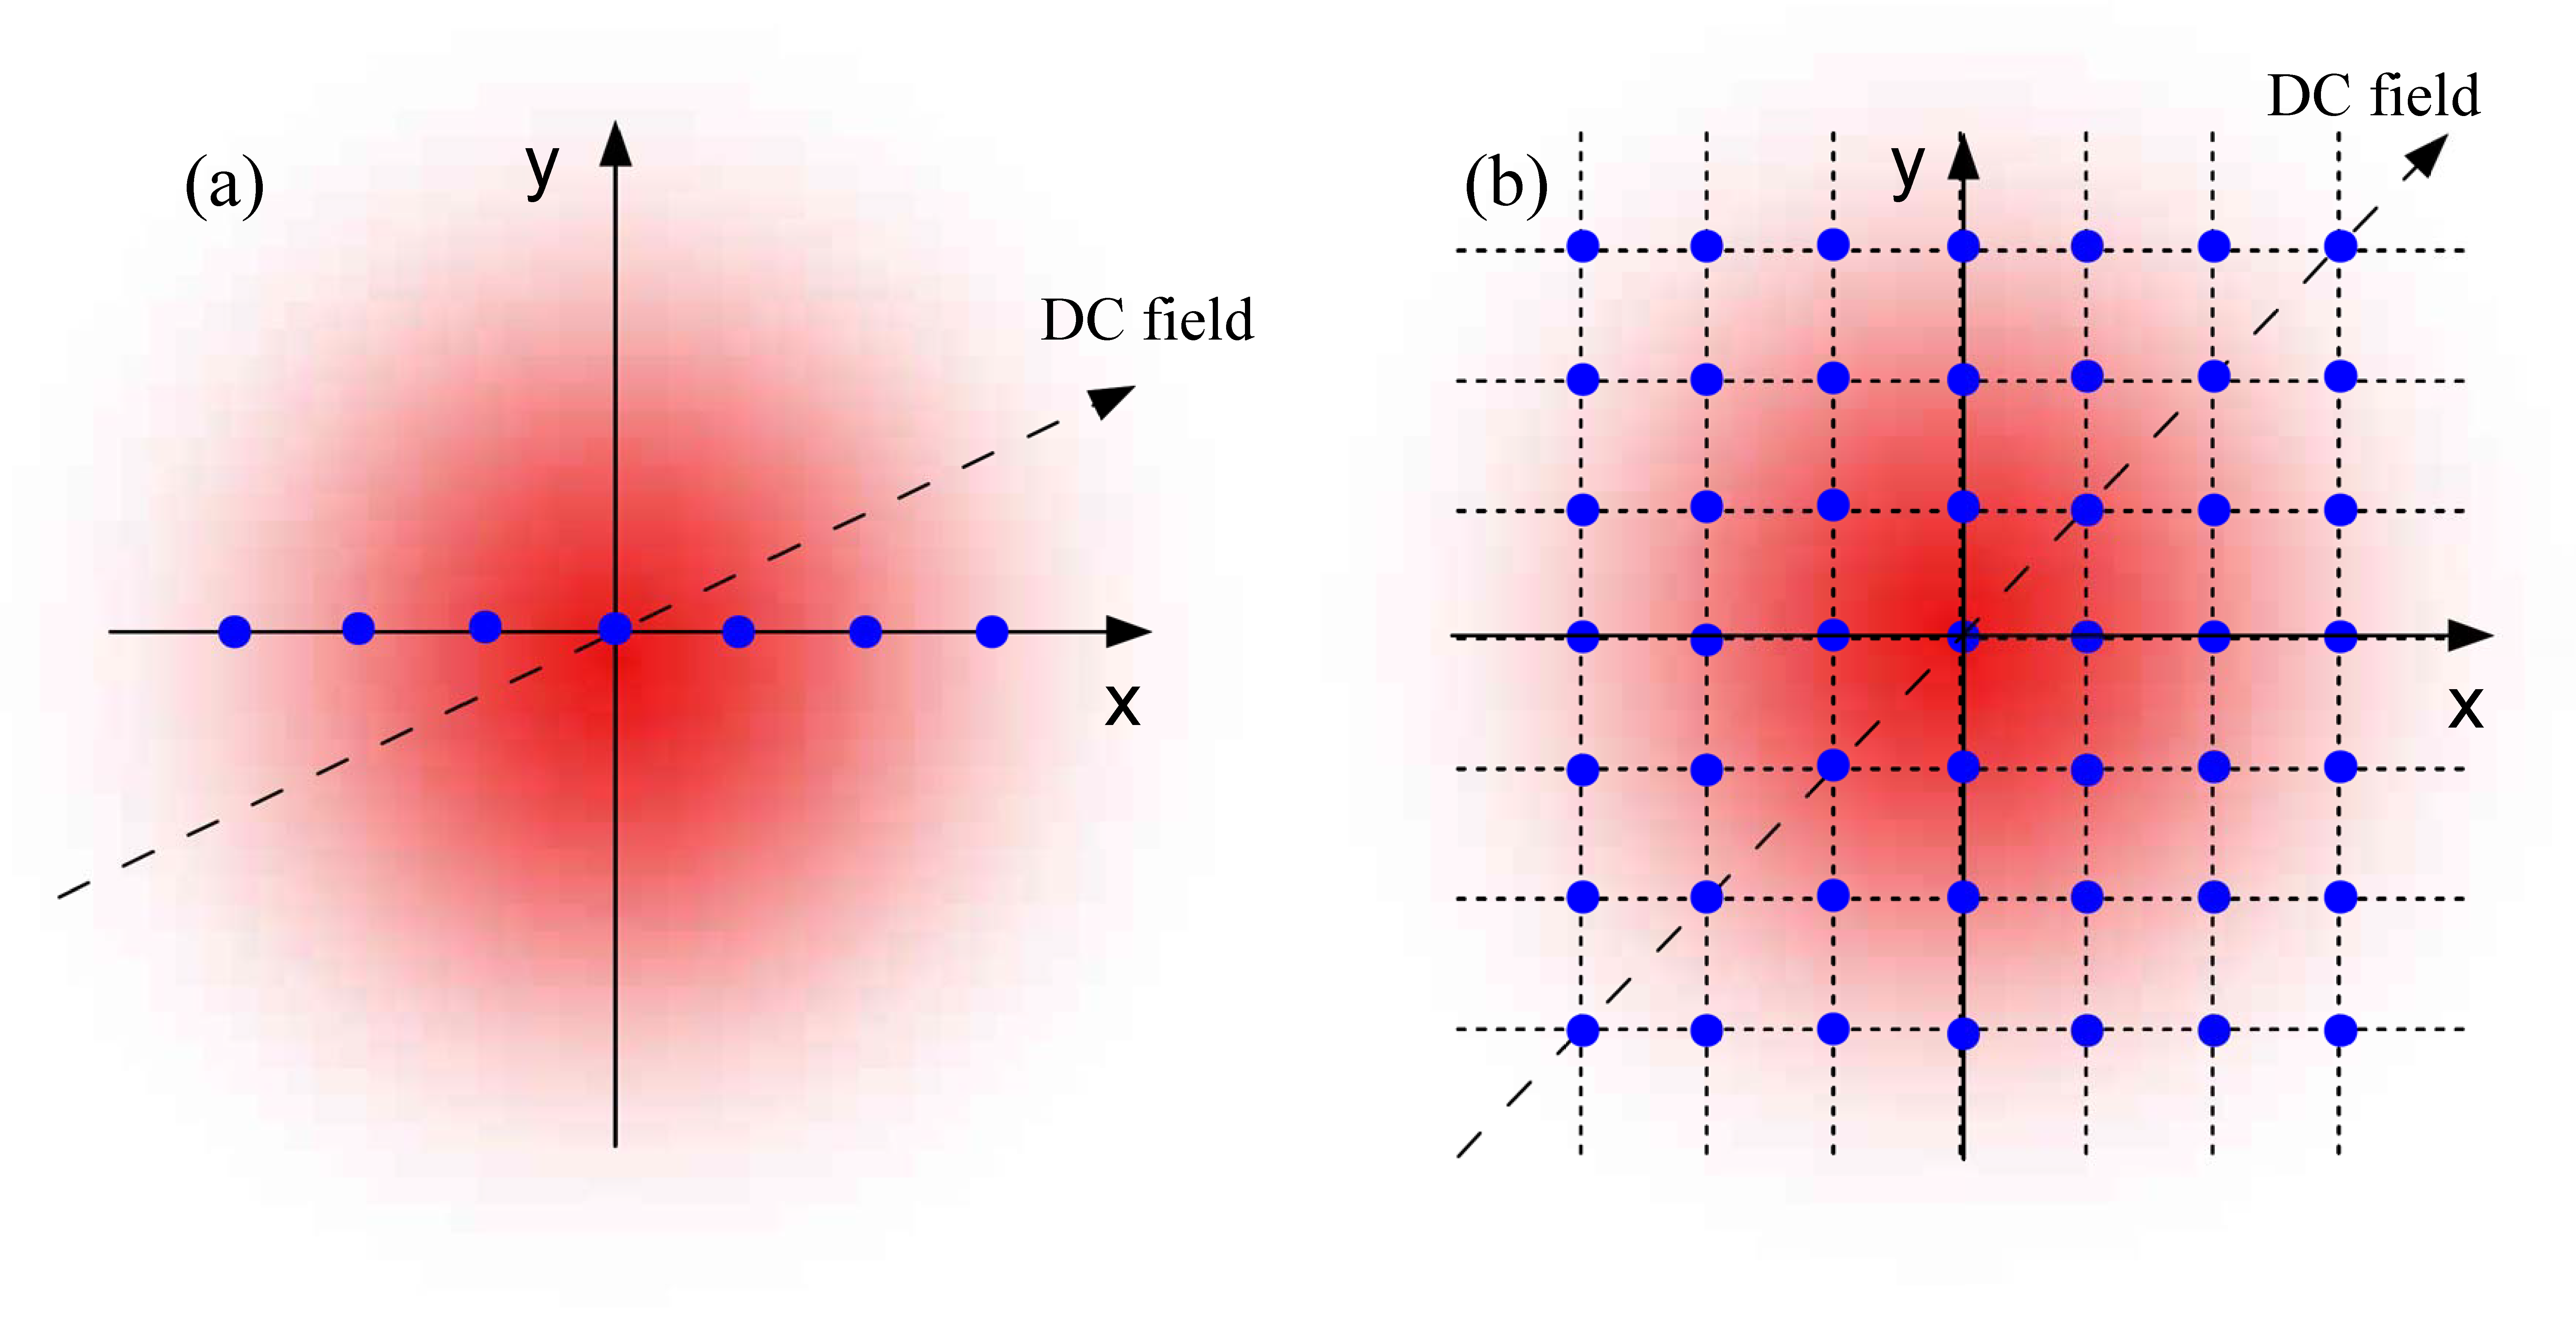
\includegraphics[width=\linewidth]{quadratic-phase-experiment.png}
\caption{An illustration to show the orientations of 1D  and 2D molecular arrays inside the gaussian beam. (a): the
1D lattice lies along the $x$-axis of the $z=0$ plane and the DC field is at some angle with the $x$-axis
such that the coupling $\alpha$ between molecules is negative. (b): the 2D square lattice is at the the center of
the $z=0$ plane and the DC field is at $45^\circ$ degree with the $x$-axis. In both cases, the laser is linearly
polarized along the direction of the DC field.
 }
\label{fig:quadraticExperimentalSetup}
}

First, we consider the case of 1D molecular array. The wave packet that we want to focus is a Gaussian wave packet
with the width $\sigma_x$. 
We put  the beam center at the center of the wave packet and define the $x$-axis of the $z=0$ plane to be along the intermolecular 
axis (see \autoref{fig:quadraticExperimentalSetup} (a)). Then the molecules in the lattice
can be indexed by theirs $x$ coordinates $n_x a$. 
If the dimension of the wave packet is smaller than one third of the
beam waist, we can approximate the gaussian intensity profile in
\autoref{gaussian-intensity-profile} by
\begin{equation}
I(x, y=0, z=0) \approx I_{0}\left(1- \frac{2 n_x^2 a^2}{w_0^2}\right) \ ,  \label{quadratic-profile-1D}
\end{equation}
with an accuracy of 90\%. \Autoref{quadratic-profile-1D} presents a concave quadratic intensity
profile which can be used to focus a wave packet with attractive
coupling ($\alpha < 0$) (see \autoref{sec:wavepacketFocusing}). This indicates that we need to make the coupling 
$\alpha$ between molecules negative. 
A calculation of the dipole-dipole interaction between molecules in DC field shows that $\alpha$ is proportional
to $(1/3 - \cos^2\theta)$ where $\theta$ is the angle between the DC field and the intermolecular axis 
(or $x$-axis). Therefore, we can orientate the DC field to a proper direction to achieve the attractive coupling 
between molecules. As shown in \autoref{control-exciton} (a), $\theta$ must be in the range  $[0, 57.3^{\circ})$
to ensure the attractive coupling. 

From previous
discussions in \autoref{sec:wavepacketFocusing}, we know that good focusing effect occurs when the quadratic 
phase profile applied is $\Phi(n) = \Phi_0 n^2$ with $\Phi_0 = -a/2\sigma_x$ if $\alpha<0$. So we will use this
 particular value of $\Phi_0$ to estimate the power of the laser that are needed for the focusing.  
Specifically, we are using a laser pulse with a short ramp-up and
ramp-down time $T_s$ and a long steady time $T_l$:
\begin{equation}
I_0 (t)=\left\{
\begin{array}{ll}
I_{m}\sin^2\left(\frac{\pi\tau}{2 T_{s}}\right) & (0\le \tau<T_s) \\
I_{m} & (T_s \le \tau \le T_s + T_{l}) \\
I_{m}\sin^2\left[\frac{\pi(\tau- T_s - T_{l}) }{2 T_{s}} +
\frac{\pi}{2}\right] & (T_s+ T_{l}<\tau \le 2T_s+ T_{l})
\end{array}
\right. \label{pulse-profile}
\end{equation}
Based on \autoref{eqn:expressionOfPhase} and \autoref{DressedEnery-Sum}, the phase acquired by a molecule
at site $n_x$ with respect to the molecule at the beam center is given by
\multiline{
\phi(n_x) &=& - \frac{2 (\alpha_{\|}-\alpha_\perp) I_0 n_x^2 a^2} {15 w_0^2}\left( \frac{T_s}{2} + T_{l} \right) \nonumber \\
&\approx& - \frac{2 (\alpha_{\|}-\alpha_\perp) I_0 n_x^2 a^2 T_{l} } {15 w_0^2} \ ,
}
where $T_{l} \ll T_{s}$ is assumed in the last step. Equating $\phi(n_x)$ with the optimal phase profile 
$\Phi(n_x) = \Phi_0 n_x^2 = -a/2\sigma_x n_x^2$,
and assuming the laser power is $P$ and the initial width of the wave
packet is $\sigma_x = S a$, we can estimate the
duration of the laser pulse to be
\begin{equation}
T_l \approx \frac{15 \pi
w_0^4}{4 Sa^2(\alpha_{\|}-\alpha_\perp)P} \ .
\label{pulse-duration}
\end{equation}
For LiCs molecules trapped on a optical lattice with the lattice constant $a = 400 $nm, if the initial width of the 
wave packet is about 100 lattice sites and the beam waist is 3 times larger than that width,  the
pulse duration calculated from Eq. (\ref{pulse-duration}) is about
335 $\mu$s for a laser Gaussian beam with the power of 10 W. To ensure the focusing works
as expected, the wave packet should be exposed to the laser field for long enough time to accumulate the required phases, so the focusing time $T_f$ for the wave packet to become
most focused must be longer than the duration of the laser pulse.
This is not a problem considering that $T_f$ is inversely
proportional to the coupling strength $\alpha$:
\oneline{
T_f \approx \frac{1}{4 \alpha \Phi_0} \ , 
}
and $\alpha$ can be tunned to be very small through changing the magnitude of the DC field
\cite{felipe} by only a few kV/cm or by increasing the angle $\theta$. For instance, when the DC field is about 1 kV/cm and orientate along the intermolecular axis,  the focusing time 
\oneline{
T_f \approx  \frac{1}{4 \alpha \Phi_0} = \frac{1}{4 (-20 \mbox{ kHz}) (-\frac{1}{200})} = 2.5 \mbox{ ms}
}
is much longer than the duration of the laser pulse, leaving enough time for the accumulation of the phases. 

Second, we consider the case of 2D molecular array. The situation is similar to the 1D case except that anisotropy
of the dipole-dipole interaction comes into play. Instead of only considering the coupling between molecules in 
the $x$-axis, we also have to consider the dipole-dipole interactions along $y$-axis and along other directions
between $x$-axis and $y$-axis. This is because the DC field will be at different angles with the different chains of 
molecules, giving rises to different dipole-dipole interactions in different directions. For simplicity, we use the
 nearest neighbor approximation here and only consider
the dipole-dipole interactions along the $x$-axis and $y$-axis. Assuming the dimension of the wave packet is
 smaller than one third of the beam waist, we can approximate the gaussian intensity profile in
\autoref{gaussian-intensity-profile} by
\begin{equation}
I(x, y=0, z=0) \approx I_{0}\left[1- \frac{2 \left(n_x^2 + n_y^2 \right) a^2}{w_0^2}\right] \ .  \label{quadratic-profile-2D} 
\end{equation}
Similar to \autoref{quadratic-profile-1D} in the 1D case, \autoref{quadratic-profile-2D} is also a concave quadratic
 intensity profile which can be used to focus a wave packet with attractive coupling. But the difference here is
 that we need to make sure both the couplings along $x$-axis and $y$-axis are negative. Since the interaction
 along $x$-axis and $y$-axis are independent of each other, the dependence of $\alpha$ on $\theta$ in the 1D
case can be applied for the 2D case. Therefore, in order for the focusing scheme to work, the angle $\theta_x$ 
between the DC field and the $x$-axis and the angle $\theta_y$ between the DC field and the $y$-axis should be
in the range  $[0, 57.3^{\circ})$. As an example, \autoref{fig:quadraticExperimentalSetup} shows one 
configuration $(\theta_x = \theta_y = 45^\circ)$ which will ensure attractive coupling along both axes. 


%%%%%%%%%%%%%%%%%%%%%%%%%%%%%

%With the 1D molecular array arranged along the $z$-axis, the laser field intensity
%can be made to vary nearly linearly along the array,
%\begin{equation}
%I(r=na, z=0; t) \approx [I_{c} + n I_1 ] \, \sin^{2}(\pi t/T) \; \;\; (0 < t <
%T) \ , \label{intensity-varying}
%\end{equation}
%where $I_{c}$ is the intensity at the center of the wave packet.
%This can be achieved if $z_0 = z_R/\sqrt{3}$ and ${\sigma}_x^{(2d)}
%a\lesssim 0.5 z_R$, where $z_0$ is the distance between
%the center of the wave packet and the beam center, and ${\sigma}_x^{(2d)}$ is the width (in the coordinate representation) of the two-dimensional wave packet. Using \autoref{phase}, \autoref{DressedEnery-Sum} and (\ref{gaussian-intensity-profile}), we estimate the momentum kick by such a pulse as $
%%\begin{equation}
%\delta = -\sqrt{3}T I_{0} (\alpha_{\|}-\alpha_\perp) / 80 z_R
%%~. \label{Kick-AC}
%%\end{equation}
%$.
%The results presented in Figure 1 were obtained for a 1D array of LiCs molecules on an optical lattice with $a=400$ nm and the external perturbation
%given by the laser field pulse (\ref{intensity-varying}) with parameters $I_c$ and $I_1$ derived from  \autoref{gaussian-intensity-profile} with $z_0 = 45\; \mu$m and
%$z_R=73.8\; \mu$m. The numerical results deviate from the analytical prediction for $\delta$ by less than 7 \%.

%The Gaussian intensity profile (\ref{gaussian-intensity-profile}) can be used also to implement the quadratic phase transformations needed for focusing of collective excitations. 
%To achieve this, a 2D molecular array must be arranged in the $z=0$ plane,
%with the  $x$-axis defined to be along the polarization direction of a linearly polarized field.
%If the dimension of the molecular array is smaller than one third of the
%beam waist, the Gaussian intensity profile in
%\autoref{gaussian-intensity-profile} can be approximated
%%\tb{``, to better than 90 \%," -- let's cancel it? This may depend on parameters of the system...} 
%by
%\begin{equation}
%I(r=na, z=0; t) \approx I_{0}\left[1- \frac{2(n_x^2 +
%n_y^2)a^2}{w_0^2}\right]. 
%\label{quadratic-profile}
%\end{equation}
%This is a concave quadratic intensity
%profile which can be used to focus a wave packet  in a system with negative couplings $\alpha$ (see \autoref{sec:focusing}).



\section{Control of energy transfer in dipolar systems}
\label{sec:controlEnergyTransfer}

Dipolar interactions play a central role in the study of long-range interaction effects using ultracold systems \cite{our-njp-review}.
While, in general, the coupling constant $\alpha$ in \autoref{ham} can be determined by a variety of interactions, the dominant contribution to $\alpha$ for atoms and molecules on an optical lattice is determined by the matrix elements of the dipole - dipole interaction. It is therefore particularly relevant to discuss the specifics of energy transfer in systems with dipolar interactions. 

\subsection{The effect of long-range interaction}
\label{sec:long-rangeInteraction}

The dipolar interactions are long-range and anisotropic. This long-range character
manifests itself in the modification of the exciton dispersion (\ref{Eexc}). While \autoref{Eexc} is valid for a system 
with nearest neighbour couplings only, higher-order couplings in the case of $\alpha(n-m) \propto 1/ |n-m|^3$ 
modify the exciton dispersion leading to a cosine-like, 
but non-analytic dispersion relation, both in 1D  and 2D. 

To see why the dispersion curve is non-analytic, we start from the expression for $E(k)$:
\multiline{
E (k) &=& \Delta E_{eg} + \sum_{n} \alpha(n) e^{- i k a n} \nonumber \\
&=&  \Delta E_{eg} + \sum_{n} \frac{\alpha}{|n|^3} e^{- i k a n} \ , \label{eqn:dispersionCurveExpression}
}
where $n$ is the difference of two molecular indexes and the summation goes from $-\infty$ to $-1$ and from
$1$ to $\infty$ for a crystal of inifinite size. Restricting $n$ to be a positive integer,
\autoref{eqn:dispersionCurveExpression} can be written as
\multiline{
E (k) &=& \Delta E_{eg} + \sum_{n = 1}^{\infty} \frac{2 \alpha \cos(k a n) }{n^3} \ . \label{eqn:EkPositiveN}
}
Then the first derivative of the dispersion curve is given by
\multiline{
\frac{d E(k)}{d (k a)} = -\sum_{n = 1}^{\infty} \frac{2 \alpha \sin(k a n) }{n^2} \ , \label{eqn:firstDerivative}
}
and the second derivative of the dispersion curve is given by
\multiline{
\frac{d^2 E(k)}{d (k a)^2} = -\sum_{n = 1}^{\infty} \frac{2 \alpha \cos(k a n) }{n} \ . \label{eqn:secondDerivative}
}
The series in \autoref{eqn:EkPositiveN} and \autoref{eqn:firstDerivative} converge with respect to $n$, but the 
series in \autoref{eqn:secondDerivative} doesn't. 
For example, when $k a = 0$ or $\pi$, the series in \autoref{eqn:secondDerivative} becomes the harmonic series and
 it diverges with respect to $n$. 
Therefore, the dispersion curve cannot be taylor expanded as follows:
\multiline{
E(k) = E(k_0) + \left.\frac{d E(k)}{d k}\right|_{k_0} (k - k_0) +  \left.\frac{d^2 E(k)}{d k^2}\right|_{k_0} (k - k_0)^2 + \cdots  \ . \label{eqn:taylorExpansionInvalid}
} 


Conventionally, we only consider the interactions between nearest neighbors and take $n=1$ in
 \autoref{eqn:EkPositiveN}, this might be justified if only a rough estimate of the dispersion curve is wanted
because the series in \autoref{eqn:EkPositiveN} converges very fast with respect to the distance $n$. Given the 
consideration on the convergence, more neighbors should be included in the summation to calculate the properties 
dependent on the first derivative of the dispersion curve, and all neighbors are probably needed to calculate 
properties determined by the second derivative. 


To investigate the effect of this nonanalyticity in dispersion curve, we have performed a series of calculations with the long-range couplings neglected 
after a certain lattice site separation $n-m$ for the 1D system. The results become  converged (to within 0.2 \%) when
 each molecule is directly coupled with 20 nearest molecules. While the calculations with only the nearest neighbor
 couplings are in good agreement  with the analytical predictions given by \autoref{focus-time} and \autoref{x-focusing-Gauss}, the full calculations reveal that long-range 
couplings somewhat decrease the focusing efficiency. The long-range couplings also decrease the focusing time, 
by up to a factor of 2. The dynamics of collective excitations leads to interference oscillation patterns clearly 
visible in panels a and c of Figure \ref{focusing-1d}. These oscillations are much less pronounced when all but nearest
 neighbor couplings are omitted. Given that the analytical derivation in \autoref{sec:focusing} are based on possible 
invalid taylor expansion of dispersion curve (\autoref{eqn:taylorExpansionInvalid}), the numerical results of 
\autoref{focusing-1d} and \autoref{focusing-2d} are particularly important
 because they demonstrate that the phase transformations introduced in the present work are effective  for 
systems with dipolar interactions. 

\subsection{Anisotropy of dipolar interaction}
\label{sec:anisotropy}

The anisotropy of the dipolar interactions can be exploited for controlling energy transfer in dipolar systems by varying the {\it orientation} of a dressing external DC electric field. 
For example,  for polar molecules on an optical lattice,  
the matrix elements  $\alpha(n-m) = \langle e_{n} , g_{m} | {V}_{\rm dd}(n-m) | g_{n}, e_{m} \rangle$ depend not only on the choice of
 the states $|g\rangle$ and $|e\rangle$, but also on the magnitude and orientation of an external dc electric field
\cite{biexcitons, felipe}. Since the value of $\alpha$ determines the exciton dispersion (\ref{Eexc}),
 the exciton properties can be controlled by varying the angle $\theta$ between the intermolecular axis
and the applied DC field. This is illustrated in Figure 4. 

The calculations presented in Figure \ref{control-exciton} are for a 1D array of LiCs molecules in a lattice with  $a=400$ nm.
As before, $|g\rangle$ is the absolute ground state of the molecule and $|e\rangle$ is the rotationally excited state
 that adiabatically correlates
with the rotational state $|J=1, M_J = 0 \rangle$ in the limit of vanishing electric field. 
The upper panel of Figure 4
shows that the angle $\theta$ between the electric field vector and the molecular array axis
determines the sign and magnitude of $\alpha$, and therefore the shape of the dispersion
curve. This enables
control over the sign and magnitude of the group velocity of an
excitonic wave packet containing contributions with $k\neq 0$. Dynamically tuning $\theta$,
one can propagate a localized excitation to different parts of the
lattice, as shown in Figure \ref{control-exciton} (b).

In a 2D lattice, the intermolecular interactions depend on an additional azimuthal angle $\phi$ that describes
 the rotation of the electric field axis around the axis perpendicular to the lattice. The numerical calculations 
presented in Figure \ref{control-2d-wavepacket} show that the energy flow in two dimensions can be  
controlled by varying both $\theta$ and $\phi$. 
In addition to the phase transformation discussed earlier, this allows for a dynamical energy transfer in quantum 
many-body systems with anisotropic interparticle interactions.

\subsection{Numerical details}
\label{sec:numerical}

In this subsection, we show how to carry on the calculations presented in \autoref{sec:anisotropy}. We first evaluate 
dipole-dipole interaction in the 1D and 1D molecular arrays and form the Hamiltonian
matrix, then present some  details about coding. 

As discussed in \autoref{sec::ddInteraction}, the dipole-dipole operator for molecule $A$ and molecule $B$ separated by 
$\vec{R}$ in optical lattices is given by
\oneline{
\hat{V}_{\rm dd}(R) = -2 \sqrt{\frac{6 \pi }{5}} \left( \frac{1}{R} \right)^3 \sum_{q} (-1)^q Y_{2, -q}(\theta_{R}, \phi_{R}) \left[ d_{A}^{(1)} \otimes d_{B}^{(1)}\right]_{q}^{(2)}
}
where the angles $(\theta_{R}, \phi_{R})$ describe the orientation of the vector  $\vec{R}$ in the coordinate
 system whose $z$-axis coincides with the the direction of DC field and $Y_{2, -q}$ are these spherical harmonics:
\multiline{
Y_{2, -2} &=& \frac{1}{4} \sqrt{\frac{15}{2\pi}}\sin^2 \theta_{R} e^{- 2 i \phi_{R}} \nonumber \\
Y_{2, -1} &=& \frac{1}{2} \sqrt{\frac{15}{2\pi}}\sin \theta_{R} \cos \theta_{R} e^{-  i \phi_{R}} \nonumber \\
Y_{2, 0} &=& \frac{1}{4} \sqrt{\frac{5}{\pi}} (3\cos^2\theta_{R} - 1) \nonumber \\
Y_{2, 1} &=& -\frac{1}{2} \sqrt{\frac{15}{2\pi}}\sin \theta_{R} \cos \theta_{R} e^{  i \phi_{R}} \nonumber \\
Y_{2, 2} &=& \frac{1}{4} \sqrt{\frac{15}{2\pi}}\sin^2 \theta_{R} e^{2 i \phi_{R}}
}
To calculate the dipole-dipole interaction, we evaluate the matrix element of the dipole-dipole operator in the basis
of bare rotational states:
\multiline{
&&\bra{N_A , M_A} \bra{N_B , M_B} \hat{V}_{\rm dd}(R) \ket{N_A^{'}, M_A^{'}} \ket{N_B^{'} , M_B^{'} } \nonumber \\
&&= - \frac{F}{2 R^3} \bigg\{ 3\sin^2\theta_{R} e^{-2 i \phi_{R} } D^{A}_{-} D^{B}_{-} - 6\sin\theta_{R}\cos\theta_{R} e^{- i\phi_{R}} \left[ D_0^A D_{-}^B + D_{-}^A D_0^B\right] \nonumber \\
&& \hspace{1.5cm} + 3\sin^2\theta_{R} e^{2 i \phi_{R} } D^{A}_{+} D^{B}_{+} + 6\sin\theta_{R}\cos\theta_{R} e^{ i\phi_{R}} \left[ D_0^A D_{+}^B + D_{+}^A D_0^B\right] \nonumber \\
&& \hspace{1.5cm} + \sqrt{6} (3\cos^2\theta_{R}-1) \left[ D_{+}^A D_{-}^B + D_{-}^A D_{+}^B + D_0^A D_0^B \right] \bigg\} \ , \label{eqn:ddMatrixElement}
}
where $F$ and $D_{S}^{X}$ are given in \autoref{sec::ddInteraction}. In $D_{S}^X$ of \autoref{eqn:ddMatrixElement},  
the superscript $X$  (= $A$ or $B$) denotes molecule $A$ or $B$, and the subscript 
$S$ (= $+$ or $-$ or $0$) indicates $D_{S}^X$ is nonzero only if 
the projection of the rotational quantum number of molecule $X$ changes in a certain way: 
``$+$'' means  
$M_X = M_X^{'} + 1$;  ``$-$'' means
 $M_X = M_X^{'} - 1$; $0$ means $M_X = M_X^{'}$. 
As depicted in \autoref{fig:1Dand2D} (a), rotating the coordinate system around its $z$-axis does not change the 
physical properties of the molecular array as the relative orientation of the the DC field with respect to the
 intermolecular axis remains the same. Therefore we have the freedom to choose
 $\phi_{R} = 0$ in \autoref{eqn:ddMatrixElement} for the 1D molecular array. However, a 2D molecular array has
 many intermolecular axes that are at different angles $(\theta_{R}, \phi_{R})$ with the external field, which means 
one cannot make all $\phi_{R}$ zero by rotating the coordinate system while keeping the relative orientation of 
the external field with respect to the molecular array. So in general we have to consider both $\theta_{R}$ and 
$\phi_{R}$ when calculating the dipole-dipole interaction in a 2D molecular array.

\addfigure{
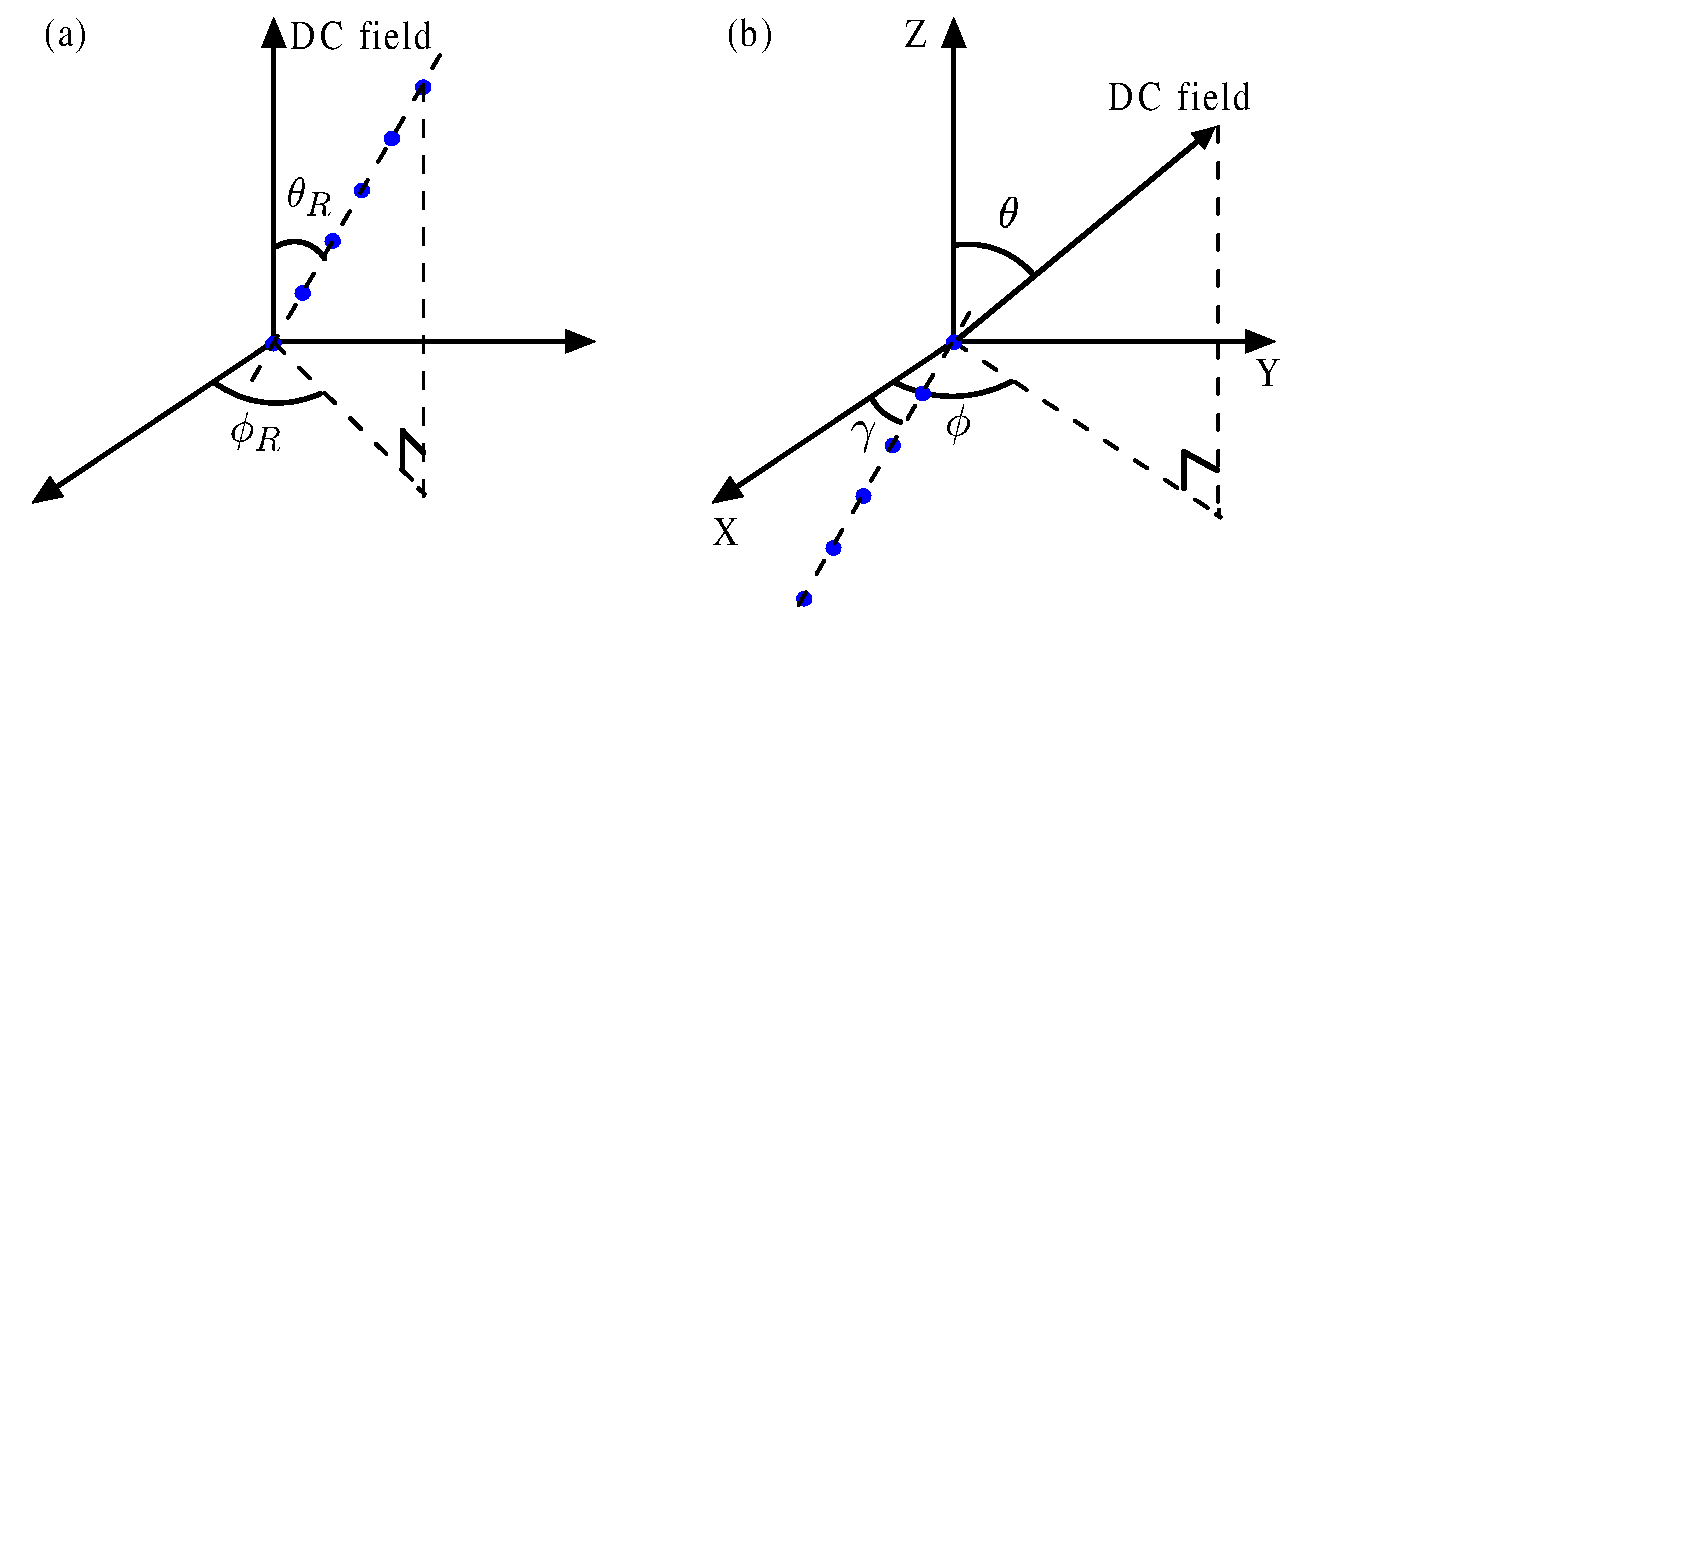
\includegraphics[width=\linewidth]{1Dand2D.pdf}
\caption{The orientations of the DC field and molecular arrays in the coordinate systems. (a): The DC field is along 
the $z$-axis and the 1D molecular array is in the direction represented by $\theta_{R}$ and $\phi_{R}$. (b): The 2D
molecular array is on the $XY$ plane and the orientation of DC field is represented by $(\theta, \phi)$. For clarity,
we have only drawn the molecules (as blue dots) along a particular axis which is at angle $\gamma$ with the $X$-axis.
It is to be understood that there are also other intermolecular axes which are at different angles with the $X$-axis.
Note part (a) and part (b) have different coordinate systems and the meaning of $(\theta_R, \phi_R )$ is different
from that of $(\theta, \phi)$. In fact, the angle $\theta_{R}$ between the DC field and the molecular array in (b)
is related to $\theta$ and $\phi$ by $\cos \theta_{R} = \cos\theta \cos(\phi - \gamma)$. 
 }
\label{fig:1Dand2D}
}

%Based on the meaning of $D_{S}^X$, some terms in 
%\autoref{eqn:ddMatrixElement} will vanish if the projections of the rotational quantum numbers of the initial state
%$ \ket{N_A^{'}, M_A^{'}} \ket{N_B^{'} , M_B^{'} }$ and the final state $\ket{N_A , M_A} \ket{N_B , M_B}$ don't satisfy
%certain conditions. 

Keeping track of both angles $\theta_{R}$ and $\phi_{R}$ is complicated. Fortunately, we can get rid of the 
dependence of $\phi_{R}$ in \autoref{eqn:ddMatrixElement} by choosing to deal with only certain rotational states.  
In a DC field or a linearly polarized laser field, the dressed rotational states $\ket{\Tilde{N}, |M|}$ of the
system is a linear combination of the bare rotational states with the same projection along the direction of DC field 
or along the direction of laser polarization, that is,
\oneline{
\ket{\Tilde{N}, |M|} = \sum_{N} C_{N, M} \ket{N, M} \ .
}
Note that the coefficients $C_{N, M}$ only depend on the magnitude of the external field and have nothing to do  
with the angles $\theta_{R}$ and $\phi_{R}$. 
Because those dressed states with different 
projections $|M|$ have different energies, we can choose to work with the states with a particular value of $|M|$ 
by tunning the excitation energy to just match the corrsponding energy levels. 
In the current study, 
$|M|$ is chosen to be zero, therefore only the bare rotational states with $M_X = 0$ are involved, then only the
term associated with $D_0^A D_0^B$ in  \autoref{eqn:ddMatrixElement} is nonzero, and we have
\oneline{
\bra{N_A , 0} \bra{N_B , 0} \hat{V}_{\rm dd}(R) \ket{N_A^{'}, 0} \ket{N_B^{'} , 0} =  - \frac{\sqrt{6} F}{2 R^3}  (3\cos^2\theta_{R}-1) D_0^A D_0^B \ . \label{eqn:ddM=0}
}
Then the dipole-dipole interaction between two dressed state with $|M| = 0$ can be expressed as a linear combinations of \autoref{eqn:ddM=0}:
\multiline{
&&\bra{\Tilde{N}_A, 0} \bra{\Tilde{N}_B, 0} \hat{V}_{\rm dd}(R) \ket{\Tilde{N}_A^{'}, 0} \ket{\Tilde{N}_B^{'}, 0} \nonumber \\
&& = \sum_{N_A} \sum_{N_B} \sum_{N_A^{'}} \sum_{N_B^{'}} C_{N_A, 0}^{*} C_{N_B, 0}^{*} C_{N_A^{'}, 0}  C_{N_B^{'}, 0} \bra{N_A , 0} \bra{N_B , 0} \hat{V}_{\rm dd}(R) \ket{N_A^{'}, 0} \ket{N_B^{'} , 0} \ .  \nonumber \\ \label{eqn:ddM=0Dressed}
}
\Autoref{eqn:ddM=0} and \autoref{eqn:ddM=0Dressed} show that we only need to consider the angle $\theta_{R}$
between the intermolecular axis and the external field if only the dressed rotational states with $|M|=0$ are
 involved. This is valid for both 1D and 2D cases.  

Since a 1D molecular array can be treated as a limiting case of a 2D molecular array with only a single intermolecular
 axis, we focus on the discussion of the 2D case. As described by \autoref{fig:1Dand2D}, we suppose the 2D molecular 
array is on the $XY$ plane, and the orientation of the external field is presented by $(\theta, \phi)$. For any two 
molecules in the intermolecular axis that are at angle $\gamma$ with the $X$-axis, $\cos^2\theta_{R}$ in
 can be calculated as
\multiline{
\cos^2\theta_{R} &=& \left[\cos\left(\frac{\pi}{2}-\theta\right) \cos(\phi - \gamma)\right]^2 \nonumber \\
&=& \sin^2\theta \left(\cos\phi \cos\gamma + \sin\phi \sin\gamma \right)^2 \ . \label{eqn:threeAnglesRelation}
}
Therefore the dipole-dipole interaction between two molecules can be calculated from \autoref{eqn:ddM=0} and
 \autoref{eqn:ddM=0Dressed} provided that the angle between the intermolecular axis and the $X$-axis is known. 


Once the dipole-dipole interaction is known, we can form the Hamiltonian matrix by expanding the Hamiltonian in 
the basis of individual sites. Suppose the 2D molecular array is a square lattice with $\mathbb{N}\times\mathbb{N}$
sites and the coordinate system is orientated such that its $X$-axis and $Y$-axis coincide with the
bottom and left edge of the 2D lattice respectively, then the position of the
molecule in the array can be represented by its coordinates $(x, y)$. Without the loss of generality, we consider only 
the case where the external field is orientated such that $0\le \theta\le 90^\circ$ and $0 \le \phi \le 90^\circ$, and
give the indexes $0, 1, 2, \cdots, \mathbb{N}^2-1$ to every molecule in the 2D array, starting from the bottom to 
the top of the array and from left to right in each row. Based on \autoref{eqn:ddM=0} and
 \autoref{eqn:ddM=0Dressed},  the matrix element $H_{i,j}$ corresponding to two sites $i$ and $j$ is given by
\multiline{
 H_{i,j} &=& \bra{\Tilde{0},0}_i \bra{\Tilde{1},0}_j H_0 + \hat{V}_{\rm dd} \ket{\Tilde{1}, 0}_i \ket{\Tilde{0}, 0}_j \nonumber \\
&=&  \sum_{N_A} \sum_{N_B} \sum_{N_A^{'}} \sum_{N_B^{'}} - \frac{\sqrt{6} F}{2 R_{i,j}^3}  (3\cos^2\theta_{R}(i,j)-1) D_0^A D_0^B C_{N_A, 0}^{*} C_{N_B, 0}^{*} C_{N_A^{'}, 0}  C_{N_B^{'}, 0} \ , \nonumber \\ \label{eqn:hij2D}
}
where $R_{i,j}$ is the distance between molecule $i$ and $j$, and $\theta_{R}(i,j)$ is angle between the external field
and the intermolecular axis. Assuming the unit length of the coordinate system is the lattice constant of the 2D array,
then the distance between the two site $i$ and $j$ can be calculated from their coordinates
\oneline{
R_{i,j} = a \sqrt{(x_i - x_j)^2 + (y_i - y_j)^2} \ ,
}
where
\multiline{
x_i &=&  i \% \mathbb{N} \nonumber \\
y_i &=& i/\mathbb{N} \ .
}
Since the angle $\gamma$ between the external field and the 
intermolecular axis connecting from molecule $i$ to molecule $j$ is given by
\oneline{
\gamma(i, j) = \arccos\left[ \frac{x_j - y_i }{\sqrt{(x_i - x_j)^2 + (y_i - y_j)^2} } \right] \ ,
}
the value of $\cos^2\theta_{R}(i,j)$ in \autoref{eqn:hij2D} can be calculated from \autoref{eqn:threeAnglesRelation}.

With the Hamiltonian matrix $H$, we can now run the simulations presented in \autoref{sec:anisotropy}. The 
essential problem is to solve the time-dependent Schr{\"o}dinger equation
\oneline{
\dot{\Psi}(t) = \frac{1}{i\hbar} H(t) \Psi(t) \ . \label{eqn:tdse2d}
} 
Solving the above differential equations  involves the computation of the Hamiltonian matrix at many different 
time points. To make the simulation as fast as possible,we now explore how to evaluate $H(t)$ efficiently.
In the calculations, we change the direction of the DC field adiabatically with respect to the time scale of excitation
 hopping while keeping the magnitude of the field, therefore the coefficients $C_{N_A, 0}$, $C_{N_B, 0}$, $C_{N_A^{'}, 0}$, and $C_{N_B^{'}, 0}$ in \autoref{eqn:hij2D} will remains the same and the time dependence of
the Hamiltonian matrix is solely due to the time dependence of $\theta_{R}(t)$. Based on this observation, we can
separate the Hamiltonian matrix into two parts: 
\oneline{
H(t) = H_{1}(\theta(t), \phi(t) ) * H_{2} \ ,
}
where  ``*'' means element-wise multiplication, $H_{1}$ is the time-dependent part that needs to be 
updated whenever $\theta(t)$ and $\phi(t)$ change, and $H_{2}$ is the time-independent part that can be 
computed once and be saved into memory for later retrieve. It is easy to derive from 
 \autoref{eqn:hij2D} the expression of $H_2$:
\oneline{
H_{2} = \sum_{N_A} \sum_{N_B} \sum_{N_A^{'}} \sum_{N_B^{'}} - \frac{\sqrt{6} F}{2 R_{i,j}^3} D_0^A D_0^B C_{N_A, 0}^{*} C_{N_B, 0}^{*} C_{N_A^{'}, 0}  C_{N_B^{'}, 0} \ .
}
Because of the angle $\gamma$ in \autoref{eqn:threeAnglesRelation} is only dependent on positions of the lattice sites, we can further separate the evalulation of $H_1$ into different parts for the purpose of computing efficiency. The expression of $H_1$ is given by
\oneline{
H_{1}(\theta(t), \phi(t) ) = 3\cos^2[\theta(t) ]*\bigg\{\cos[\phi(t)]*K^{\cos} + \sin[\phi(t)]*K^{\sin} \bigg\}**2 - 1
}
where ``**2'' means element-wise square, and $K^{\cos}$ is a matrix whose elements is given by 
\oneline{
K^{\cos}_{i, j}= \cos\left(\gamma(i, j)\right) \ ,
}
and $K^{\sin}$ is a matrix whose elements is given by 
\oneline{
K^{\sin}_{i, j}= \sin\left(\gamma(i, j)\right) \ . 
}
Since $K^{\cos}$ and  $K^{\sin}$ are independent of time, we compute them once and save them into memory 
for later usage. In summary, the efficient computation of $H(t)$ is carried on in three steps: 1. calculate $H_2$, 
$K^{\cos}$, and $K^{\sin}$ and save them into memory; 2. compute $\theta(t)$ and $\phi(t)$ and then use
the values of $K^{\cos}$, and $K^{\sin}$ in memory to calculate $H_1$; 3. use the value of $H_2$ in memory to 
compute $H$.  

In the simulation, I have used a complex ordinary differential equation solver called ``ZVODE'' to solve 
\autoref{eqn:tdse2d}. Given an initial state $\Psi(t=0)$, the
derivative $\dot{\Psi}$ of the wavefunction with respect to time, and the desired accurary for the calculation,
the solver can give the wavefuntion $\Psi(t)$ at a later time $t$. In my experience, the ZVODE solver is not 
good at solving a stiff system of differential equations where the potential change is very steep. 
If this is the case, it is better to convert
the time-dependent Schr\"odinger equation into a real  ordinary differential equation and use the corresponding
ODE solver called ``DVODE'' that can handle stiff systems much better. As a reference
 for future students, we show below the conversion from the time-dependent Schr\"odinger equation to a real 
ordinary differential equation. 

%%%%%%%%%%%%%%%%%%%%%%%%%%%%%%%%%%%%%%%%%%%%%%%%%%%%%%%%%
\begin{figure}[htbp]
\centering
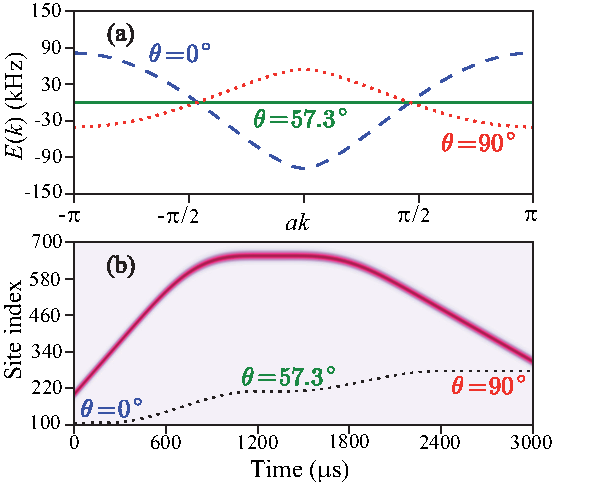
\includegraphics[width=\linewidth]{control-exciton.pdf}
\caption{ Control of excitation transfer in a 1D many-body system with dipolar interactions by varying the 
direction of an external electric field.
Panel (a): Exciton dispersion curves for a 1D
ensemble  of diatomic molecules on an optical lattice for
different angles $\theta$ between the direction of the external DC
electric field and the axis of the molecular array.  In 1D, the coupling $\alpha\propto (1/3 - \cos^2\theta)$.  Panel (b):
Propagation of a wave packet centered at $ak =-\pi/3$ controlled
by tuning the electric field direction. Thin dotted line depicts
the corresponding angle variations with time. The brightness
of color corresponds to the probability of the excitation. }
\label{control-exciton}
\end{figure}
%%%%%%%%%%%%%%%%%%%%%%%%%%%%%%%%%%%%%%%%%%%%%%%%%%%%%%

%%%%%%%%%%%%%%%%%%%%%%%%%%%%%%%%%%%%%%%%%%%%%%%%%%%%%%%%%
\begin{figure}[htbp]
\centering
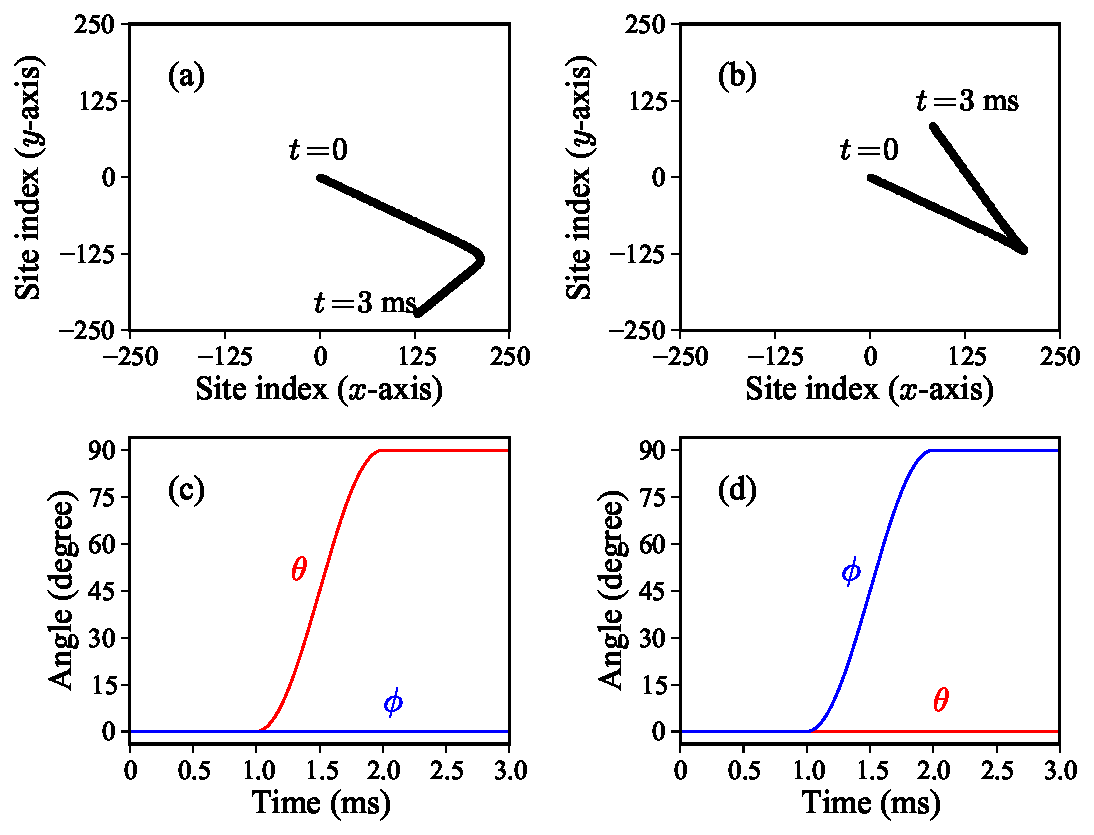
\includegraphics[width=\linewidth]{control-2d-wavepacket.pdf}
\caption{ Control of excitation transfer in a 2D many-body system with dipolar interactions by varying the 
direction of an external electric field.
Panels (a) and (b) show the trajectories of the center of an exciton wave packet in a 2D lattice during
 the time from 0 to 3 ms; Panels (c) and (d) represent the changing of the dressing DC field orientation $(\theta, \phi)$ associated with (a) and
(b) respectively. The initial wave packet is a 2D Gaussian distribution centered around $ak_x=ak_y=\pi/2$ and has a width of $\sim$60 lattice sites in coordinate space. The magnitude of the DC field is fixed to
6 kV/cm while its direction is changing. The calculations are done for a 2D array of  LiCs molecules in a lattice with
$a=400$ nm.
 }
\label{control-2d-wavepacket}
\end{figure}
%%%%%%%%%%%%%%%%%%%%%%%%%%%%%%%%%%%%%%%%%%%%%%%%%%%%%%

\section{Energy transfer in the presence of vacancies}
\label{sec:energyTransferVacancy}

While experiments with ultracold atoms have produced states with one atom per lattice site with  99\%  fidelity \cite{atom-mott1, atom-mott2, atom-mott3},
the latest experiments with molecules yield lattice-site populations about  10\% \cite{Ye-arrays-PRL12}.
Multiple experiments are currently underway to  trap polar molecules on an optical lattice with close to the full population of the lattice.
However, lattice vacancies may be unavoidable in the best experiments. In this section, we examine the effect of vacancies on the possibility of focusing collective excitations
to a desired region of the lattice by the phase transformations discussed in \autoref{sec:focusing}. For concreteness, we perform calculations for the system described in \autoref{sec:excitationAtomMolecule},
namely a 2D array of LiCs molecules on a square optical lattice with $a=400$ nm.



To explore the effect of vacancy-induced interactions, we performed simulations for
different vacancy numbers using the same parameters for molecule-field and inter-molecular interactions as
in the calculations presented in Figure \ref{focusing-2d}b. For each vacancy concentration, we carried out 48
calculations with random distributions of empty lattice sites. The quadratic phase transformations are applied,
as described in \autoref{sec:focusing}, in order to focus the collective excitation at time $t_{\ast}$ to
the molecule in the middle of the 2D array.

Vacancies disturb the translational symmetry of the system and produce an effective disorder potential that tends to
localize collective excitations \cite{perez-rios2010}.
 Because the natural time evolution of the wave packet in a disorder potential may lead to enhancement of the probability in certain
regions of the lattice, it is necessary to distinguish the effect of the vacancy-induced localization and the effect of the focusing phase
transformation. To quantify these two effects, we define two factors:
the enhancement of the probability at the target molecule with respect to the initial value,
\begin{equation}
\eta = \frac{p' (t=t_{\ast})}{p(t=0)},
\label{eta}
\end{equation}
and the ratio of the probability to find the excitation on the target molecule with ($p'$) and without ($p$) the focusing
phase transformation,
\begin{equation}
\chi = \frac{p' (t=t_{{\ast}})}{p (t=t_{ {\ast}})}.
\end{equation}
The time $t_*$ is the focusing time found numerically for the corresponding vacancy-free system.
 The quantity $\eta$ illustrates the actual enhancement of the probability to focus a collective excitation,
while the quantity $\chi$ illustrates the effect of the focusing phase transformation.
Figure 6 presents the values of $\eta$ and $\chi$ as functions of the vacancy concentration.
It illustrates two important observations. First, the disorder potential with vacancy concentrations $> 20$ \%
renders the phase transformation ineffective. In the presence of strong disorder, the dynamics of the system is entirely
determined by the disorder potential and the energy transfer becomes highly inefficient (however, see \autoref{sec:focusingStrongDisorder}). On the other hand, vacancy
concentrations of less than 10 \% appear to have little effect on the efficacy of the focusing phase transformation.

Our calculations indicate that the focusing time may be somewhat modified by the disorder potential, even if the
 concentration of vacancies is less than 10 \%.  Figure 7 depicts the excitation wave functions
 at the time of the maximal enhancement on the target molecule, chosen as molecule (71,71).  Figure \ref{focusing-with-vacancy} shows that
despite the presence of multiple vacancies, the focusing transformation enhances the probability to find the
excitation on the target molecule by 16 times.


% As you can see from Figure \ref{enhancement-vs-vacancy}, the enhancement factors decrease exponentially as vacancy percentage increases, but still a relatively good focusing can be achieved with 10\% of vacancies.

\begin{figure}[htbp]
\centering
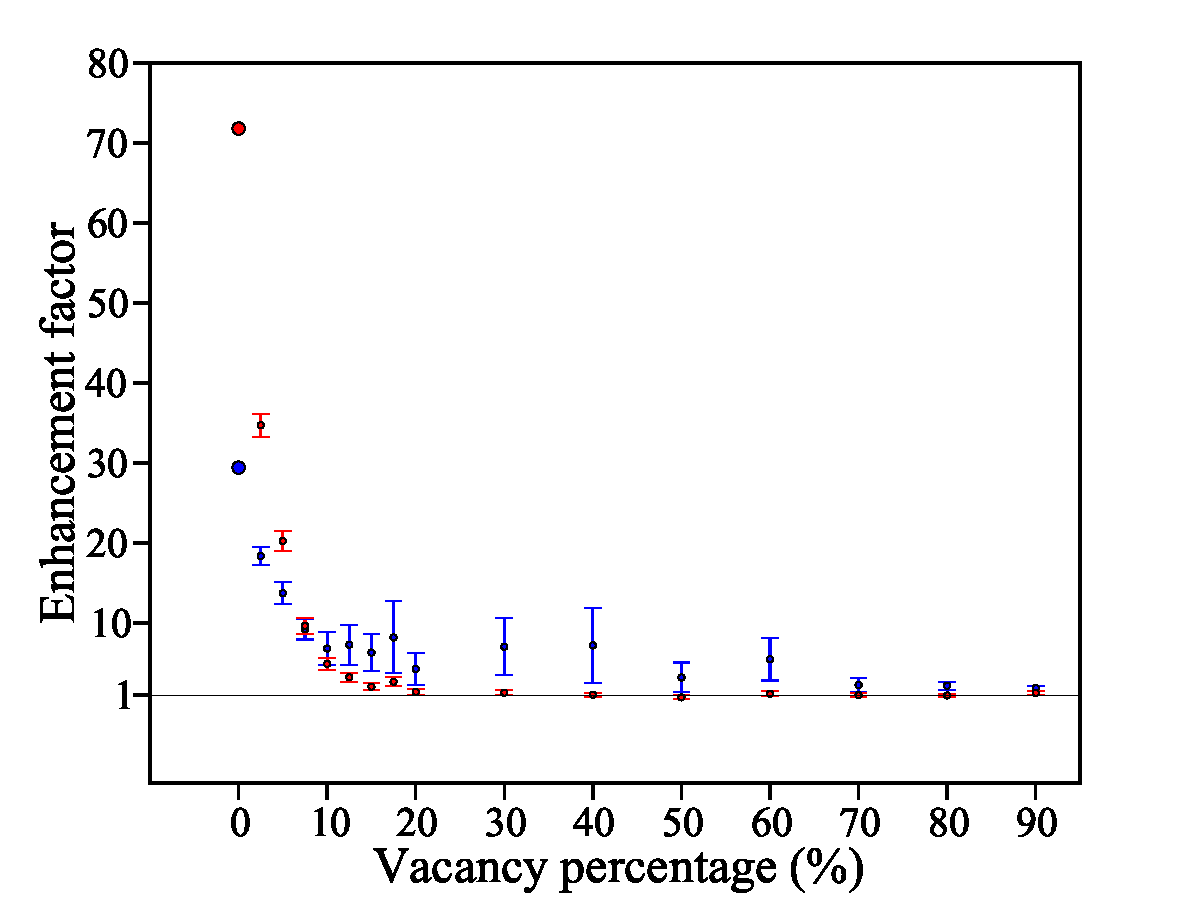
\includegraphics[width=\linewidth]{enhancement-vs-vacancy.pdf}
\caption{ Enhancement factors $\eta$ (red symbols) and
$\chi$ (blue symbols) as functions of vacancy percentage in a 2D lattices. See text
for the definitions of $\eta$ and $\chi$. The error bars are for 95\% of confidence interval. 
} 
\label{enhancement-vs-vacancy}
\end{figure}

%Due to the presence of vacancies in optical lattices, the focusing time $T_{\tiny \mbox{target}}$ for a full lattices would not be the focusing time for a partial lattices. So it is a little unfair to use  $T_{\tiny \mbox{target}}$ as the time for comparison in Figure \ref{enhancement-vs-vacancy} and actually the focusing, as shown in Figure \ref{focusing-with-vacancy},  can be better if the real focusing time is chosen.



\begin{figure}[htbp]
\centering
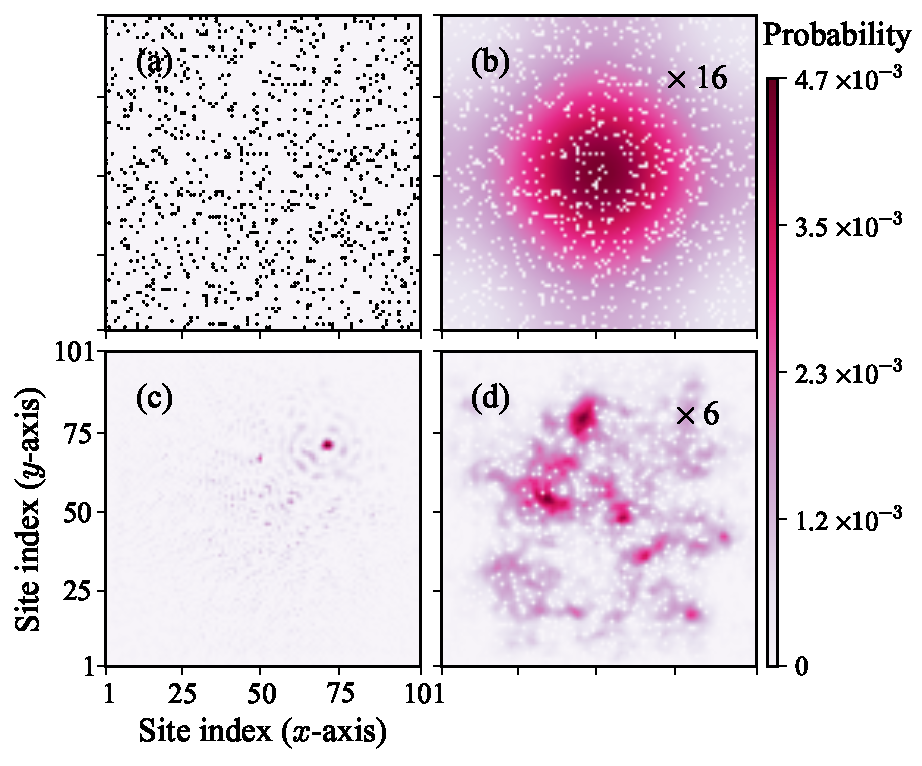
\includegraphics[width=\linewidth]{focusing-with-vacancy.pdf}
\caption{  Time snapshots of a collective excitation in a 2D
array with a vacancy concentration of 10 \%  (a) The distribution of the vacant sites; (b) The initial probability distribution of the excited state; (c) The probability distribution of the excitation at the
focusing time when the focusing scheme is applied. The focusing
time is  found numerically as  the time when the probability at the target
molecule (71, 71) reaches maximum  for a given phase transformation. (d) The probability
distribution of the wave function at the focusing time when the
focusing scheme is not applied. The calculations are performed
with the same parameters as in Figure \ref{focusing-2d}. The
probabilities in (b) and (d) are magnified by 16 and 6
respectively. } \label{focusing-with-vacancy}
\end{figure}

\section{Focusing in the presence of strong disorder}
\label{sec:focusingStrongDisorder}

%\tb{We need to cite something about t-matrix focusing. Zhenia, could you insert citations into the following paragraphs? }

Although the focusing method demonstrated in \autoref{sec:focusing} and \autoref{sec:energyTransferVacancy} appears to be robust in the presence of a disorder potential induced by a small concentration of vacancies, it is important for practical applications to also consider controlled energy transfer in quantum arrays under a strong disorder potential. To consider focusing in a strongly disordered system, 
we employ an analogy with the {``transfer
matrix'' methods for focusing of a collimated light beam in opaque
medium \cite{opaque-1, Gigan-TMeasure-PRL10, Mosk-NPhot10, Cizmar-NPhot10, Silberberg-11, Chatel-Focusing-11, Lagendijk-Focusing-11, zhenia-11, cui-11, kim-11}}.


In optics, a collimated laser beam passing through an opaque medium results in a random
pattern of speckles arising from random scattering of light inside the medium
\cite{RandomWave-books}. Likewise, the random distribution of empty sites in an optical lattice with molecules 
scatters the exciton wavepackets, resulting in a completely random excited state. 
However, in optics, the randomness of the scattering centers inside the opaque medium can be compensated for by
shaping the incident wavefront with a spatial light modulator such
that the contributions from various parts of the medium can add
constructively upon exit from the medium, producing a focus. 
We suggest that the same can be achieved with a many-body system on a lattice by 
separating the entire lattice into multiple blocks and applying proper phase transformations
to those individual blocks. 



%Here we consider an \tz{initial state} \tb{[I like this $|i\rangle$-notation, but probably we should use instead $c_i(t=0) |e_i\rangle \prod_{j\neq i} |g_j\rangle$ to simplify the comparison with Eq.(2)?]}
%plane-wave like initial state with the same probability for each
%occupied site and zero probability for each vacancy site:
%

The initial state for an ensemble of molecules on a lattice with multiple vacancies can be written as 
\begin{equation}
|\psi(t=0)\rangle = \sum_{i}c_i(t=0)|i\rangle \ , \label{planewave-initial}
\end{equation}
where 
\begin{eqnarray}
| i \rangle = |e_i\rangle \prod_{j\neq i} |g_j\rangle
\end{eqnarray}
and the indexes $i$ and $j$ run over all occupied sites. After a long evolution time $T$, the probability amplitude for the excitation to reside on a particular target molecule is given by  
\begin{equation}
c_{o}(T) = \sum_{i} U_{o, i}(T)c_i(t=0) \equiv \sum_i c_{oi}(T), 
\label{site-contribution}
\end{equation}
where $U_{o,i}(t) = \langle o| \exp[-iH_{\rm exc}t] | i \rangle$ is a matrix element of the time evolution operator.
%
{In a disordered system, the transfer coefficients $U_{o, i}$
are not a-priori known and depend on the
disorder potential. The {phasors} $c_{oi}(T)$ have quasi-random
amplitudes and phases. While the amplitude of each phasor cannot be controlled experimentally, 
their phases are controllable via the phases of the coefficients $c_i$ at $t=0$, which can be tuned using the phase-kicking
transformations introduced above.} To achieve the highest probability
at the target molecule, it is necessary to ensure that the contribution
$c_{oi}=U_{o, i}(T)c_i(t=0)$ from every site $i$ has the same
phase so that they add up constructively.

In a practical implementation, it may be difficult to control the phase of each molecule in each
individual site. It may be more desirable to work with blocks of several lattice sites. Assuming that the entire array of molecules 
can be divided into $M$ blocks, each containing many molecules, and that the blocks can be perturbed individually, the excitation probability amplitude at the target molecule at time $T$ is 
%\tz{Let us divide the whole array into $N$ blocks (``channels''), each containing many molecules, in such a way that it is possible to apply an overall phase to molecules in one block without perturbing the others. The excitation at the target molecule at time $T$ is}
%
\begin{equation} c_{o}(T) =  \sum_{\gamma=1}^M c_{\gamma}(T)
\label{blocks-contribution}
\end{equation}
%
where
%
\begin{equation} c_\gamma(T) \equiv |c_\gamma| e^{i\phi_\gamma}= \sum_{i\in
 \gamma} U_{o, i}(T)c_i(t=0) \ .
\label{inblock-contribution}
\end{equation}
%
%
%So we work with sub-blocks of lattice sites and Eq.v(\ref{site-contribution}) becomes
%\begin{equation}
%c_{o}(T) = \sum_{M} \tilde{U}_{o, M}(T)b_M(t=0) \ , \label{block-contribution}
%\end{equation}
%where $M$ is the index for the sub-blocks, and $b_M$ is the vector whose components are coefficients $c_j$'s of sites insidethe sub-block $M$:
%\begin{equation}
%b_M(0) =\left(
%   \begin{array}{c}
%   c_1^{M}(0) \\
%   c_2^{M}(0) \\
%  \cdot \\
%  \cdot \\
%  \cdot \\
%  c_n^{M}(0)
%   \end{array}
%\right) \ , \label{block-coeff}
%\end{equation}
%tz{rewrite in conventional math notations from here} and the element $\tilde{U}_{o, M}$ of the new time evolution matrix  is related to $U_{o, i}$ by the following equation:
%\begin{equation}
%\tilde{U}_{o, M} = \left( U_{o, j}, U_{o, k}, \cdots, U_{o, r}\right) \ , \label {block-evolution0}
%\end{equation}
%where sites $j, k, \cdots, r$ belong to the sub-block $M$. We can rewrite Eq. (\ref{block-evolution0}) as
%\begin{equation}
%\tilde{U}_{o, M} = \left( U_{o, 1}^M, U_{o, 2}^M, \cdots, U_{o, n}^M\right) \ , \label {block-evolution}
%\end{equation}
%to emphasize that all the components are related to occupied sites in sub-block $M$.Substituting Eq. (\ref{block-coeff}) and (\ref{block-evolution}) into Eq. (\ref{block-contribution}), we have
%\begin{equation}
%c_{o}(T) = \sum_{M} c_M(T) \ ,
%\end{equation}
%where each block contributes
%\begin{equation}
%c_M(T) = \sum_{j=1}^{n} U_{o, j}^M (T) c_j^{M}(0) = |c_M| \exp(i
%\phi_{M}) \ . \label{cM}
%\end{equation}
This equation implies that the contributions
from different blocks can be made to interfere constructively by adding
 a phase $\exp(-i \phi_{\gamma})$ to each occupied site in block
 $\gamma$. For $M$ blocks in the array and quasi-random evolution matrix, simply setting all the phases equal
 must lead to $\sim M$-fold increase of the excitation probability at the target molecule, as compared to
 a sum of $M$ quasi-random phasors in \autoref{blocks-contribution} \cite{opaque-1}.

Similarly to optics, the phases $-\phi_\gamma$ which must be added in each block, can be found experimentally provided
that the same (or similar) realization of disorder persists in a series of
trials. A straightforward optimization would scan through the
strengths of  phase kicks applied to different blocks. In each
experiment one would measure the excitation probability at the
target molecule $|c_o(T)|^2$, e.g. via resonance fluorescence from
the target molecule at the end of the experiment. More
sophisticated optimization techniques, aimed at fast focusing
multi-frequency light in optical systems, are currently under
rapid development \cite{Gigan-TMeasure-PRL10, Mosk-NPhot10, Cizmar-NPhot10, Silberberg-11, Chatel-Focusing-11, Lagendijk-Focusing-11, zhenia-11, cui-11, kim-11}.


%\tz{However, numerically we find the phases $\phi_M$ in a faster way.{ CONSULT WITH PING WHETHER WHAT IS BELOW IS EXACTLY WHAT HE DID IN THE CALCULATION}} 

For a proof-of-principle calculation, we consider a 2D lattice of size 101$\times$101 with 60\% of sites vacant and each non-vacant site occupied by a single LiCs molecule. 
Due to time reversibility of the time
evolution operator $U(T)$, 
%the phase $\exp(-i \phi_{M})$ can be obtained as follows:
\begin{equation}
|c_\gamma | \exp(-i \phi_{\gamma}) = \left[ \sum_{j=1}^{n} U_{o, j}^\gamma (T) c_j^{\gamma}(0)\right]^* 
=\left[ \sum_{j=1}^{n} U_{j, o}^\gamma (-T) c_j^{\gamma}(0)\right]^* \ .
\end{equation}
The matrix element $U_{j, o}^\gamma (-T)$ can be
calculated by performing a backward time propagation starting from a
local excitation at site ``$o$'' and calculating the coefficient
$c_j(t)$ at time $-T$. Alternatively, one can propagate the evolution equations forward in time, finding $c_j(T)$: 
Since the Hamiltonian (1) is real, its eigenfunctions are real, and the evolution matrix $U$ is symmetric, $U_{o, j} = U_{j, o}$. Thus we find
\begin{equation}
c_j(T) = \sum_{i}U_{j, i}^\gamma (T) c_i(0) = U_{j, o}^\gamma (T) \ ,
\end{equation}
since $c_{o}(0) = 1$ and all other coefficients are zero. For a completely delocalized initial state, we assume that all coefficients
in auto\ref{planewave-initial} are equal, so that  the phases $\phi_\gamma$ required for
block $\gamma$ are
\begin{equation}
 |c_\gamma|\exp(- i \phi_{\gamma})  = \left[ \sum_{j}  c_j(T) \right]^* \ , \label{phase-applied}
\end{equation}
where the index $j$ runs over all  occupied sites in block $\gamma$.
Figure \ref{t-matrix-focusing} shows that this choice of phases leads to effective focusing of the collective excitation in a strongly disordered system. 

\begin{figure}[htbp]
\centering
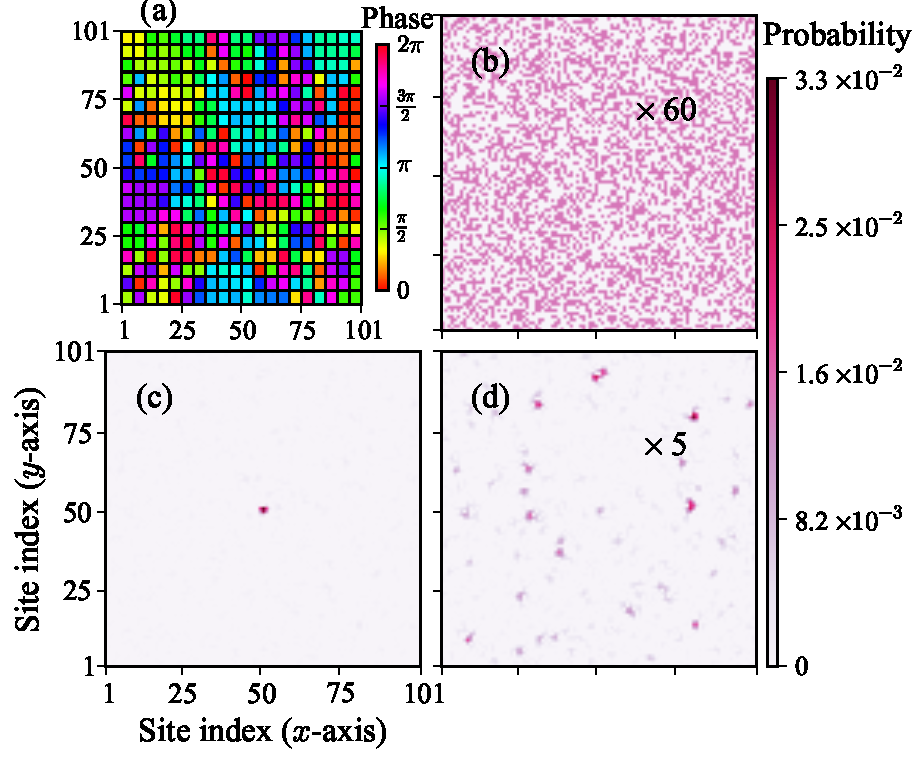
\includegraphics[width=\linewidth]{t-matrix-focusing.pdf}
\caption{  Focusing of a collective excitation in a strongly disordered system with 60\% of lattice sites unoccupied.  Panel (a) shows different phases applied to
different blocks of the lattice before the time evolution.
(b) The initial probability distribution of the excited state. (c) The probability distribution of the excited state at the
focusing time $T = 3$ ms with the phase transformation depicted in panel (a) before the time
evolution. (d) The probability distribution of the excited state at the focusing time $T = 3$ ms with no phase transformation
applied. The calculations are performed
with the same parameters as in Figure \ref{focusing-2d}. The
probabilities in (b) and (d) are magnified by 60 and 5,
respectively. } \label{t-matrix-focusing}
\end{figure}


To illustrate the efficiency of the focussing method described above, we have carried out a series of calculations 
with different vacancy concentrations. For each vacancy concentration, we performed 48 calculations with random
 distributions of empty lattice sites. The phase transformations are calculated individually for each random 
distribution of vacancy sites as described above. The results are shown in Figure \ref{enhancement-vs-vacancy-t-matrix}. 
As can be seen, the transformations proposed above are effective for vacancy concentration $<$ 70\%. At higher 
concentrations of vacancies, the excited states become strongly localized and immobile. The focusing efficiency at
vacancy concentrations 10\% and 20\% appears to be higher than that in the absence of vacancies, which we attribute to the effect of 
the boundaries.
\begin{figure}[htbp]
\centering
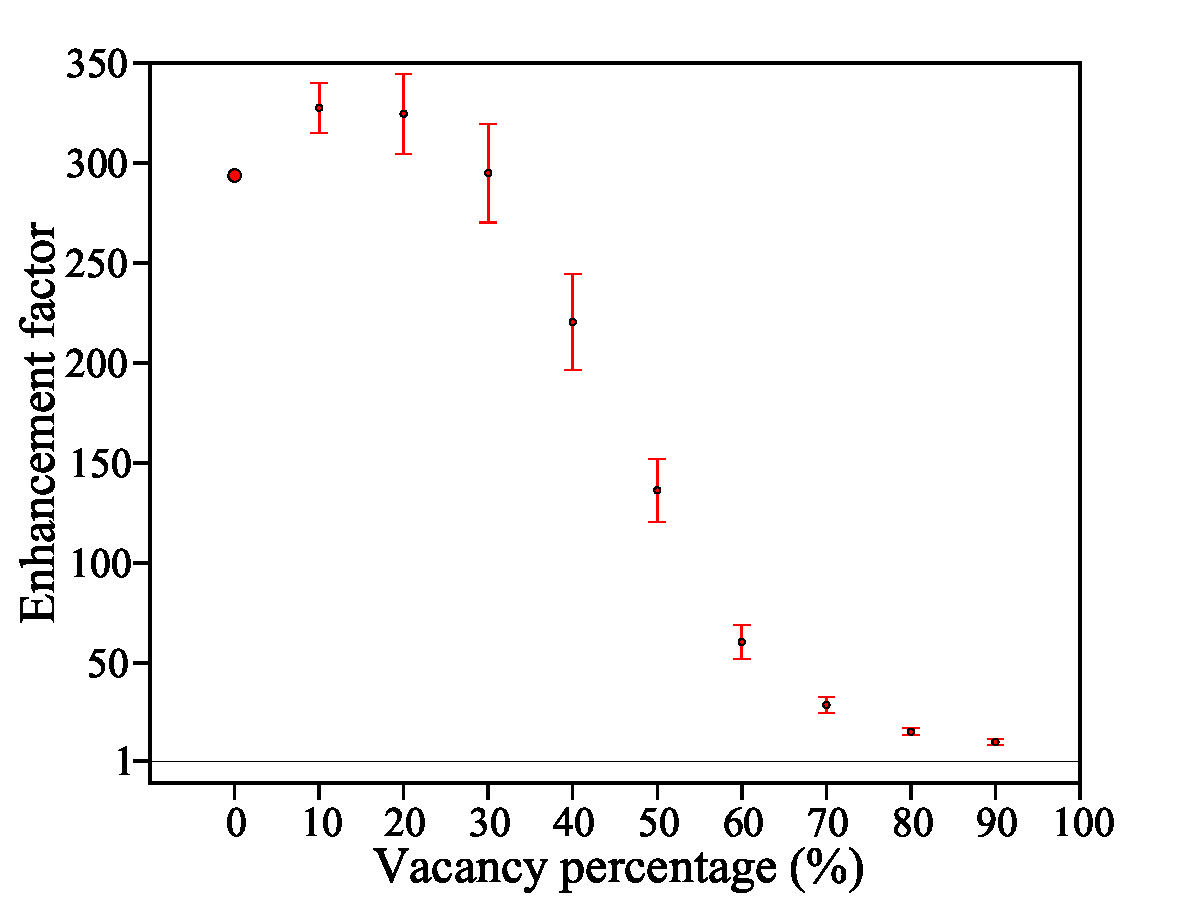
\includegraphics[width=\linewidth]{enhancement-vs-vacancy-t-matrix-other.pdf}
\caption{Efficiency of focusing collective excitations in strongly disordered 2D lattices. The molecular 
array  is divided into 400 blocks as shown in Fig.\ref{t-matrix-focusing}(a). The focusing time $t_*$ is arbitrarily set to 4 ms. For each 
realization of disorder, we use Eq.(\ref{phase-applied}) with $T=t_*$ to find the phase mask applied to different blocks. 
Shown are the enhancement factors $\eta$ (red symbols) defined in Eq.(\ref{eta}), as a function of the vacancy percentage.
 The error bars are for 95\% confidence interval.
%Enhancement factors $\eta$ (red symbols) as a function of vacancy percentage in a 2D lattices. 
%$\eta$ has the same definition as in  Eq. (\ref{eta}) except the time $t_*$ is arbitarily chosen to be 4 ms here. 
% The error bars are for 95\% of confidence interval.
} 
\label{enhancement-vs-vacancy-t-matrix}
\end{figure}

\section{Conclusion}
\label{sec:energyTransferConclusion}

We have proposed a general method for controlling the time evolution of quantum energy transfer in ordered 1D and 2D arrays of coupled monomers.
Any elementary excitation in an aggregate of coupled
monomers can be represented as a coherent superposition of Frenkel
exciton states. We propose shaping the exciton wave
packets using nonadiabatic perturbations that temporarily
modulate the energy levels of the monomers leading to monomer-dependent linear phase transformation and a
displacement of the wave packets in the wave vector representation.
This, combined with the possibility of focusing a collective excitation on a particular part of the lattice by a quadratic phase transformation and with the directed propagation of collective excitations,
allows for control of energy transfer in the lattice. 
An experimental observation of the excitations described here can be achieved by measuring
 site-selective populations of the molecular or atomic states by applying a gradient of an electric field and
 detecting resonant transitions from Stark-shifted levels \cite{demille}.


We have presented numerical calculations for an ensemble of polar molecules trapped on an optical lattice that demonstrate the feasibility of
both momentum-shifting and focusing of collective excitations by applying external laser fields, with parameters that can be easily achieved in the laboratory.
We have also investigated the effect of disorder potential arising from incomplete population of the lattice. Our results show that the phase transformations
 leading to focusing of collective excitations on different regions of a 2D lattice remain effective in the presence of vacancies
with concentrations not exceeding 10 \%. For systems with larger concentrations of vacancies and affected by strong disorder potentials, we propose an alternative procedure based on engineering constructive interference of the wave function contributions arising from difference parts of the lattice. 


The momentum-shifting technique proposed here can be used to protect collective excitations of ultracold atoms from spontaneous emission. 
 The spontaneous decay processes, which in the case of an ordered many-body
system must satisfy both the energy and wave vector conservation rules, can be restricted by shifting the exciton
 wave packets to a region of the dispersion curve, where the wave vector conservation cannot be satisfied.
If performed faster than the spontaneous emission time, such phase transformations should create collective
excitations with much longer lifetimes, which opens a variety of new applications for ultracold atoms on an optical
lattice.




As was proposed by multiple authors \cite{QI-wavepacket1,QI-wavepacket2,QI-wavepacket3,
QI-wavepacket4,QI-wavepacket5,QI-wavepacket6}, molecular wavepackets can be used to 
encode quantum information.  Similarly, collective excitations can be used for quantum memory
\cite{peter-rabl, peter-rabl2}.
Control over excitation transfer is needed for creating networks
of quantum processors where information is transmitted over large
distances with photons and stored in arrays of quantum monomers
via one of the quantum memory protocols \cite{Lvovsky-Qmemories}.
Momentum kicking can be used for wave packet transport within a
single array. Focusing excitonic wave packets would enable local
storage of information, while directed propagation combined with controlled interactions of multiple
excitons \cite{biexcitons} or excitons with lattice impurities
\cite{zoller-atom-transistor} may be used to implement logic
gates. Controlled energy transfer in molecular arrays may also be used
for the study of controlled chemical interactions for a class of
reactions stimulated by energy excitation of the reactants.
Directing  energy  to a particular lattice site containing
two or more reagents can be used to induce a chemical interaction
\cite{pccp}, an inelastic collision or predissociation
\cite{wallis-krems}  with the complete temporal and spatial
control over the reaction process.

Finally, the present work may prove to be important for simulations of open quantum systems. 
We have recently shown \cite{felipe, felipe-arxive-polaron} that
the rotational excitations of ultracold molecules in an optical lattice can,
by a suitable choice of the trapping laser fields, be effectively coupled to lattice phonons.
The exciton - phonon couplings can be tuned from zero to the regime of strong interactions
\cite{felipe, felipe-arxive-polaron}. The possibility of shaping (accelerating, decelerating and focusing)
collective excitations as described in the present work combined with the possibility of coupling these excitations
to the phonon bath opens an exciting prospect of detailed study of controlled energy transfer in the presence of a
controllable environment. Of particular interest would be to study the effect of the transition from a weakly coupled
Markovian bath to a strongly coupled non-Markovian environment on energy transfer with specific initial parameters.


We note that  the effect of site-dependent phase transformations on quantum transport was independently considered 
in Ref.  \cite{zimboras2012} from the point of view of time-reversal symmetry breaking. The authors of Ref.  \cite{zimboras2012} propose 
an experimental realization based on ions in a linear Paul trap. Their method relies on the possibility of tuning time-dependent phases, 
leading to new effects. The present work and Ref. \cite{zimboras2012} should be considered complementary. 










%chapter on Green's function
\chapter{Lattice Green's function of two-particle state}
\label{ch:greenfunc}

\section{Introduction}
\label{sec:introGreenFunc}

Green's function is an important theoretical tool in the study of condensed matter systems. Its applications range from

The numerical evaluation of the Green's function is a cumbersome task.

In this chapter, we extend the numerical method \cite{Berciu2010, Berciu2011, Berciu2012} developed by Berciu to a system with arbitary disorders. Then we employ the Green's function to study the tunneling of biexciton states through
a disorder. 

\section{Equation of motion for Green's function}
\label{sec:equationOfMotion}

To derive the equation of motion for Green's function, we start from the Hamiltonian for the system. We are 
considering a periodic lattice with the Hamiltonian:
\multiline{
\hat{H} = \sum_{l} e_{l} \pd{l}\p{l} + \sum_{l}\sum_{r\neq 0} t_{l, l+r} \pd{l}\p{l+r} + \sum_{l}\sum_{r\neq 0} d_{l, l+r} \pd{l}\pd{l+r}\p{l}\p{l+r} \ ,
}
where $e_l$ is the energy of the particle at site $l$, $\pd{l}$ create a particle at site $l$, $t_{l, l+r}$ represents the hopping interaction between
site $l$ and site $l+r$, and $d_{l, l+r}$ represents the dynamic interaction between
site $l$ and site $l+r$. Note that the Hamiltonian $\hat{H}$ is very general as there is no restriction on the values 
of $e_l$, $t_{l, l+r}$, and $d_{l, l+r}$, and thus it can describe both an ordered system and an 
disordered system. The Green's operator is defined in terms of the Hamiltonian,
\oneline{
\hat{G}(z) \equiv (z - \hat{H})^{-1} \ ,
}
where $z = E + i\eta$ is the complex energy. From the definition of the Green's operator, it is clear that  
\oneline{
(z - \hat{H}) \hat{G}(z) = 1 \ . \label{eqn:equationForG}
}
The above equation contains all information about the system. 

Depending on the system in consideration, the creation and anhilation opreators will satisfy different commutation
rules. For instance, if the particles are femions, $\pd{n}$ and $\p{m}$ satisfy the anticommutation relations:
\multiline{
&&\{\pd{n}, \p{m}\} = \pd{n}\p{m} + \p{m}\pd{n} = \delta_{n, m} \ , \nonumber \\
&&\{\pd{n}, \pd{m}\} = \{\p{n}, \p{m}\} = 0 \ ,
}
and if particles are bosons, $\pd{n}$ and $\p{m}$ satisfy the commutation relations:
\multiline{
&&[\pd{n}, \p{m}] = \pd{n}\p{m} - \p{m}\pd{n} = \delta_{n, m} \ , \nonumber \\
&&[\pd{n}, \pd{m}] = [\p{n}, \p{m}] = 0 \ .
}
In the current study, we are considering collective excitations of atom or molecules in the lattice. They have the 
characteristics of both fermions and bosons. When two excitations reside at different sites, they behave like
bosons, that is,
\oneline{
\pd{n}\p{m} - \p{m}\pd{n} = 0 \label{eqn:boson-like}
}
if $n \neq m$; when excitations are at the same site, they behave like fermions, that is,
\oneline{
\pd{n}\p{m} + \p{m}\pd{n} = 0 \label{eqn:fermion-like}
}
if $n = m$. For convenience, we can combine \autoref{eqn:boson-like} and \autoref{eqn:fermion-like} into one equation:
\oneline{
\p{m}\pd{n} = \delta_{m, n} + (1- 2 \delta_{m, n}) \pd{n}\p{m} \ .  \label{eqn:excitonCommutation}
}

Using the two-particle basis set $\ket{n}\ket{m}$ (and $n \neq m$), \autoref{eqn:equationForG} can be rewritten as
\oneline{
\bra{n} \bra{m} (z - \hat{H}) \hat{G}(z) \ket{n^{\prime} } \ket{m^{\prime} } = \bra{n} \bra{m} \ket{n^{\prime} } \ket{m^{\prime} } \ . \label{eqn:startEqnForG}
}
To simplify the above equation, we make use of \autoref{eqn:excitonCommutation} and evaluate the effect of the 
Hamiltonian operating on the basis set:
\multiline{
\hat{H} \ket{n} \ket{m} &=& (e_{n} + e_{m} ) \ket{n} \ket{m} + \sum_{r \neq 0}(1-\delta_{n-r, m}) t_{n-r, n} \ket{n-r} \ket{m}  \nonumber \\
&& + \sum_{r \neq 0} (1-\delta_{n, m-r}) t_{m-r, m} \ket{n} \ket{m - r} +  \sum_{r \neq 0} d_{n, m} \delta_{n-m, \pm r} \ket{n} \ket{m}  \ ,  \nonumber \\
}
where the factors like $(1-\delta_{n-r, m})$ appear because only the two-particle states $\ket{n}\ket{m}$ with 
$n \neq m$ are included in the basis set, 
then the left hand side of \autoref{eqn:startEqnForG} becomes
\multiline{
&&\bra{n} \bra{m} (z - \hat{H}) \hat{G}(z) \ket{n^{\prime} } \ket{m^{\prime} } \nonumber \\
&&= (z - e_{n} - e_{m} ) G(n, m, n^{\prime}, m^{\prime}; z) 
- \sum_{r \neq 0} (1-\delta_{n-r, m}) t_{n-r, n} G(n-r, m, n^{\prime}, m^{\prime}; z) \nonumber \\
&& - \sum_{r \neq 0}(1-\delta_{n, m-r}) t_{m-r, m} G(n, m-r, n^{\prime}, m^{\prime}; z) 
 -  \sum_{r \neq 0} d_{n, m} \delta_{n-m, \pm r}  G(n, m, n^{\prime}, m^{\prime}; z) \ , \nonumber \\
}
where $G(n, m, n^{\prime}, m^{\prime}; z)$ represents the matrix element of the Green's operator in the two-particle 
basis set and it is given by
\oneline{
G(n, m, n^{\prime}, m^{\prime}; z) =  \bra{n} \bra{m} \hat{G}(z) \ket{n^{\prime} } \ket{m^{\prime} } \ .
}
Similarly, substituting \autoref{eqn:excitonCommutation} into the right hand side of \autoref{eqn:startEqnForG}  gives
rise to 
\oneline{
 \bra{n} \bra{m} \ket{n^{\prime} } \ket{m^{\prime} }= \delta_{m, n^{\prime}}  \delta_{n, m^{\prime}} +  \delta_{n, n^{\prime}}  \delta_{m, m^{\prime}} \ .
}
Therefore, the equation of the motion for the Green's function is given by
\multiline{
&&\left(z - e_{n} - e_{m} -  \sum_{r \neq 0} d_{n, m} \delta_{n-m, \pm r} \right) G(n, m, n^{\prime}, m^{\prime}; z) \nonumber \\
&& - \sum_{r \neq 0} (1-\delta_{n-r, m}) t_{n-r, n} G(n-r, m, n^{\prime}, m^{\prime}; z) \nonumber \\
&& - \sum_{r \neq 0} (1-\delta_{n, m-r})t_{m-r, m} G(n, m-r, n^{\prime}, m^{\prime}; z) \nonumber \\
&& =  \delta_{m, n^{\prime}}  \delta_{n, m^{\prime}} +  \delta_{n, n^{\prime}}  \delta_{m, m^{\prime}} \ . \label{eqn:eqnOfMotion}
}
Because two excitations cannot reside at the same lattice site, we know the Green's function 
$G(n, m, n^{\prime}, m^{\prime}; z)$ is meaningless whenever $n=m$ or $n^{\prime} = m^{\prime}$. It is clear that
\autoref{eqn:eqnOfMotion} can't guarantee all the Green's functions that it contains are physical even if we restrict
the basis set to be just 

Since all the Green's function in \autoref{eqn:eqnOfMotion} have the same parameters $n^{\prime}$ and
 $m^{\prime}$, we define 
\oneline{
\Tilde{G} (n, m; z) = G(n, m, n^{\prime}, m^{\prime}; z) \ 
}
to simplify the notation. Then \autoref{eqn:eqnOfMotion} can be written as
\multiline{
&&\left(z - e_{n} - e_{m} -  \sum_{r \neq 0} d_{n, m} \delta_{n-m, \pm r} \right) \Tilde{G}(n, m; z) \nonumber \\
&& - \sum_{r \neq 0} (1-\delta_{n-r, m}) t_{n-r, n} \Tilde{G}(n-r, m; z) - \sum_{r \neq 0} (1-\delta_{n, m-r}) t_{m-r, m} \Tilde{G}(n, m-r; z) \nonumber \\
&& =  \delta_{m, n^{\prime}}  \delta_{n, m^{\prime}} +  \delta_{n, n^{\prime}}  \delta_{m, m^{\prime}} \ . \label{eqn:eqnOfMotionSimplified}
}

\section{Numerical calculation of Green's function}
\label{sec:numericGreen}

The equation of motion of Green's function, \autoref{eqn:eqnOfMotionSimplified}, is our starting point to calculate
the Green's function. In the nearest neighbor approximation, the distance between two interacting sites $r$ can only 
be 1 or $-1$, then the quation of motion of Green's function becomes
\multiline{
&&\left(z - e_{n} - e_{m} -   d_{n, m} \delta_{n-m, \pm 1} \right) \Tilde{G}(n, m; z) \nonumber \\
&& - (1- \delta_{n-1, m}) t_{n-1, n} \Tilde{G}(n-1, m; z) - (1- \delta_{n+1, m}) t_{n+1, n} \Tilde{G}(n+1, m; z) \nonumber \\
&& - (1- \delta_{n, m-1}) t_{m-1, m}\Tilde{G}(n, m-1; z) - (1- \delta_{n, m+1}) t_{m+1, m} \Tilde{G}(n, m+1; z) \nonumber \\
&& =  \delta_{m, n^{\prime}}  \delta_{n, m^{\prime}} +  \delta_{n, n^{\prime}}  \delta_{m, m^{\prime}} \ . \label{eqn:eqnOfMotionNNA}
}
As metioned before, the factors like $(1- \delta_{n-1, m})$ in \autoref{eqn:eqnOfMotionNNA} are used to eliminate 
the unphysical Green's functions like $\Tilde{G}(i, i; z)$. For instance, when $n = m - 1$, $\Tilde{G}(n+1, m; z)$ and 
$\Tilde{G}(n, m-1; z)$ will disappear in \autoref{eqn:eqnOfMotionNNA} because of the factors in front of them. 
\Autoref{eqn:eqnOfMotionNNA} shows that $\Tilde{G}(n, m; z)$ only relates directly with at most four other Green's
functions in the nearest neighbor approximation. This relationship can be shown schematically as follows:
\multiline{
& \vdots & \nonumber \\
\Tilde{G}(n-1, m+1; z) &\rightarrow& \bigg\{  \Tilde{G}(n-2, m+1; z),  \Tilde{G}(n-1, m; z), \Tilde{G}(n, m+1; z),\Tilde{G}(n-1, m+2; z) \bigg\} \nonumber \\
\Tilde{G}(n, m; z) &\rightarrow& \bigg\{  \Tilde{G}(n-1, m; z),  \Tilde{G}(n, m-1; z), \Tilde{G}(n+1, m; z),\Tilde{G}(n, m+1; z) \bigg\} \nonumber \\
\Tilde{G}(n+1, m-1; z) &\rightarrow& \bigg\{  \Tilde{G}(n, m-1; z),  \Tilde{G}(n+1, m-2; z), \Tilde{G}(n+2, m-1; z),\Tilde{G}(n+1, m; z) \bigg\} \nonumber \\
& \vdots &  \nonumber \\
}
For the Green's function $\Tilde{G}(i, j; z)$ on the left, the summation of parameters $i + j = n + m$ is fixed. For the 
Green's functions $\Tilde{G}(i^{\prime}, j^{\prime}; z)$ on the right, the summation of parameters
 $i^{\prime} + j^{\prime}$ can only be either $n+m-1$ or $n+m+1$. 
This inspire us to group some Green's functions into a vector $\mathbf{V}_{K}$ according to their parameters $n$ and $m$, that is,
\oneline{
\mathbf{V}_{K} = \colvec{5}{\cdots}{\Tilde{G}(i-1, j+1; z)}{\Tilde{G}(i, j; z)}{\Tilde{G}(i+1, j-1; z)}{\vdots} \ ,
} 
then \autoref{eqn:eqnOfMotionNNA} can be written as
\multiline{
\mathbf{V}_{K} = \boldsymbol\alpha_{K}(z) \mathbf{V}_{K-1} +\boldsymbol\beta_{K}(z)\mathbf{V}_{K+1} 
}
if $n^{\prime} + m^{\prime} \neq K$, and as
\multiline{
\mathbf{V}_{K} =  \boldsymbol\alpha_{K}(z) \mathbf{V}_{K-1} +\boldsymbol\beta_{K}(z)\mathbf{V}_{K+1}  + \mathbf{C}
}
if $n^{\prime} + m^{\prime} = K$. In the above two equations, $\boldsymbol\alpha_{K}(z)$ and
 $\boldsymbol\beta_{K}(z)$
are matrices and $\mathbf{C}$ is a constant vector, and their values will be determined later.  


\section{The tunneling of biexciton state through a disorder}
\label{sec:biexcitonTunneling}

\section{Conclusion}
\label{sec:conclusionGreenFunc}


%    2. Main body
% Generally recommended to put each chapter into a separate file
%\include{relatedwork}
%\include{model}
%\include{impl}
%\include{discussion}
%\include{conclusions}

%    3. Notes
%    4. Footnotes

%    5. Bibliography
\begin{singlespace}
\raggedright
%\bibliographystyle{abbrvnat}
\bibliographystyle{unsrt}
\bibliography{citations}
\end{singlespace}

\appendix
%    6. Appendices (including copies of all required UBC Research
%       Ethics Board's Certificates of Approval)
%\include{reb-coa}	% pdfpages is useful here
\chapter{Supporting Materials}

This would be any supporting material not central to the dissertation.
For example:
\begin{itemize}
\item Authorizations from Research Ethics Boards for the various
    experiments conducted during the course of research.
\item Copies of questionnaires and survey instruments.
\end{itemize}


\backmatter
%    7. Index
% See the makeindex package: the following page provides a quick overview
% <http://www.image.ufl.edu/help/latex/latex_indexes.shtml>


\end{document}
